% Article prepared for submission to arXiv.
% Compile with: pdflatex main_english.tex (twice, if necessary).

\documentclass[11pt,a4paper]{article}

% --- Basic packages ---
\usepackage[utf8]{inputenc}
\usepackage[T1]{fontenc}
\usepackage{lmodern}
\usepackage[brazilian,english]{babel}
\usepackage{microtype}
\usepackage{geometry}
\geometry{margin=1in}

% --- Mathematics, figures, and tables ---
\usepackage{amsmath,amssymb,mathtools}
\usepackage{graphicx}
\usepackage{booktabs}
\usepackage{url}
\usepackage{siunitx}
\usepackage{xcolor}
\usepackage{graphicx}
\usepackage{subcaption}
\usepackage{float}
% --- References and links ---
\usepackage[numbers,sort&compress]{natbib}
\usepackage[hidelinks]{hyperref}
\usepackage[nameinlink,noabbrev]{cleveref}

% --- Settings ---
\graphicspath{{figures/}}
\hypersetup{
  pdftitle={Comparative Benchmarking of Neural OCR Methods for Handwritten Word Recognition in Medical Prescription Images under Limited-Data and Computational Constraints},
  pdfauthor={Samuel F. Santos},
  pdfsubject={Scientific article}
}

% --- Article metadata ---
\title{Comparative Benchmarking of Neural OCR Methods for Handwritten Word Recognition in Medical Prescription Images under Limited-Data and Computational Constraints}

\author{
  Samuel F. Santos\thanks{E-mail: sfsantos.cic@uesc.br}
  \\ Universidade Estadual de Santa Cruz
}

\date{}

\begin{document}

\maketitle

\begin{abstract}

This study presents a practical comparison of CNN-based and Transformer-based models for handwritten word recognition in medical prescription images. Two source datasets, RxHandBD and Doctor's Handwritten PrescriptionBD, were evaluated individually and in a combined training scenario. From-scratch training was used for a CNN baseline formulated as a closed-set word classifier and for a CNN-BiLSTM sequence-recognition model, whereas the pre-trained TrOCR and PARSeq Transformers were fine-tuned for character-sequence transcription. The study examines how dataset characteristics, training regimes, and task formulations affect recognition performance, model limitations, and training cost under limited-data conditions.
\end{abstract}

\noindent\textbf{Keywords:} Neural Networks; Convolution; Transformers; Artificial Intelligence.

\section{Introduction}
\label{sec:introduction}

%--Problem context


%Medical prescriptions in their social context


During medical appointments, patients are often issued a medical prescription containing information about medications and treatment instructions intended to support their recovery. However, the readability of these prescriptions is frequently affected by the physician's handwriting and the context in which they are written. Factors such as the urgency of medical care and the high demand for patient consultations can negatively impact the legibility of handwritten prescriptions, making their interpretation more challenging for both healthcare professionals and patients.

As a consequence, medical prescriptions often present low legibility, making their interpretation challenging for both pharmacists and patients. This difficulty has led several countries to adopt digital prescription systems as a way to reduce interpretation errors and improve patient safety. However, this transition has not occurred universally, and handwritten prescriptions are still widely used in many healthcare settings.

Therefore, it is important to investigate and understand the challenges of applying Optical Character Recognition (OCR) to handwritten medical prescriptions, including both textual characters and medical symbols. Furthermore, it is relevant to evaluate whether the knowledge and techniques developed for this domain can be generalized to other types of handwritten documents.

%Geometric description of handwritten symbols



It is understood that handwritten manuscripts exhibit several characteristics relevant to this study, as they are composed of simplified geometric shapes and structural patterns that can be interpreted from the symbols present in the writing. Figures~\ref{fig:img_a} and~\ref{fig:img_b} illustrate these fundamental shapes while also highlighting the presence of noise and irregularities resulting from environmental conditions and the writing process, as previously discussed. Consequently, these images provide an appropriate basis for investigating complex geometric patterns, offering a representative depiction of the structural characteristics inherent to handwriting.


\begin{figure}[H]
	\centering
	
	\begin{subfigure}{0.38\textwidth}
		\centering
		
\includegraphics[width=\linewidth]{imagens/prescription.png}
		\caption{}
		\label{fig:img_a}
	\end{subfigure}
	\hfill
	\begin{subfigure}{0.38\textwidth}
		\centering
		
\includegraphics[width=\linewidth]{imagens/rxhandbd.png}
		\caption{}
		\label{fig:img_b}
	\end{subfigure}
	
	\caption{Geometric Characteristics of Handwritten Medical Prescriptions}
	\label{fig:comparacao}
\end{figure}
%Why these characteristics are relevant to neural networks

In the context of neural networks, it is important to evaluate the ability of different architectures to learn and recognize handwriting structures. This motivation is justified by the possibility of automatically classifying medical prescriptions and by the potential to use these structures as a basis for learning robust representations applicable to problems involving more complex geometric patterns, as demonstrated in \cite{ali2024leveraging}.

The characteristics present in handwritten medical prescriptions are particularly relevant for model training because they reflect the natural variability introduced during the handwriting process. Furthermore, handwritten prescriptions incorporate variations arising from the writing process, the writer's individual style, and external influences. This differs from synthetic data, which generally exhibit more controlled patterns and lower variability.

Consequently, these characteristics play an important role in neural network training by enabling models to learn more robust representations with greater generalization capability when dealing with the variability found in real-world scenarios.


%Challenges involving data availability, image quality, labeling, and collection

However, neural network training using handwritten medical prescription data faces challenges related to data scarcity, image quality, and annotation quality. Data scarcity results from the limited availability of publicly available datasets for training, making it necessary to adopt data augmentation techniques to increase the number and diversity of training samples. Regarding image quality, this challenge is associated with the age of existing datasets, as older datasets often contain images with lower resolution, reduced sharpness, and a higher incidence of artifacts. These factors should be carefully considered during the data collection and preprocessing stages. Annotation quality also represents an important challenge, as each dataset may exhibit limitations associated with regional characteristics. Consequently, there is no guarantee that a dataset collected in the United States, for example, shares the same handwriting patterns, terminology, and structural characteristics as medical prescriptions written in Brazil or European countries. These differences reflect linguistic, cultural, and healthcare system variations across regions.  To address these challenges, different strategies were adopted throughout this study to mitigate their impact and improve both the quality of model training and the generalization capability of the proposed neural networks.





%%--Strategies adopted to address the problem
%%	Data availability

Despite the limitations related to data availability, this study does not aim to collect new handwritten medical prescriptions or construct a novel dataset. Nevertheless, an adequate number of training samples is required to effectively train the neural network models. To address this limitation, data augmentation techniques are employed to increase data diversity and improve the generalization capability of the models.


In this project, two datasets will be used to train the neural networks. Initially, each dataset will be used independently, allowing the performance of the models to be evaluated on each dataset separately. Subsequently, a new training process will be conducted using a combination of both datasets. This strategy aims to increase the number of available training samples while reducing the likelihood of overfitting.

The datasets selected for this study were RxHandBD \cite{islam2026rxhandbd} and PrescriptionBD \cite{abdur_rahim_mia_abdullah_al_mamun_abdullah_al_sajid_aurunave_mollik_ruddra_2024}, as they present characteristics that are well suited to the proposed task. Then, after applying data augmentation techniques and organizing the training sets, the data will be ready to be used for training the neural networks.

To conduct these experiments, four neural network architectures were evaluated: two based on Convolutional Neural Networks (CNNs) and two based on Transformers. The convolutional architectures selected were a CNN Baseline and a CNN-BiLSTM. They were chosen because they require lower computational cost and are less dependent on large volumes of training data, characteristics that are consistent with the data scarcity scenario addressed in this study.

The Transformer-based architectures selected were TrOCR and PARSeq. Both models were initialized from pre-trained weights and subsequently fine-tuned for the proposed task. This approach leverages knowledge acquired during pre-training, reducing the need for large task-specific datasets.

The performance evaluation was conducted by considering the characteristics of each architecture. Accordingly, the CNN-based models were analyzed within the training from scratch paradigm, whereas the Transformer-based models were evaluated under the fine-tuning paradigm. Thus, the comparisons were performed within the context of each training strategy, avoiding direct comparisons that could lead to misleading interpretations due to the inherent differences between their training processes.

A dedicated hardware platform was used throughout this study to support the continuous training and evaluation of the proposed models. The hardware specifications are presented in Table~\ref{tab:hardware}.


\begin{table}[H]
	\centering
	\caption{Hardware configuration used in the experiments.}
	\label{tab:hardware}
	\begin{tabular}{ll}
		\hline
		\textbf{Component} & \textbf{Specification} \\ \hline
		CPU & Intel Xeon E5-2680 v4 (28 cores, 56 threads) \\
		Motherboard & MOUGOL X99 \\
		RAM & 8 GB DDR4 \\
		GPU & NVIDIA GeForce RTX 3050 Low Profile \\
		Video Memory (VRAM) & 6 GB \\ \hline
	\end{tabular}
\end{table}



To evaluate the performance of the neural network architectures, multiple evaluation metrics were employed, with particular emphasis on the \textit{Word Error Rate} (WER) and the \textit{Character Error Rate} (CER). In addition to these metrics, the training and validation loss and accuracy were monitored throughout each training epoch, enabling the learning progression of the models to be analyzed.

The analysis of these metrics makes it possible not only to assess the models' ability to recognize words and characters but also to identify learning trends, including potential periods of stagnation or convergence. Consequently, it provides insights into how the characteristics of the datasets influence the performance of the different architectures, helping to identify the factors that improve or limit their recognition capabilities.

Within this context, the objective of this study is to evaluate, under a controlled experimental setting, four neural network architectures for handwritten medical prescription recognition. Furthermore, the study aims to investigate how the characteristics of the selected datasets influence the performance of each architecture by analyzing the factors that contribute to improvements or reductions in recognition performance across different datasets.



\section{Method}
\label{sec:method}


To ensure a fair comparison among all models, the same training configuration was adopted for every architecture. This approach enabled a consistent and unbiased benchmark across all evaluated models. To achieve this, a standardized training protocol was developed, in which all architectures were trained using the same settings, including the number of epochs, learning rate, and batch size. This protocol sought to minimize the influence of external factors on the training process, ensuring that the observed differences in performance were predominantly attributable to the characteristics of the evaluated architectures and datasets. Consequently, the comparison became more consistent, reliable, and representative of each model's actual performance.


At the end of the training process, the obtained results were consolidated through different evaluation procedures. To this end, tables containing the main performance metrics throughout the training process were generated, and the best-performing model across all training epochs was saved. Subsequently, this model was evaluated to obtain the final performance metrics, enabling a consistent assessment of its generalization capability. This approach provided a reliable basis for comparing the evaluated architectures.


\subsection{Proposed Approach}
\label{sec:approach}

The adopted methodology for comparing the models consisted of standardizing all experimental stages to ensure equivalent evaluation conditions. First, the dataset was preprocessed, including its organization and partitioning into training, validation, and test splits. Next, the models were implemented in Python and trained using the same hyperparameters, ensuring that performance differences were attributable to the evaluated architectures rather than training configurations. Finally, the models were evaluated using the test set, enabling a systematic comparison of the obtained results.

\begin{enumerate}
\item \textbf{Initializing the models:} Each architecture was configured with its respective parameters and output vocabulary. For transformer-based models, pre-trained checkpoints were used as the initial weights, whereas the remaining architectures were initialized with their default settings.


	\item \textbf{Data processing:} The images were converted to grayscale, resized to a height of 64 pixels and a maximum width of 512 pixels, while preserving the aspect ratio and applying padding when necessary. Text labels were normalized by removing excess whitespace and converting all characters to lowercase. The data were organized into fixed training, validation, and test sets.

	\item \textbf{Optimization:} Training was performed in batches using the AdamW optimizer. The loss function was defined according to the prediction strategy of each architecture, including cross-entropy loss, CTC loss, or a permutation-based loss. At the end of each epoch, performance on the validation set was monitored to select the best checkpoint.
	
	\item \textbf{Evaluation:} The best checkpoint selected on the validation set was applied exclusively to the test set. Performance was quantified using exact-match accuracy, Character Error Rate (CER), and Word Error Rate (WER), allowing both complete prediction correctness and character- and word-level errors to be assessed.
	
	
\end{enumerate}

\section{Experimental Setup}
\label{sec:experiments}

\subsection{Datasets and Preprocessing}
\label{sec:datasets}


The \textit{Doctor's Handwritten Prescription BD Dataset} (\textit{PrescriptionBD}) was developed by researchers from Bangladesh to provide a public dataset for handwritten medical prescription recognition~\cite{mia2024deep}. Its development was motivated by the limited availability of public datasets for training and evaluating handwriting recognition models in the medical domain. To construct the dataset, real medical prescriptions from Bangladesh were collected, and individual words were segmented and annotated. The dataset was then made publicly available, enabling its use in research on optical character recognition (OCR), handwritten text recognition (HTR), and artificial intelligence applications in healthcare.

The construction of \textit{PrescriptionBD} involved segmenting, labeling, and classifying words extracted from medical prescriptions, resulting in an organized dataset suitable for training and evaluating handwriting recognition models. In general, the samples have good visual quality and sufficient sharpness to support feature extraction by deep learning architectures.

Figure~\ref{fig:prescriptionbd} presents samples from \textit{PrescriptionBD}. The dataset contains images with variable resolutions in both height and width, making it necessary to standardize them to a single size before training the neural networks. In addition, \textit{PrescriptionBD} provides an official data split, which supports experiment reproducibility and consistent comparisons among different approaches.

\begin{figure}[H]
	\centering
	
	\begin{subfigure}{0.15\textwidth}
		\centering
		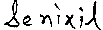
\includegraphics[width=\linewidth]{imagens/211.png}
		\caption{}
		\label{fig:211}
	\end{subfigure}
	\hfill
	\begin{subfigure}{0.15\textwidth}
		\centering
		
\includegraphics[width=\linewidth]{imagens/139.png}
		\caption{}
		\label{fig:139}
	\end{subfigure}
	\hfill
	\begin{subfigure}{0.15\textwidth}
		\centering
		
\includegraphics[width=\linewidth]{imagens/171.png}
		\caption{}
		\label{fig:171}
	\end{subfigure}
	
	\caption{Samples from PrescriptionBD}
	\label{fig:prescriptionbd}
\end{figure}
	
	


RxHandBD is a dataset developed by Md. Masudul Islam of the Bangladesh University of Business and Technology (BUBT)~\cite{islam2026rxhandbd} and made publicly available through the Zenodo and Mendeley Data repositories. The dataset was created to provide a standardized benchmark for handwritten text recognition (HTR) and optical character recognition (OCR) research applied to handwritten medical prescriptions.

The RxHandBD documentation states that the samples were obtained from physical medical prescriptions, from which individual words were segmented and subsequently annotated. However, the available documentation does not provide detailed information about the prescription acquisition process, the number of professionals who participated in the collection, or the procedures used to digitize and segment the samples. The dataset contains 5,578 word images extracted from handwritten medical prescriptions, corresponding to 1,559 distinct words. Images are provided in JPG format, while their annotations are supplied in CSV files.

\textit{RxHandBD} was selected for this study because it provides a standardized collection of words from handwritten medical prescriptions, including annotated transcriptions and an official division between training and test sets. Compared with \textit{PrescriptionBD}, this dataset presents features such as thicker letter strokes and greater expression of regional variability in medical handwriting. These differences make \textit{RxHandBD} relevant for evaluating model generalization under different handwriting patterns. From a comparative perspective, it is useful to investigate how the architectures perform on writing samples with distinct characteristics. These particularities can be observed in Figure~\ref{fig:rxhandbd}, which shows representative examples of the handwriting characteristics found in the dataset.


\begin{figure}[H]
	\centering
	
	\begin{subfigure}{0.15\textwidth}
		\centering
		
\includegraphics[width=\linewidth]{imagens/P0302.jpg}
		\caption{}
		\label{fig:p0302}
	\end{subfigure}
	\hfill
	\begin{subfigure}{0.15\textwidth}
		\centering
		
\includegraphics[width=\linewidth]{imagens/P0163.jpg}
		\caption{}
		\label{fig:p0163}
	\end{subfigure}
		\hfill
	\begin{subfigure}{0.15\textwidth}
		\centering
		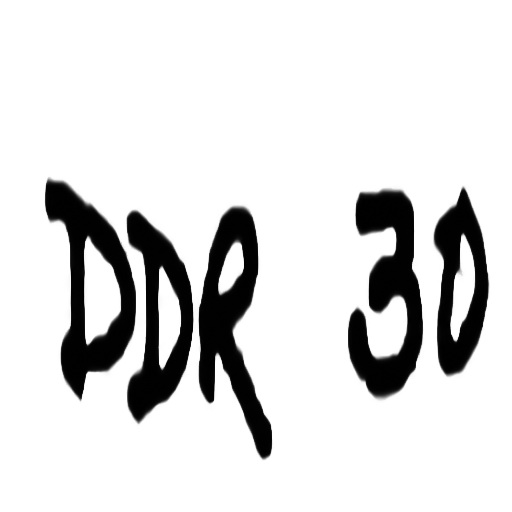
\includegraphics[width=\linewidth]{imagens/P0220.jpg}
		\caption{}
		\label{fig:p0220}
	\end{subfigure}
	
	\caption{Samples from RxHandBD}
	\label{fig:rxhandbd}
\end{figure}

As previously discussed, \textit{PrescriptionBD} contains images with non-standardized resolutions whose dimensions vary in both height and width. To ensure dataset uniformity and enable a direct comparison with \textit{RxHandBD}, a resolution of $512 \times 512$ pixels was adopted as the input standard for all evaluated architectures. This standardization is also required to convert the images into fixed-size tensors, which is fundamental for training the neural networks.

White padding was used to preserve the prescription content and avoid distortions introduced by disproportionate resizing. In this procedure, each image was placed on a white background until it reached a resolution of $512 \times 512$ pixels, preserving its original proportions and adding padding pixels only to the remaining regions. As a result, all samples acquired uniform dimensions, making them suitable for processing by the deep learning architectures and enabling a fairer methodological comparison between the datasets. Figure~\ref{fig:comp} compares an image before and after standardization: Figure~\ref{fig:stani} shows the Lenixil prescription at $103 \times 30$ pixels, whereas Figure~\ref{fig:512i} shows it after standardization to $512 \times 512$ pixels.

\begin{figure}[H]
	\centering
	
	\begin{subfigure}{0.4\textwidth}
		\centering
		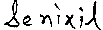
\includegraphics[width=\linewidth,height=2cm,keepaspectratio]{imagens/211.png}
		\caption{}
		\label{fig:stani}
	\end{subfigure}
	\hspace{1.5cm}
	\begin{subfigure}{0.4\textwidth}
		\centering
		
\includegraphics[width=\linewidth,height=2cm,keepaspectratio]{imagens/prescriptionbd_test_000212.png}
		\caption{}
		\label{fig:512i}
	\end{subfigure}
	
\caption{Example from \textit{PrescriptionBD} after standardization to a resolution of $512 \times 512$ pixels.}

	\label{fig:comp}
\end{figure}

Three distinct scenarios were considered in the experiments: training and evaluation exclusively on \textit{PrescriptionBD}, training and evaluation exclusively on \textit{RxHandBD}, and an additional combined scenario formed by joining the samples from both datasets. For the combined dataset, a new division into training and test sets was created according to the splits presented in Table~\ref{tab:splits}. For \textit{PrescriptionBD}, the official split provided by the authors was preserved to support experiment reproducibility and result comparability.

\begin{table}[htbp]
	\centering
	\caption{Splits used in the different experimental scenarios.}
	\label{tab:splits}
	\begin{tabular}{lrrrrl}
		\toprule
		\textbf{Scenario} & \textbf{Train} & \textbf{Val} & \textbf{Test} & \textbf{Total} & \textbf{Method} \\
		\midrule
		RxHandBD       & 3905 & 837  & 836  & 5578  & 70/15/15 by sample, seed 757 \\
		PrescriptionBD & 3120 & 780  & 780  & 4680  & Official split preserved \\
		Combined       & 7025 & 1617 & 1616 & 10258 & Union of the corresponding splits \\
		\bottomrule
	\end{tabular}
\end{table}


Because of the limited number of samples available for training, data augmentation was used to increase data variability and reduce the risk of model overfitting. The transformations were applied randomly during training, generating different variations of the same image in each epoch.

Three data augmentation techniques were used. The first was \textit{RandomAffine}, which applies random rotations and translations to the images with a probability of $90\%$. The second was \textit{ColorJitter}, which randomly changes image brightness and contrast, with variations of $0.25$ for brightness and $0.35$ for contrast, and was applied with a probability of $60\%$. Finally, \textit{GaussianBlur} was used with a kernel size of 3 and $\sigma$ values ranging from $0.1$ to $0.8$, with an application probability of $30\%$. Figure~\ref{fig:data-augmentation-examples} shows the result of applying this augmentation methodology to a sample from \textit{RxHandBD}.

\begin{figure}[H]
	\centering
	
	\begin{subfigure}[b]{0.25\textwidth}
		\centering
		
\includegraphics[width=\linewidth]{
			imagens/rxhandbd_000001_original.png
		}
		\caption{Original image}
		\label{fig:augmentation-original}
	\end{subfigure}
		\vspace{0.8cm}
	\begin{subfigure}[b]{0.25\textwidth}
		\centering
		
\includegraphics[width=\linewidth]{
			imagens/rxhandbd_000001_random_affine.png
		}
		\caption{Random Affine}
		\label{fig:augmentation-affine}
	\end{subfigure}
	
	\vspace{0.4cm}
	
	\begin{subfigure}[b]{0.25\textwidth}
		\centering
		
\includegraphics[width=\linewidth]{
			imagens/rxhandbd_000001_colorjitter.png
		}
		\caption{ColorJitter}
		\label{fig:augmentation-colorjitter}
	\end{subfigure}
	\vspace{0.8cm}
	\begin{subfigure}[b]{0.25\textwidth}
		\centering
		
\includegraphics[width=\linewidth]{
			imagens/rxhandbd_000001_blur.png
		}
		\caption{Gaussian blur}
		\label{fig:augmentation-blur}
	\end{subfigure}
	
	\caption{Example of data augmentation transformations applied to a sample from the RxHandBD training set.}
	\label{fig:data-augmentation-examples}
\end{figure}

These transformations supported more consistent training with a lower occurrence of overfitting.


\subsection{Computational Models}
\label{sec:models}

Four architectures were used in this study: a CNN baseline, a CNN-BiLSTM, TrOCR, and PARSeq.

\subsubsection{CNN Baseline}



Convolutional Neural Networks (CNNs) are inspired by principles observed in the biological visual system, particularly the studies of the visual cortex conducted by Hubel and Wiesel~\cite{hubel1962receptive}. Although they do not faithfully reproduce how the human brain operates, these architectures were conceived from the observation that the visual system can recognize complex patterns through hierarchical combinations of simple visual features.

In the experiments conducted by Hubel and Wiesel, neurons in the visual cortex were found to respond selectively to specific stimuli such as edges, orientations, and contrasts. Visual information processing was also observed to occur hierarchically, with higher-level neurons integrating information extracted by simpler neurons to represent increasingly complex structures~\cite{hubel1962receptive}.

Inspired by these principles, CNNs introduce local receptive fields through convolutional layers, in which filters automatically learn patterns present in the images. As multiple convolutional layers are stacked, hierarchical feature representations can be constructed, beginning with basic elements such as edges and textures and progressing toward more complex patterns such as shapes and objects. This organization has made CNNs one of the main architectures used in computer vision and pattern recognition tasks.


The conceptual foundations of modern CNN models can be traced to Fukushima's work, presented in \textit{Neocognitron: A Self-Organizing Neural Network Model for a Mechanism of Pattern Recognition Unaffected by Shift in Position}~\cite{fukushima1980neocognitron}. That study proposed a hierarchical architecture inspired by the visual cortex, with layers responsible for progressive feature extraction and invariance to small translations in the input patterns. Although the Neocognitron did not use \textit{backpropagation} training, its architectural principles helped establish the foundation for modern CNNs.

LeCun et al.~\cite{lecun1998gradient} later consolidated this paradigm by presenting a convolutional architecture trained with \textit{backpropagation} for optical character recognition (OCR), demonstrating that automatically learned convolutional filters could achieve high performance in pattern recognition tasks. This work established a practical basis for the widespread adoption of CNNs in computer vision problems.

In this study, the CNN was used as a reference model (\textit{baseline}), representing the starting point for comparison among the evaluated architectures. It establishes an initial performance level for traditional convolutional models in handwritten medical prescription recognition and provides a basis for analyzing the gains obtained with more sophisticated architectures.

However, the problem addressed in this work differs from a conventional image classification task. The objective is to recognize complete words in prescriptions, which characterizes a sequence recognition problem. A conventional CNN produces only one classification for each input image, preventing it from directly predicting all characters that form a word in a single inference.

To address this limitation, the CNN \textit{baseline} was formulated as a word classifier. In this approach, each word in the training set is treated as a distinct class. The network output therefore corresponds to a probability distribution over all known classes, and the word with the highest probability is selected as the prediction. The model does not perform sequential character recognition; instead, it directly estimates which previously learned word corresponds to the input image.

As an extension of the CNN \textit{baseline}, an architecture incorporating a \textit{Bidirectional Long Short-Term Memory} (BiLSTM) layer was developed. This modification allows the model to move beyond the classification of previously known words and recognize the character sequence in the image, making it more suitable for handwritten text recognition tasks.

\newpage
\subsubsection{CNN BiLSTM}

To improve recognition accuracy, a \textit{Bidirectional Long Short-Term Memory} (BiLSTM) module was incorporated into the CNN baseline. This architecture is a recurrent neural network capable of modeling long-range sequential dependencies by processing a sequence in both the forward and backward directions~\cite{shi2016crnn}. The model can therefore consider not only the current element but also the context supplied by preceding and subsequent characters.

The inclusion of the BiLSTM is motivated by the inherent sequential structure of handwritten words. In a language, some characters are more likely to occur together, including common alternations between consonants and vowels and the spelling patterns associated with each word. By exploring these contextual dependencies, the BiLSTM complements the visual features extracted by the CNN, allowing the classification process to consider both character appearance and the sequential relationships among characters. The CNN-BiLSTM architecture was therefore evaluated for its ability to improve handwritten medical prescription recognition relative to the CNN baseline.

After incorporating the BiLSTM, the architecture produced temporal outputs and was trained with CTC over a character vocabulary. During greedy decoding, consecutive repetitions and the blank symbol are removed to reconstruct the predicted word. Unlike the CNN \textit{baseline}, CNN-BiLSTM is therefore not restricted to a closed set of word classes and can form sequences that were not observed during training, provided that their characters belong to the learned vocabulary.

To broaden the comparison with sequence architectures initialized through large-scale pre-training, Transformer-based models were subsequently evaluated. These models also perform recognition at the character-sequence level and can recognize words that were not present in the training set.


\subsubsection{TrOCR}

TrOCR (Transformer-based Optical Character Recognition) is an optical character recognition model proposed by Li et al.~\cite{li2023trocr} that uses an encoder-decoder architecture based entirely on Transformers. The model employs a visual Transformer to extract representations from the input image and a textual Transformer to generate the corresponding sequence of characters or tokens, eliminating the need for traditional CNN-, RNN-, and CTC-based architectures. TrOCR can also be pre-trained on large synthetic datasets and subsequently fine-tuned with labeled data, with applications to printed, handwritten, and scene text.

\subsubsection{PARSeq}

PARSeq (Permuted Autoregressive Sequence) is a Transformer-based model developed for text recognition in images, particularly in the context of Scene Text Recognition~\cite{bautista2022parseq}. Unlike conventional autoregressive models, which generate characters only from left to right, PARSeq uses Permutation Language Modeling, allowing the model to learn different prediction orders and explore bidirectional context during recognition. This approach combines autoregressive inference, non-autoregressive inference, and iterative refinement within a single architecture, providing a balance among accuracy, parameter count, and computational cost.
\subsection{Baselines and Metrics}
\label{sec:baselines}

An experiment matrix was initially defined to establish the training and test sets used for each model. This standardization enabled systematic evaluation with consistent metrics, making it possible to analyze the performance of each architecture and understand the factors that influenced the results. The results from all experiments were then compared.

To support a fair comparison among the architectures, specific comparison matrices were defined for each group of experiments. These matrices consider the conceptual differences among the models and their training particularities, avoiding inappropriate comparisons between distinct approaches. This procedure made it possible to evaluate the generalization capability and performance of each architecture under different scenarios and quantities of training data.

All experiments are presented in Table~\ref{tab:matriz-experimentos}.
\begin{table}[H]
	\centering
	\caption{Experiment matrix by architecture and dataset.}
	\label{tab:matriz-experimentos}
	\begin{tabular}{cllrrr}
		\toprule
		\textbf{Exp.} &
		\textbf{Architecture} &
		\textbf{Dataset} &
		\textbf{Train} &
		\textbf{Validation} &
		\textbf{Test} \\
		\midrule
		
		E1 & CNN baseline & PrescriptionBD & 3120 & 780  & 780  \\
		E1 & CNN baseline & RxHandBD       & 3905 & 837  & 836  \\
		E1 & CNN baseline & Combined       & 7025 & 1617 & 1616 \\
		\midrule
		
		E2 & CNN-BiLSTM   & PrescriptionBD & 3120 & 780  & 780  \\
		E2 & CNN-BiLSTM   & RxHandBD       & 3905 & 837  & 836  \\
		E2 & CNN-BiLSTM   & Combined       & 7025 & 1617 & 1616 \\
		\midrule
		
		E3 & TrOCR        & PrescriptionBD & 3120 & 780  & 780  \\
		E3 & TrOCR        & RxHandBD       & 3905 & 837  & 836  \\
		E3 & TrOCR        & Combined       & 7025 & 1617 & 1616 \\
		\midrule
		
		E4 & PARSeq       & PrescriptionBD & 3120 & 780  & 780  \\
		E4 & PARSeq       & RxHandBD       & 3905 & 837  & 836  \\
		E4 & PARSeq       & Combined       & 7025 & 1617 & 1616 \\
		\bottomrule
	\end{tabular}
\end{table}

Throughout training, performance metrics were collected at each epoch to characterize the progression of model learning. The loss values on the training and validation sets and the accuracy achieved on both sets were recorded.

The models were evaluated using metrics that capture different aspects of text recognition performance. Accuracy measured whether the model correctly recognized the complete character sequence in an image. Character Error Rate (CER) quantified character-level errors through the number of insertions, deletions, and substitutions required to transform the prediction into the reference text. Word Error Rate (WER) complemented this analysis by measuring word-level errors as the number of incorrectly recognized words relative to the expected text.

\subsection{Implementation Details}
\label{sec:implementation}

The experiments were implemented in Python using the package developed for this
project, named \texttt{med-ocr-research}. The execution environment uses Python
3.10 or later, with PyTorch as the main deep learning framework. All training
runs were performed with CUDA acceleration on an NVIDIA GeForce RTX 3050 GPU
with 6 GB of memory. The complete computational environment configuration is
shown in Table~\ref{tab:hardware}.

The main dependencies used during development are presented in
Table~\ref{tab:software}. The listed values represent the minimum versions used
in the experimental environment. For TrOCR, the pre-trained model files record
the use of Transformers version 5.12.1.

\begin{table}[htbp]
	\centering
	\caption{Software dependencies used in the experimental environment.}
	\label{tab:software}
	\begin{tabular}{llll}
		\toprule
		\textbf{Library} & \textbf{Version} &
		\textbf{Library} & \textbf{Version} \\
		\midrule
		Python            & $\geq 3.10$   & PyTorch          & $\geq 2.2$  \\
		Torchvision       & $\geq 0.17$   & Transformers     & 5.12.1       \\
		NumPy             & $\geq 1.24$   & Pandas           & $\geq 2.0$  \\
		Pillow            & $\geq 10.0$   & Timm             & $\geq 1.0$  \\
		PyTorch Lightning & $\geq 2.2$    & Accelerate       & $\geq 0.30$ \\
		Albumentations    & $\geq 1.4$    & SentencePiece    & $\geq 0.2.1$ \\
		NLTK              & $\geq 3.8$    & Tqdm             & $\geq 4.66$ \\
		PyYAML            & $\geq 6.0$    & Protobuf         & $\geq 4.25$ \\
		\bottomrule
	\end{tabular}
\end{table}

The random seed 42 was used throughout all experiments to support result
reproducibility. This seed was applied to the generators from the
\texttt{random}, NumPy, and PyTorch libraries, including CUDA initialization
through \texttt{torch.cuda.manual\_seed\_all}. The official PrescriptionBD split
was preserved when organizing the datasets. RxHandBD was divided into 70\% for
training, 15\% for validation, and 15\% for testing using the derived seed 757.
The combined dataset was obtained by joining the corresponding subsets from the
two datasets.

The CNN baseline and CNN-BiLSTM were implemented in this project. TrOCR used the
pre-trained \nolinkurl{microsoft/trocr-small-handwritten} checkpoint. PARSeq used
the implementation available in the \nolinkurl{baudm/parseq} repository, fixed at
the following commit:
\begin{center}
	\texttt{1902db043c029a7e03a3818c616c06600af574be}
\end{center}
All developed source code, experimental configurations, and evaluation scripts
are available in the project repository:

\begin{center}
	\url{https://github.com/SamuelFerrc/Medical-Handwriting-Ocr}
\end{center}


\section{Results and Discussion}
\label{sec:results}

This section presents the results from twelve evaluations: four model families,
each evaluated on PrescriptionBD, RxHandBD, and the combined scenario. The
results are organized to support discussion at three levels: (i) aggregate
comparison among models, (ii) dataset effects, and (iii) diagnostic analysis of
each evaluation. The metrics were recalculated directly from the evaluated
prediction files. Detailed tables remain available in the artifact folder for
consultation but are not included in the main article in order to keep the
results section concise.

\subsection{Overall comparison}
\label{sec:results-overall}

The aggregate comparison by model and scenario is presented in
Figures~\ref{fig:comparison-accuracy}, \ref{fig:comparison-cer}, and
\ref{fig:comparison-wer}, which show exact-match accuracy, CER, and WER,
respectively, for all twelve evaluations.

In addition to the graphs, Table~\ref{tab:evaluation-summary-all} presents the
aggregate metrics for each model and scenario in a compact format.

% Metrics recalculated from evaluated_predictions.csv; CER/WER are aggregated as total errors divided by total reference units.
\begin{table}[htbp]
\centering
\caption{Evaluation summary by model and scenario}
\label{tab:evaluation-summary-all}
\scriptsize
\setlength{\tabcolsep}{2pt}
\resizebox{\textwidth}{!}{%
\begin{tabular}{llrrrrrr}
\toprule
\textbf{Model} & \textbf{Scenario} & \textbf{N} & \textbf{Correct} & \textbf{Accuracy} & \textbf{CER} & \textbf{WER} & \textbf{Mean confidence} \\
\midrule
CNN & PrescriptionBD & 780 & 322 & 0.4128 & 0.5328 & 0.5911 & 0.2728 \\
CNN & RxHandBD & 836 & 262 & 0.3134 & 0.5866 & 0.7313 & 0.2831 \\
CNN & Combined & 1616 & 463 & 0.2865 & 0.6467 & 0.7412 & 0.2458 \\
CNN-BiLSTM & PrescriptionBD & 780 & 527 & 0.6756 & 0.1868 & 0.3278 & 0.9822 \\
CNN-BiLSTM & RxHandBD & 836 & 436 & 0.5215 & 0.1811 & 0.4984 & 0.9767 \\
CNN-BiLSTM & Combined & 1616 & 927 & 0.5736 & 0.2064 & 0.4370 & 0.9823 \\
TrOCR & PrescriptionBD & 780 & 693 & 0.8885 & 0.0864 & 0.1127 & 0.9886 \\
TrOCR & RxHandBD & 836 & 612 & 0.7321 & 0.1122 & 0.2824 & 0.9745 \\
TrOCR & Combined & 1616 & 1307 & 0.8088 & 0.1024 & 0.2018 & 0.9826 \\
PARSeq & PrescriptionBD & 780 & 703 & 0.9013 & 0.0680 & 0.1000 & 0.9649 \\
PARSeq & RxHandBD & 836 & 579 & 0.6926 & 0.1067 & 0.3130 & 0.8880 \\
PARSeq & Combined & 1616 & 1270 & 0.7859 & 0.0943 & 0.2214 & 0.9344 \\
\bottomrule
\end{tabular}%
}
\end{table}


\begin{figure}[H]
  \centering
  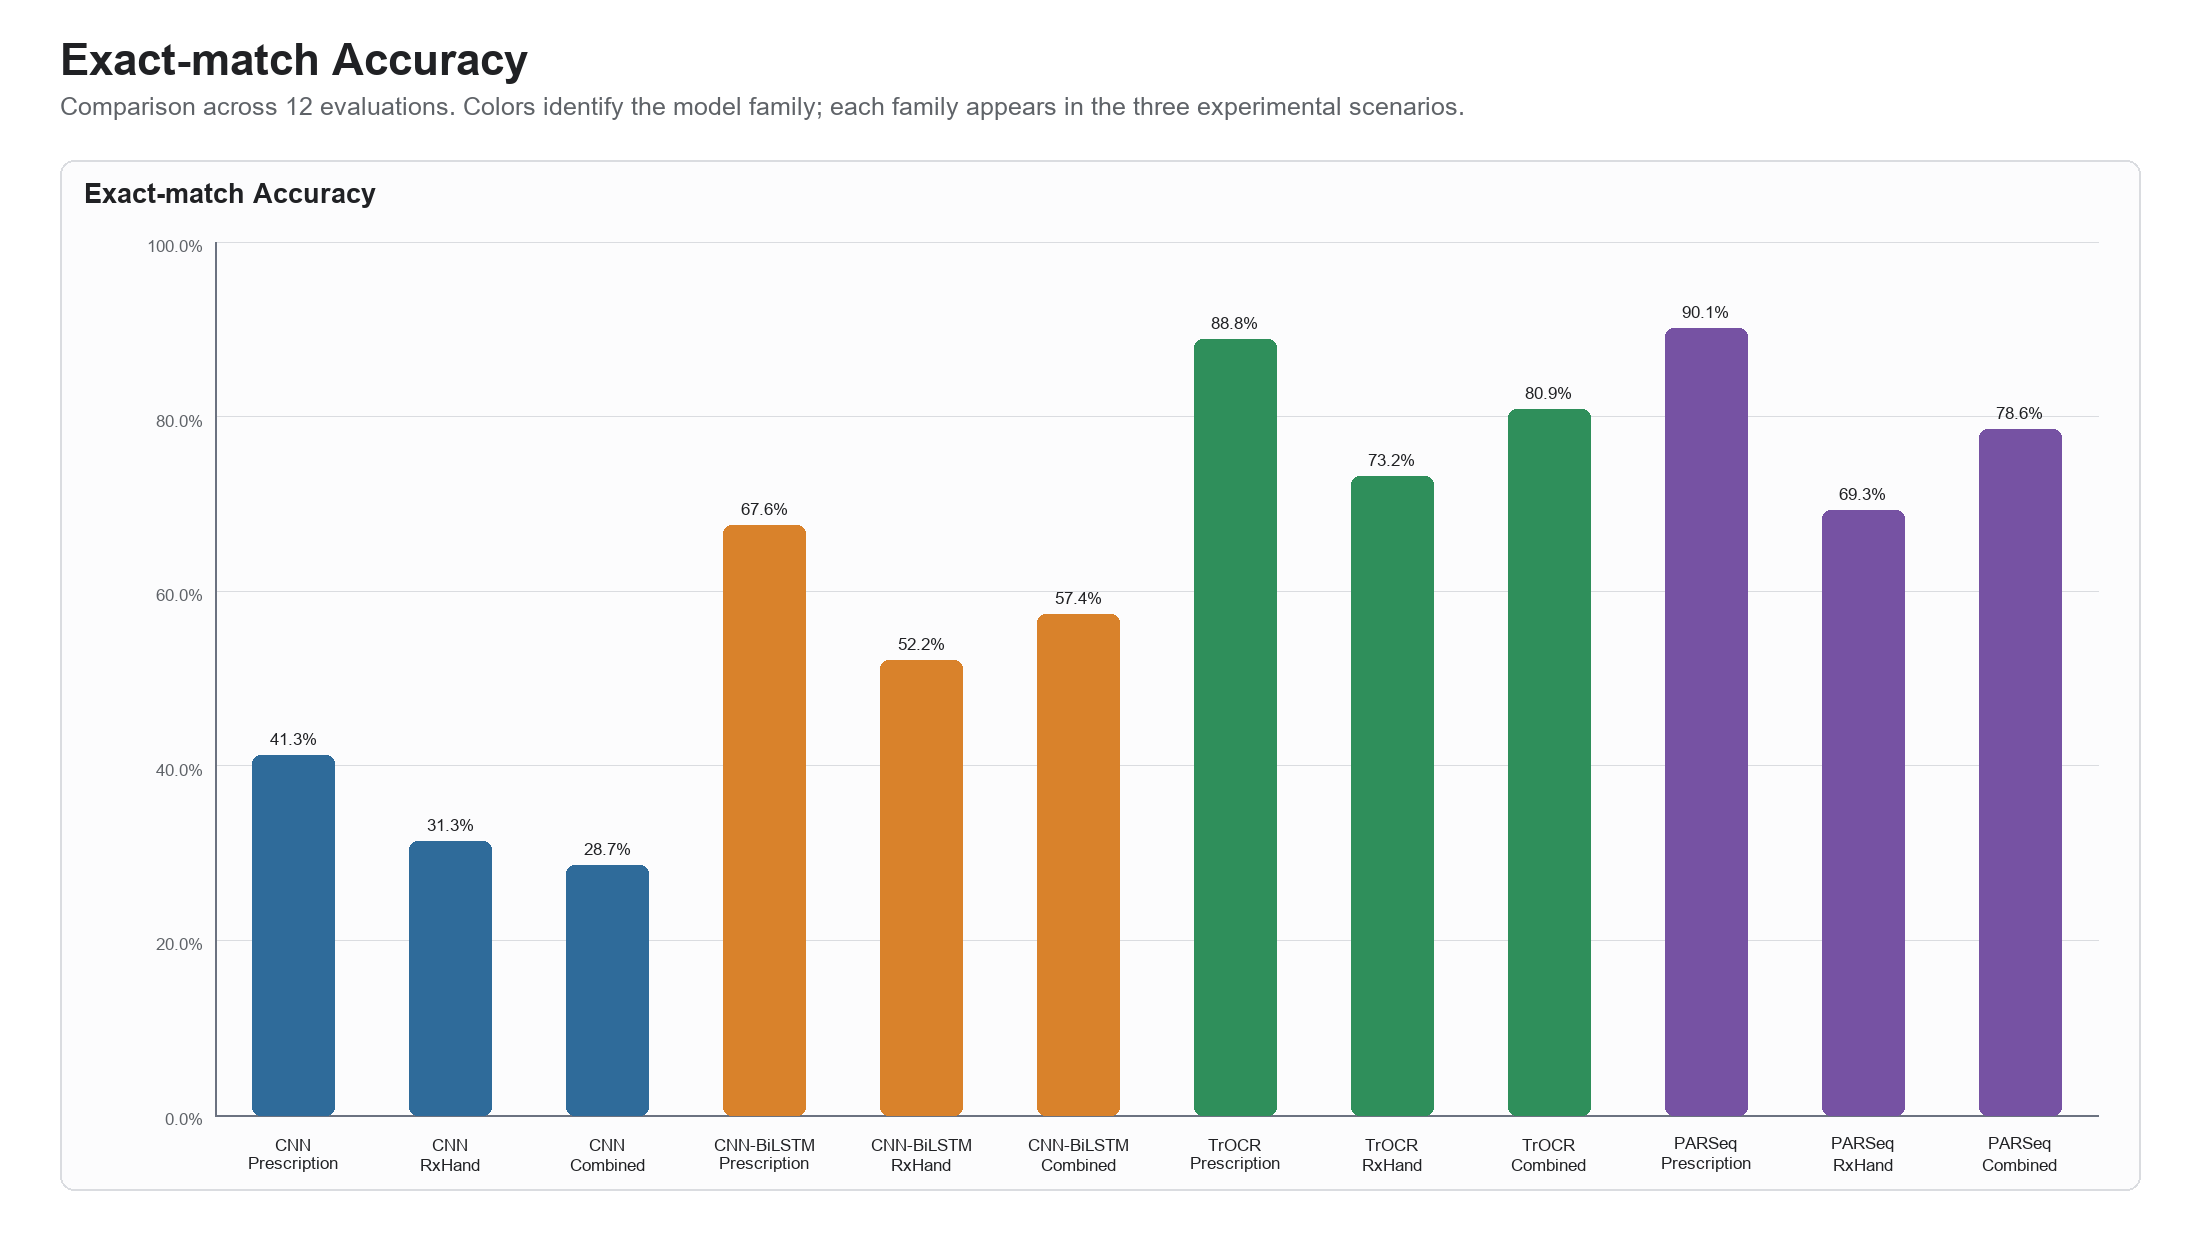
\includegraphics[width=0.94\linewidth]{imagens/evaluation_graficos_tabelas/comparison_all_evaluations_accuracy.png}
  \caption{Exact-match accuracy across all twelve evaluations.}
  \label{fig:comparison-accuracy}
\end{figure}

\begin{figure}[H]
  \centering
  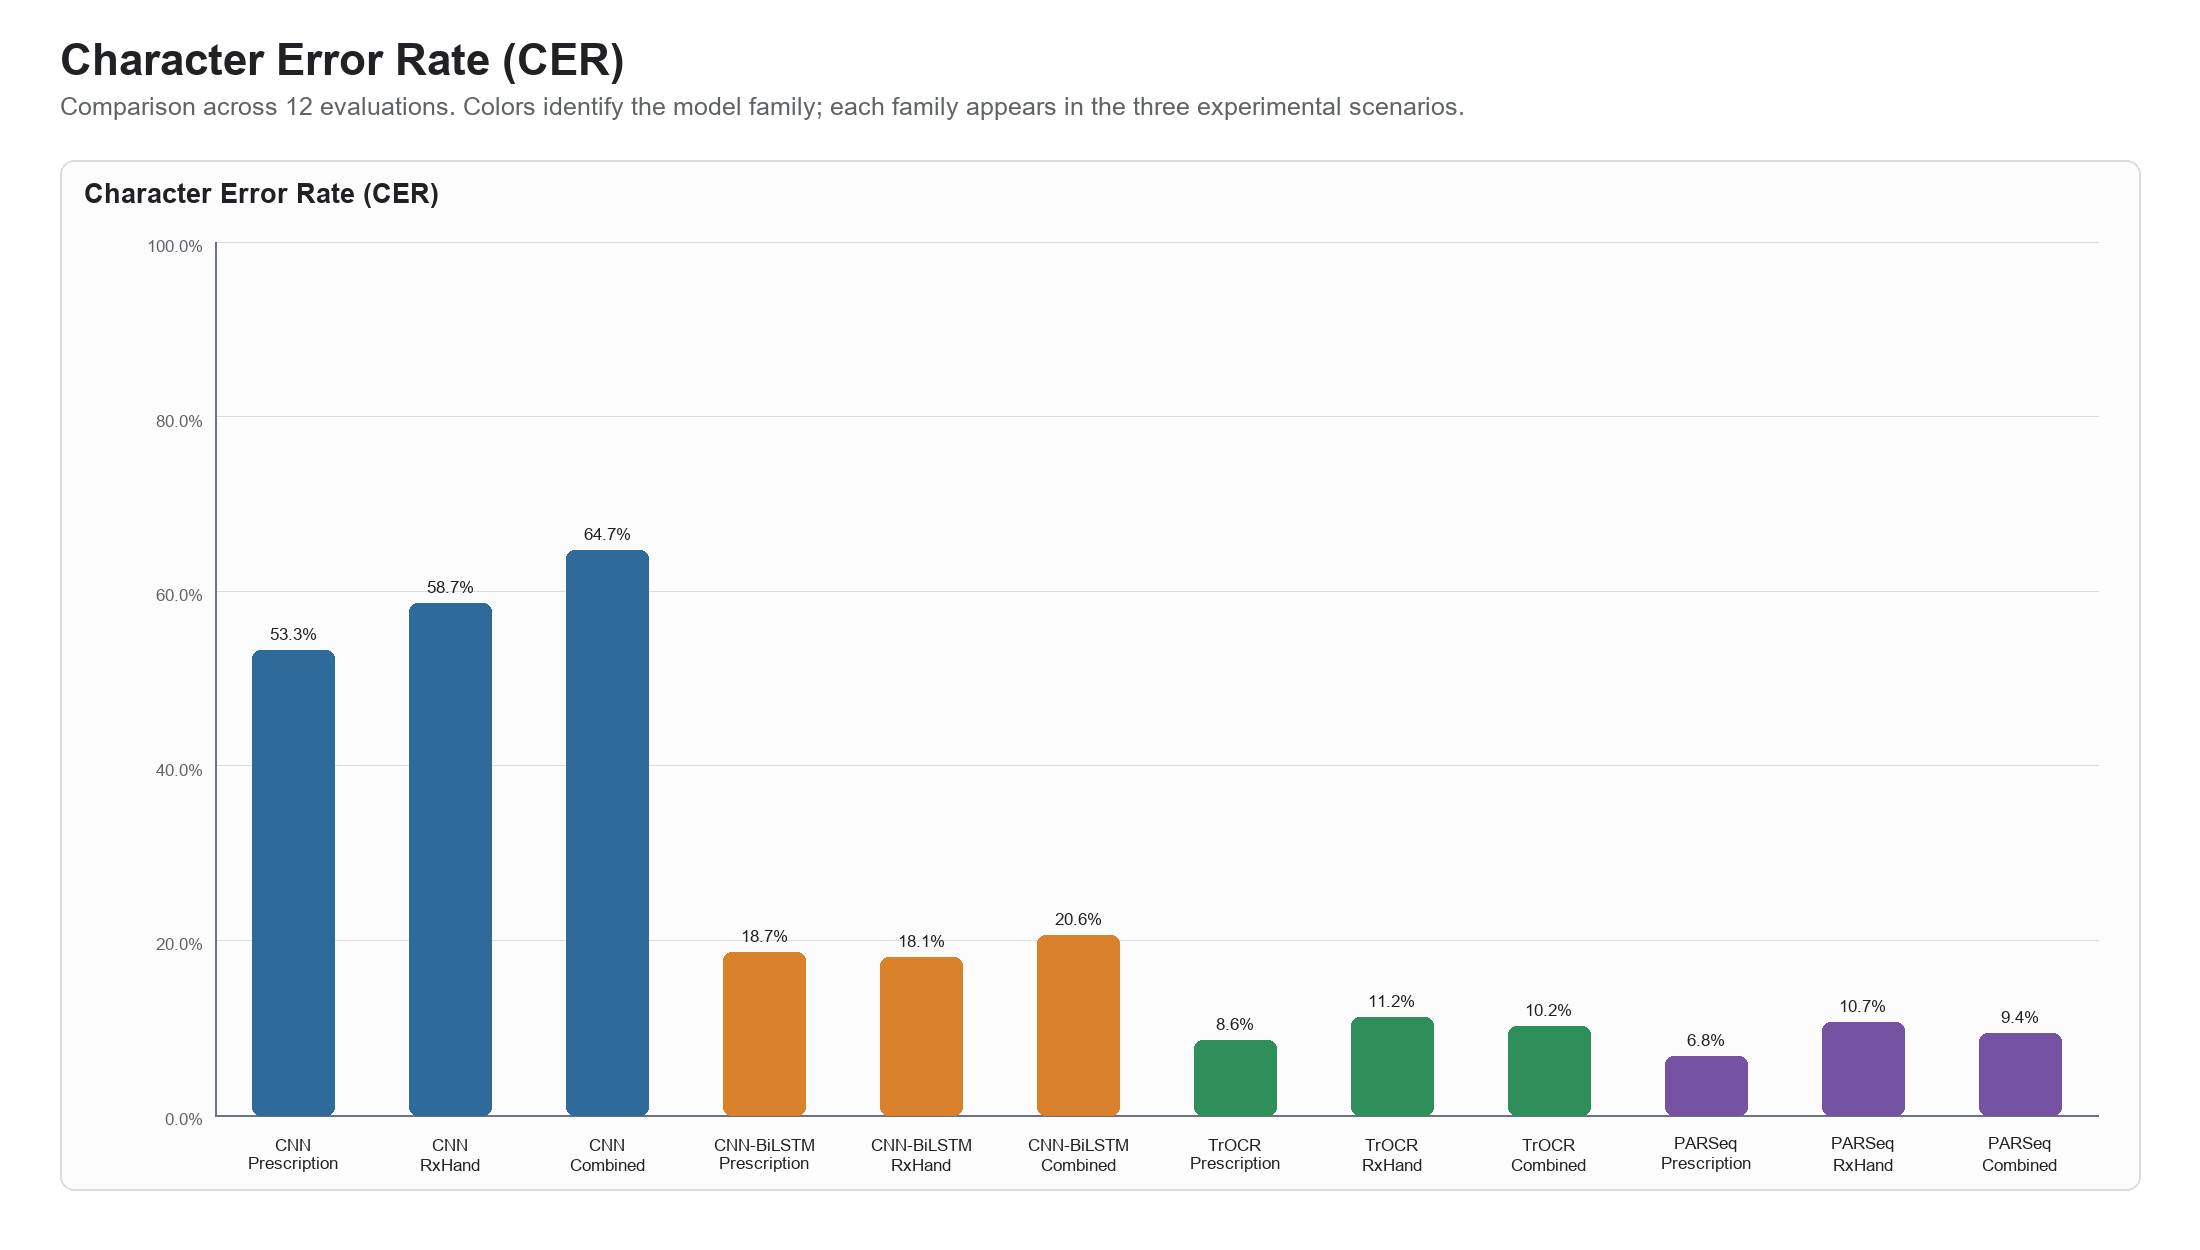
\includegraphics[width=0.94\linewidth]{imagens/evaluation_graficos_tabelas/comparison_all_evaluations_cer.png}
  \caption{Character Error Rate (CER) across all twelve evaluations.}
  \label{fig:comparison-cer}
\end{figure}

\begin{figure}[H]
  \centering
  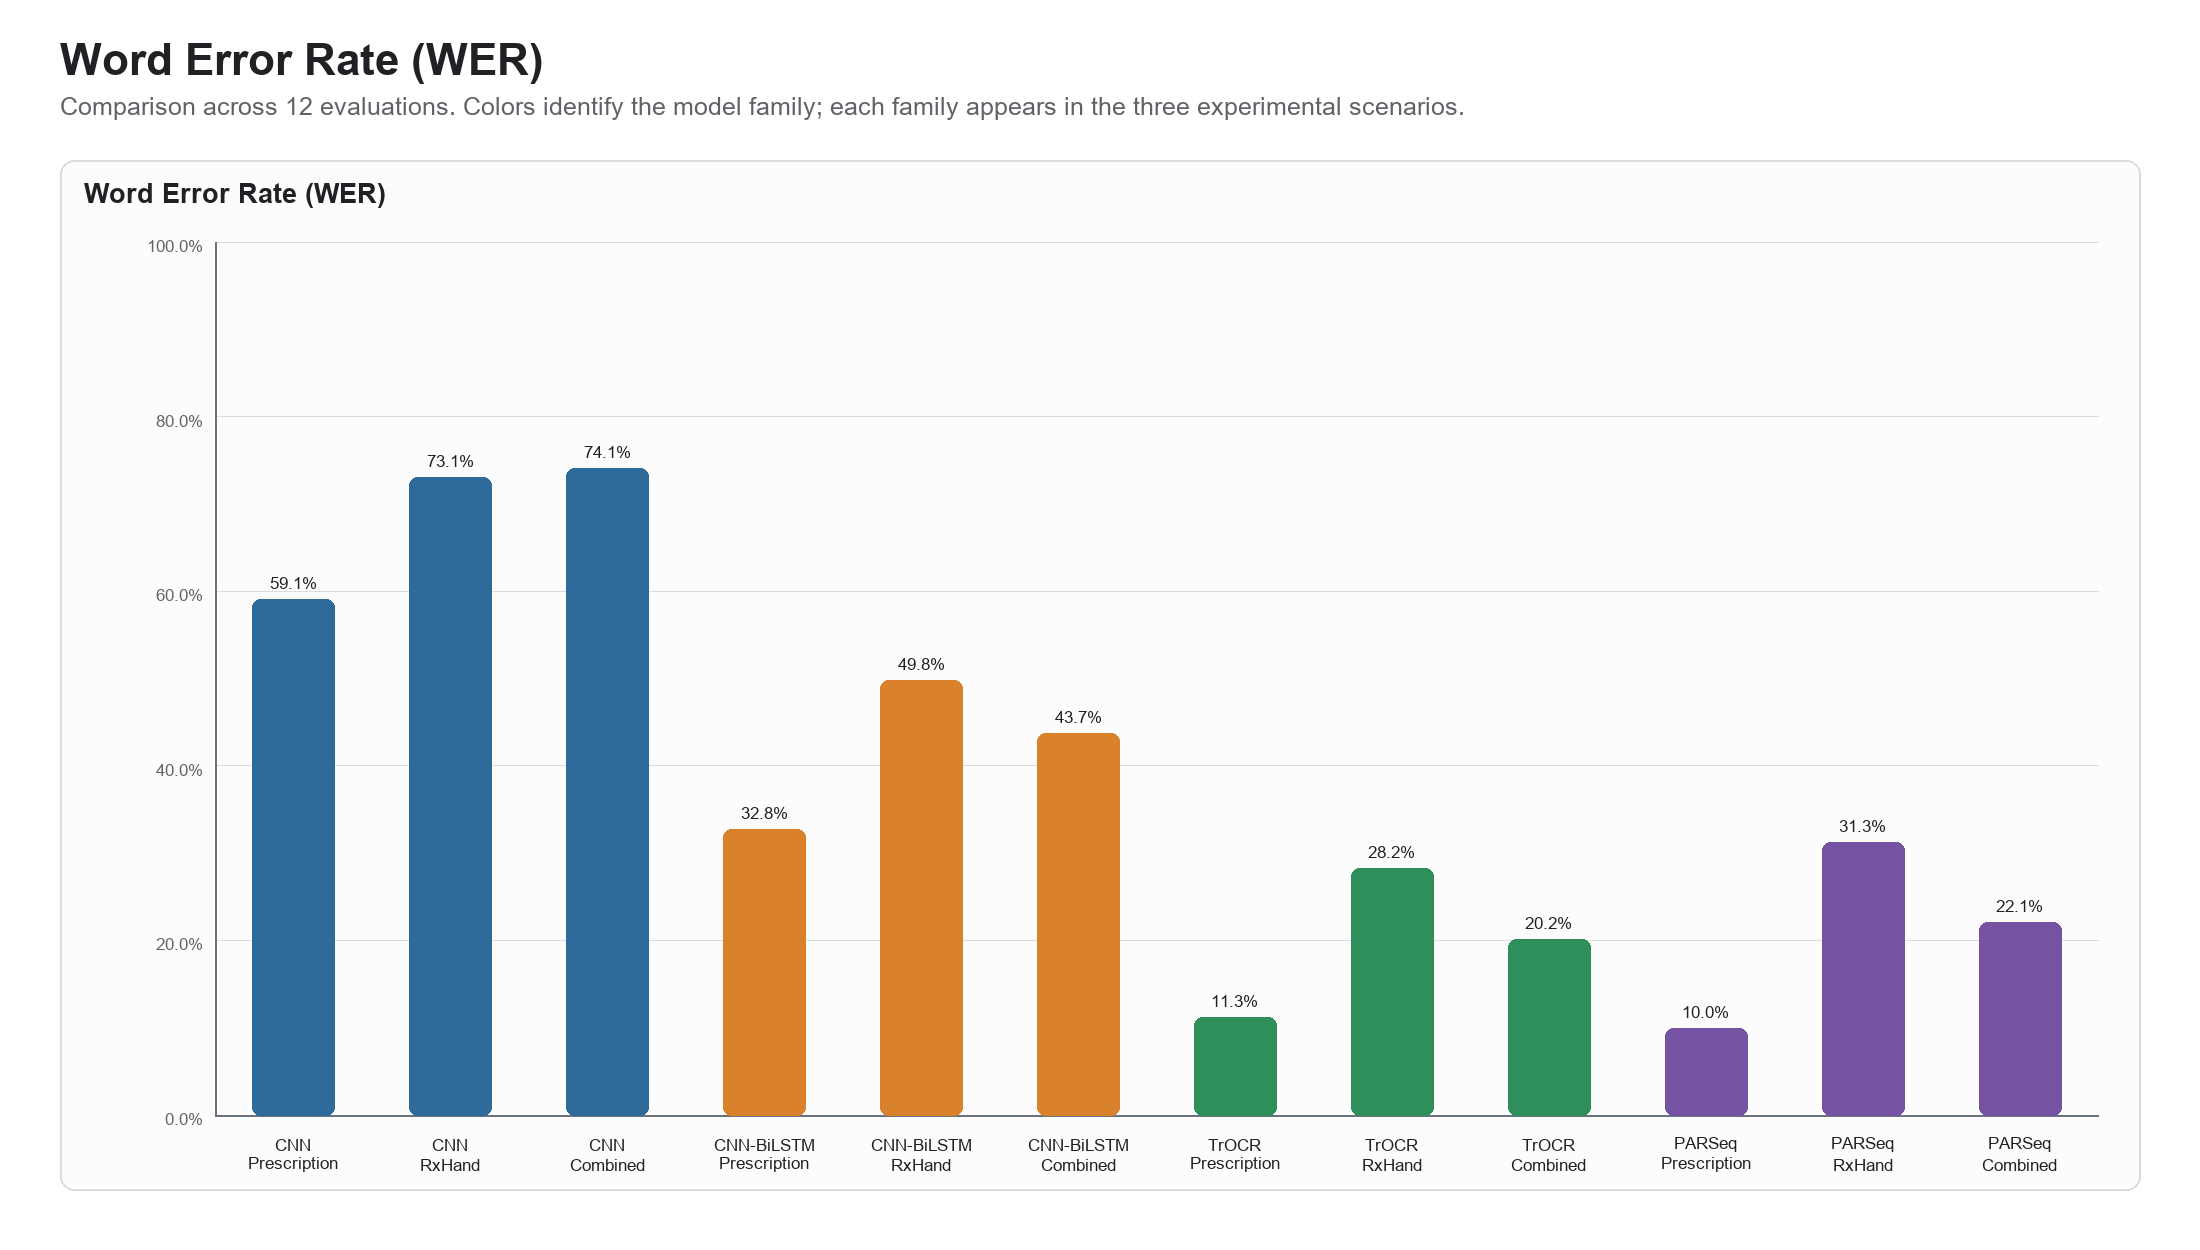
\includegraphics[width=0.94\linewidth]{imagens/evaluation_graficos_tabelas/comparison_all_evaluations_wer.png}
  \caption{Word Error Rate (WER) across all twelve evaluations.}
  \label{fig:comparison-wer}
\end{figure}

The results in Figure~\ref{fig:comparison-accuracy} show that all models achieved their best performance on PrescriptionBD. This pattern was not observed on RxHandBD, where most models performed worse, except for the CNN baseline, which produced relatively more consistent results.

This difference may be associated primarily with the visual characteristics of each dataset. As illustrated in Figure~\ref{fig:rxhandbd}, RxHandBD images contain thicker, more blurred, and less clearly defined strokes, making it more difficult for both CNNs and Transformer-based models to extract discriminative features. In contrast, Figure~\ref{fig:prescriptionbd} shows that PrescriptionBD contains characters with thinner, more continuous, and better-defined strokes, which may facilitate pattern identification and the learning of more robust representations by the neural networks. The observed visual-quality differences between the datasets are therefore consistent with the differences in model performance during training and inference.

The experiments on the combined dataset produced intermediate performance relative to the two original datasets. This behavior was expected because the combined set includes both the favorable characteristics of PrescriptionBD and the challenges present in RxHandBD. The models were exposed to higher-quality examples as well as samples with greater visual complexity, resulting in average performance between the two original scenarios.

One notable result was that CNN-BiLSTM achieved a lower CER on RxHandBD than on PrescriptionBD, as shown in Figure~\ref{fig:comparison-cer}. This result indicates that, although RxHandBD was more challenging for most of the evaluated models, CNN-BiLSTM recognized individual characters more accurately in this specific scenario.

Across all evaluated models and datasets, WER behaved consistently with overall accuracy, as illustrated in Figure~\ref{fig:comparison-wer}. In general, models with higher accuracy also had lower WER values, showing the inverse relationship between these metrics and supporting the consistency of the experimental results.

\subsection{Dataset-specific comparison}
\label{sec:results-dataset}

To separate the effect of the combined scenario from the effect of the
architecture, Figure~\ref{fig:comparison-combined-dataset} presents the
comparison of accuracy, CER, and WER by dataset.

\begin{figure}[H]
  \centering
  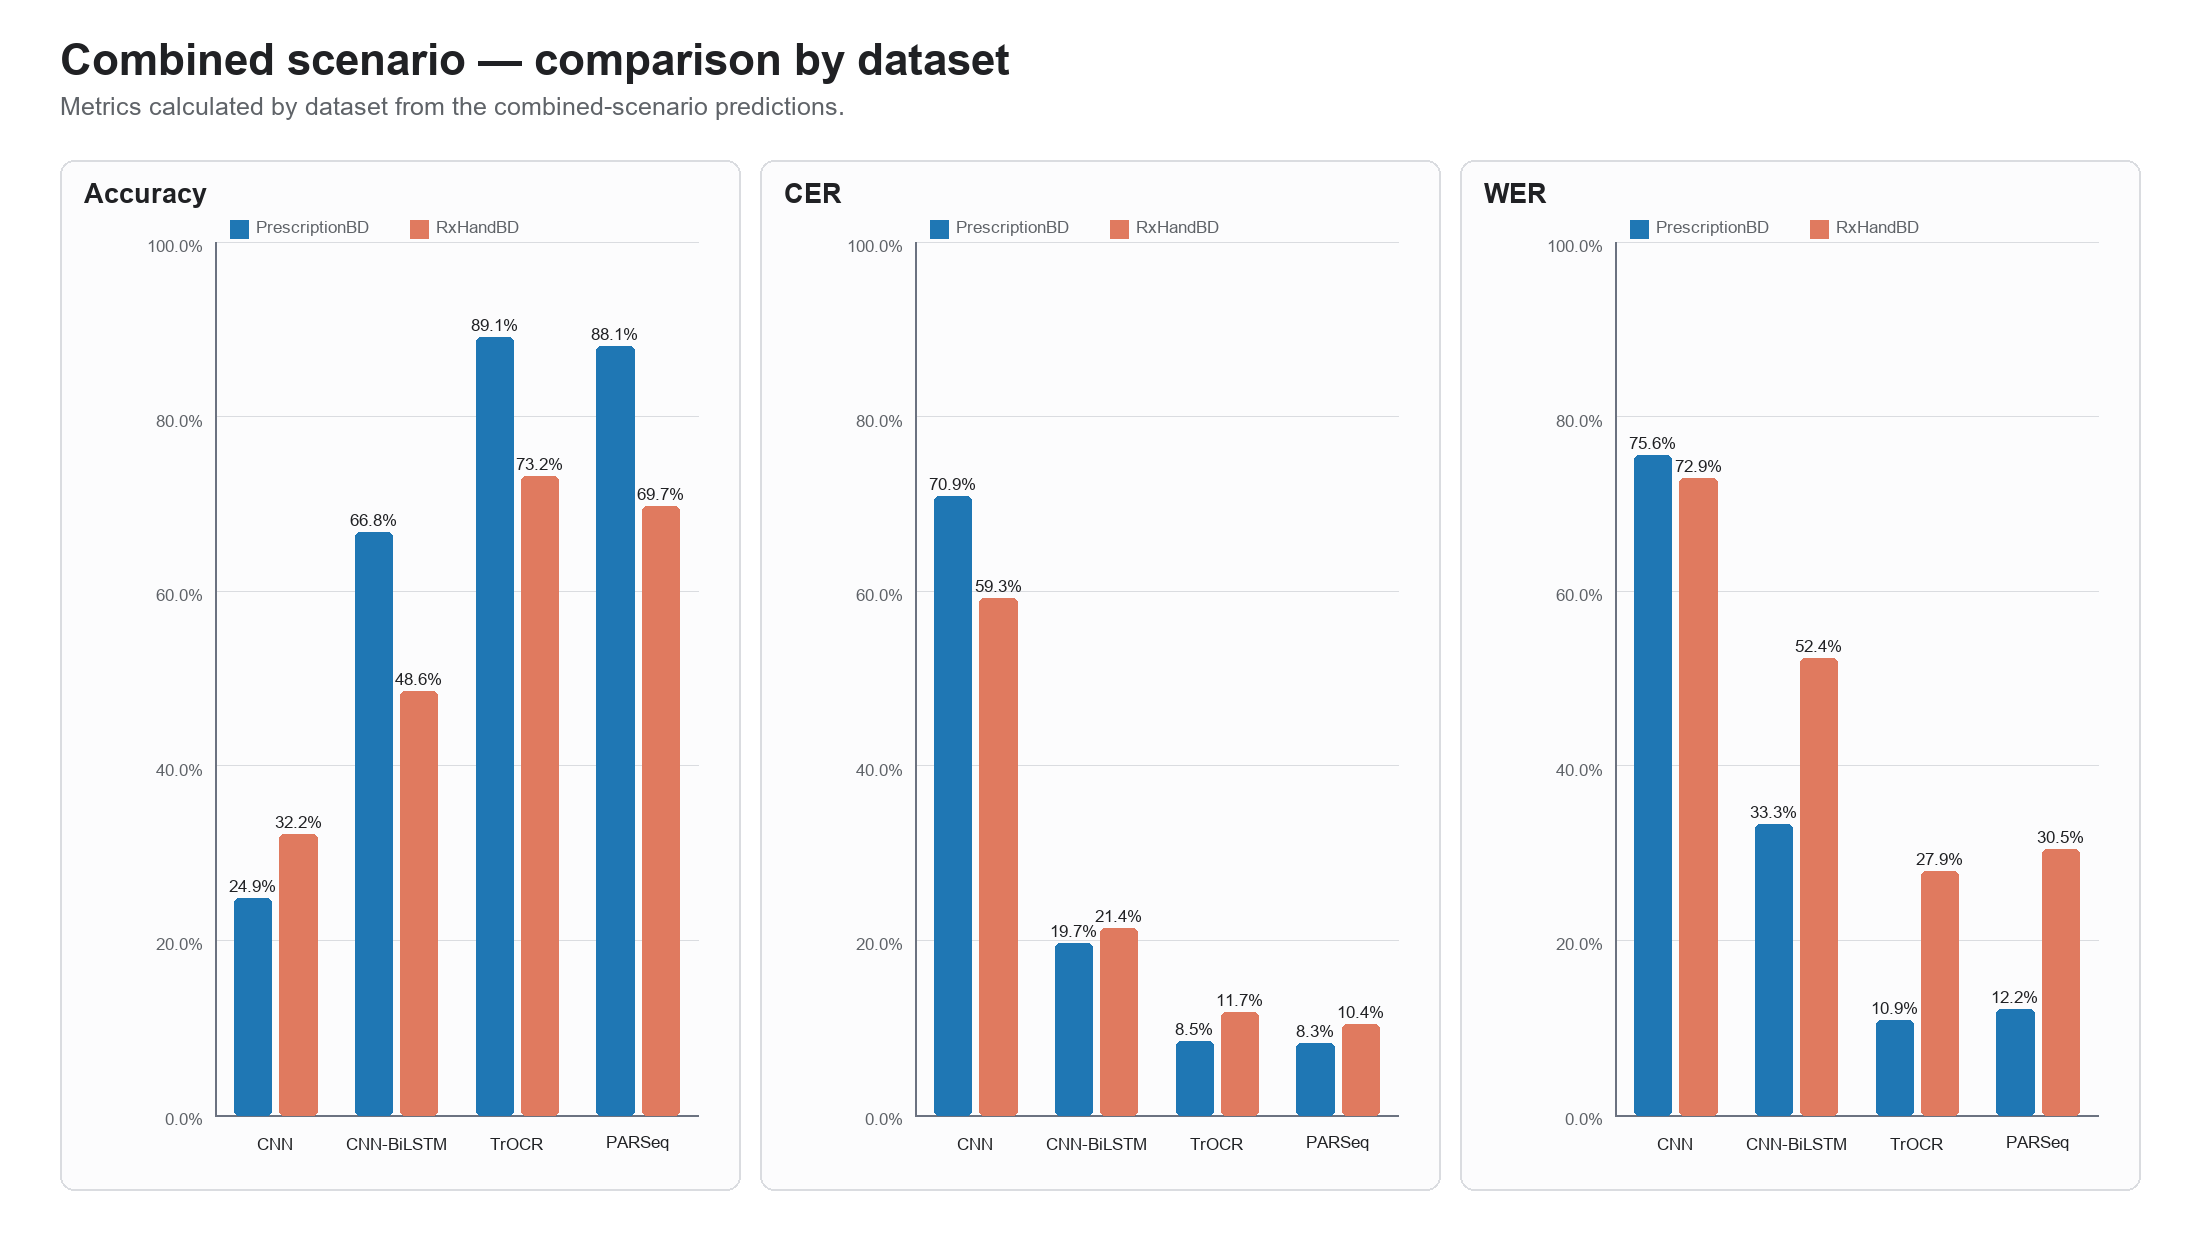
\includegraphics[width=0.94\linewidth]{imagens/evaluation_graficos_tabelas/comparison_combined_by_dataset.png}
  \caption{Comparison of the combined scenario by dataset.}
  \label{fig:comparison-combined-dataset}
\end{figure}

For each neural network model, the difference between the results represented by the blue and orange bars was calculated for overall accuracy. The CNN baseline was the only model for which the orange bar exceeded the blue bar, with a difference of 7.3 percentage points. For the remaining models, the blue bar showed better performance, with differences of 18.2 percentage points for CNN-BiLSTM, 15.9 percentage points for TrOCR, and 18.4 percentage points for PARSeq.

\subsection{Per-evaluation diagnostic views}
\label{sec:results-diagnostics}

The figures in this subsection complement the aggregate metrics. Each evaluated
prediction panel includes the error distribution, the relationship between
performance and reference length, and accuracy by confidence range. The
per-label panel shows the distribution of performance across words, highlighting
the most frequent labels and those with the lowest accuracy. These panels are
descriptive and should be used to investigate error patterns rather than as
substitutes for the aggregate metrics.

\subsubsection{CNN baseline}

\begin{figure}[H]
  \centering
  \begin{subfigure}{0.49\linewidth}
    \centering
    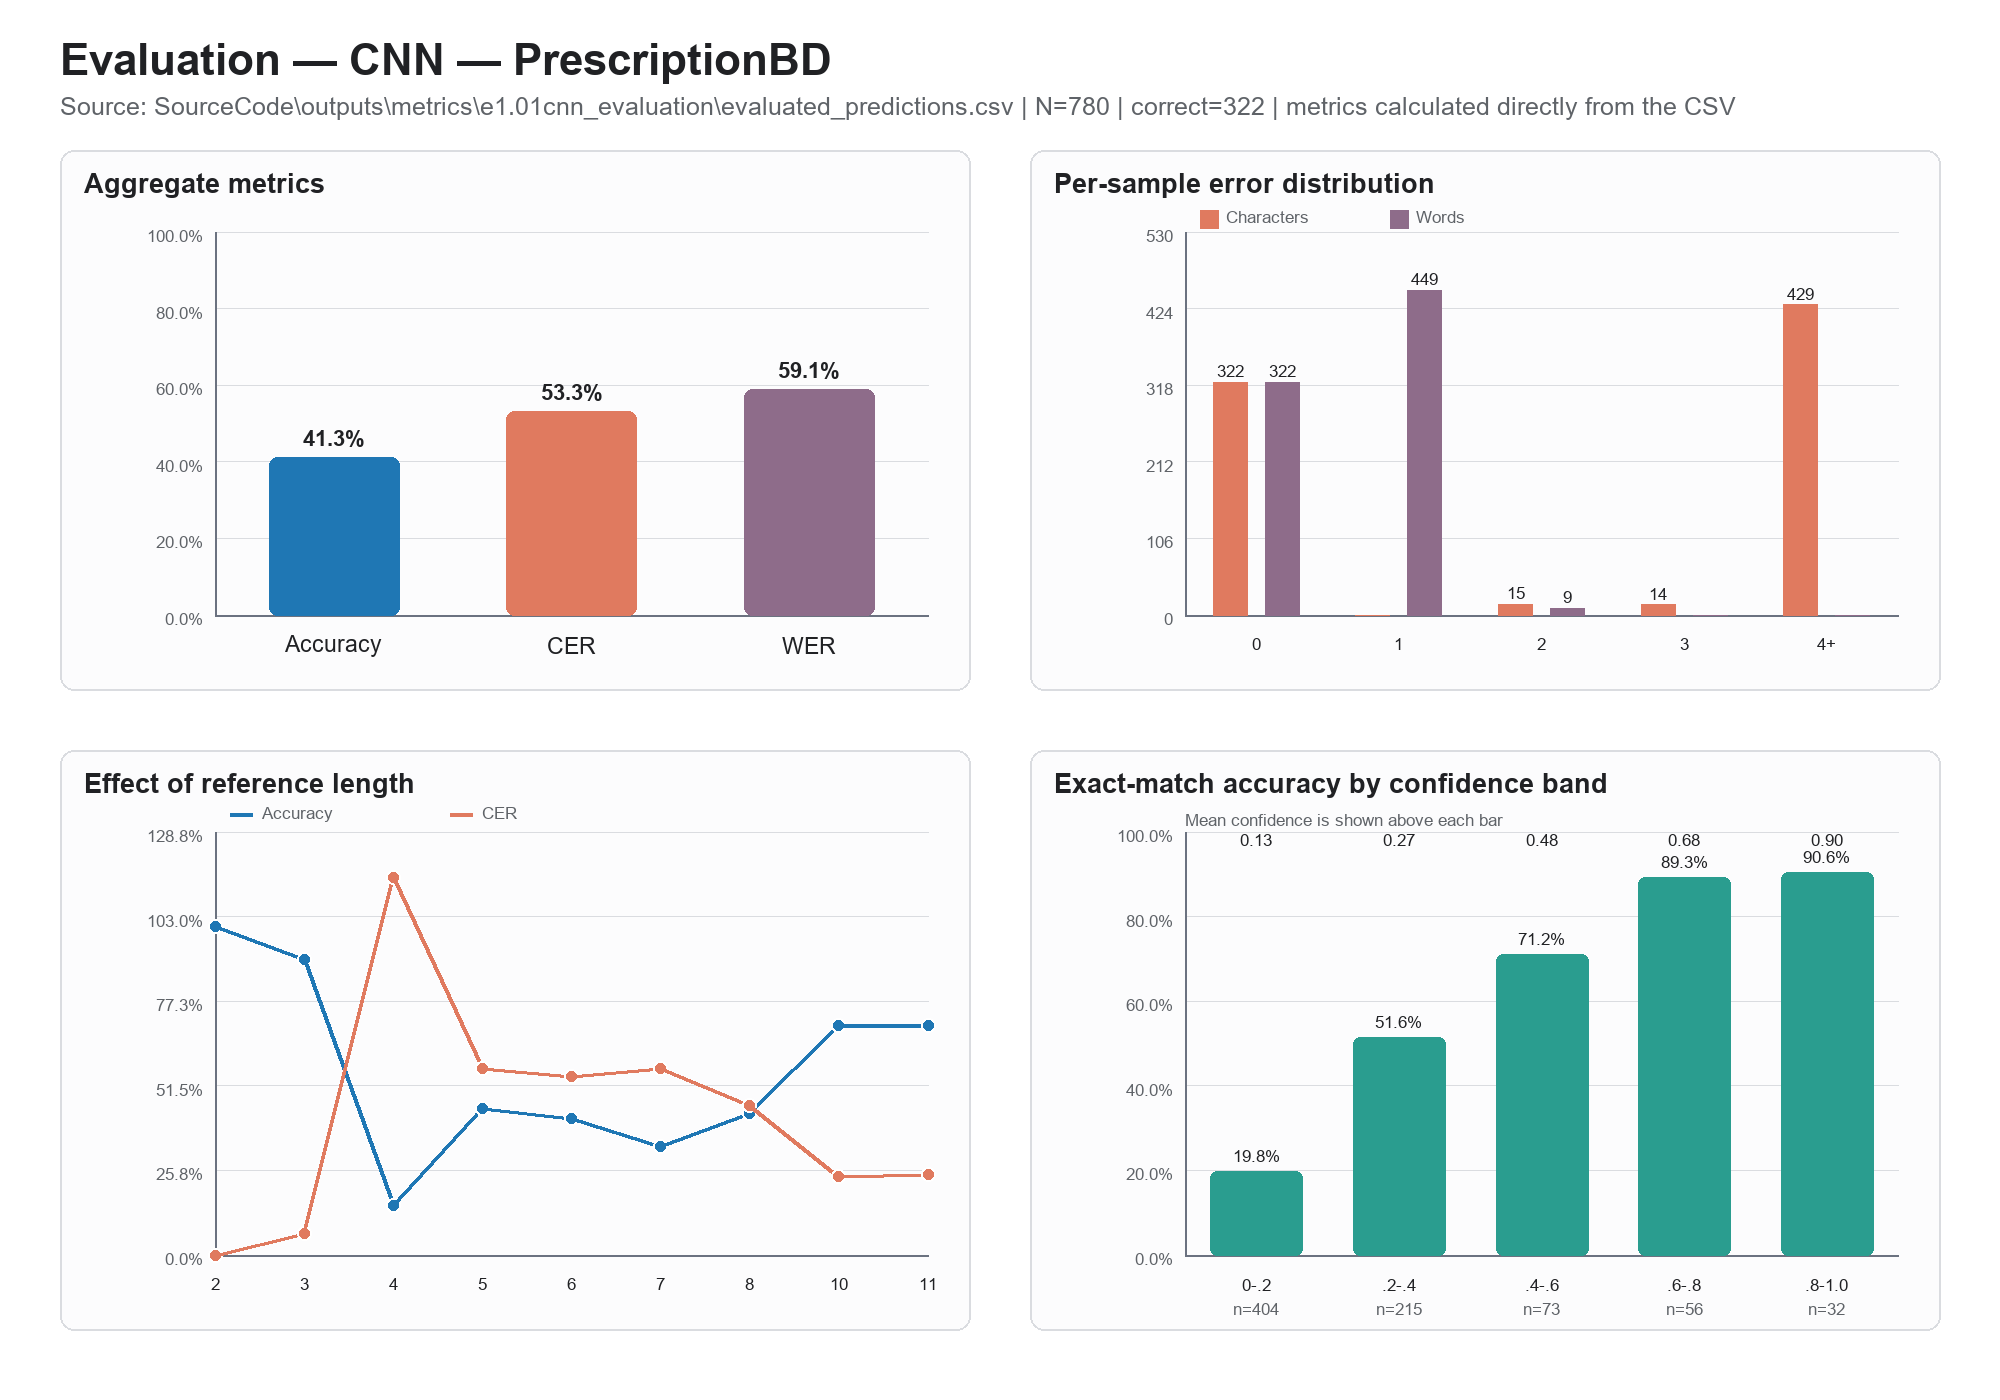
\includegraphics[width=\linewidth]{imagens/evaluation_graficos_tabelas/e1.01cnn_evaluation_evaluated_predictions.png}
    \caption{Evaluated predictions.}
  \end{subfigure}\hfill
  \begin{subfigure}{0.49\linewidth}
    \centering
    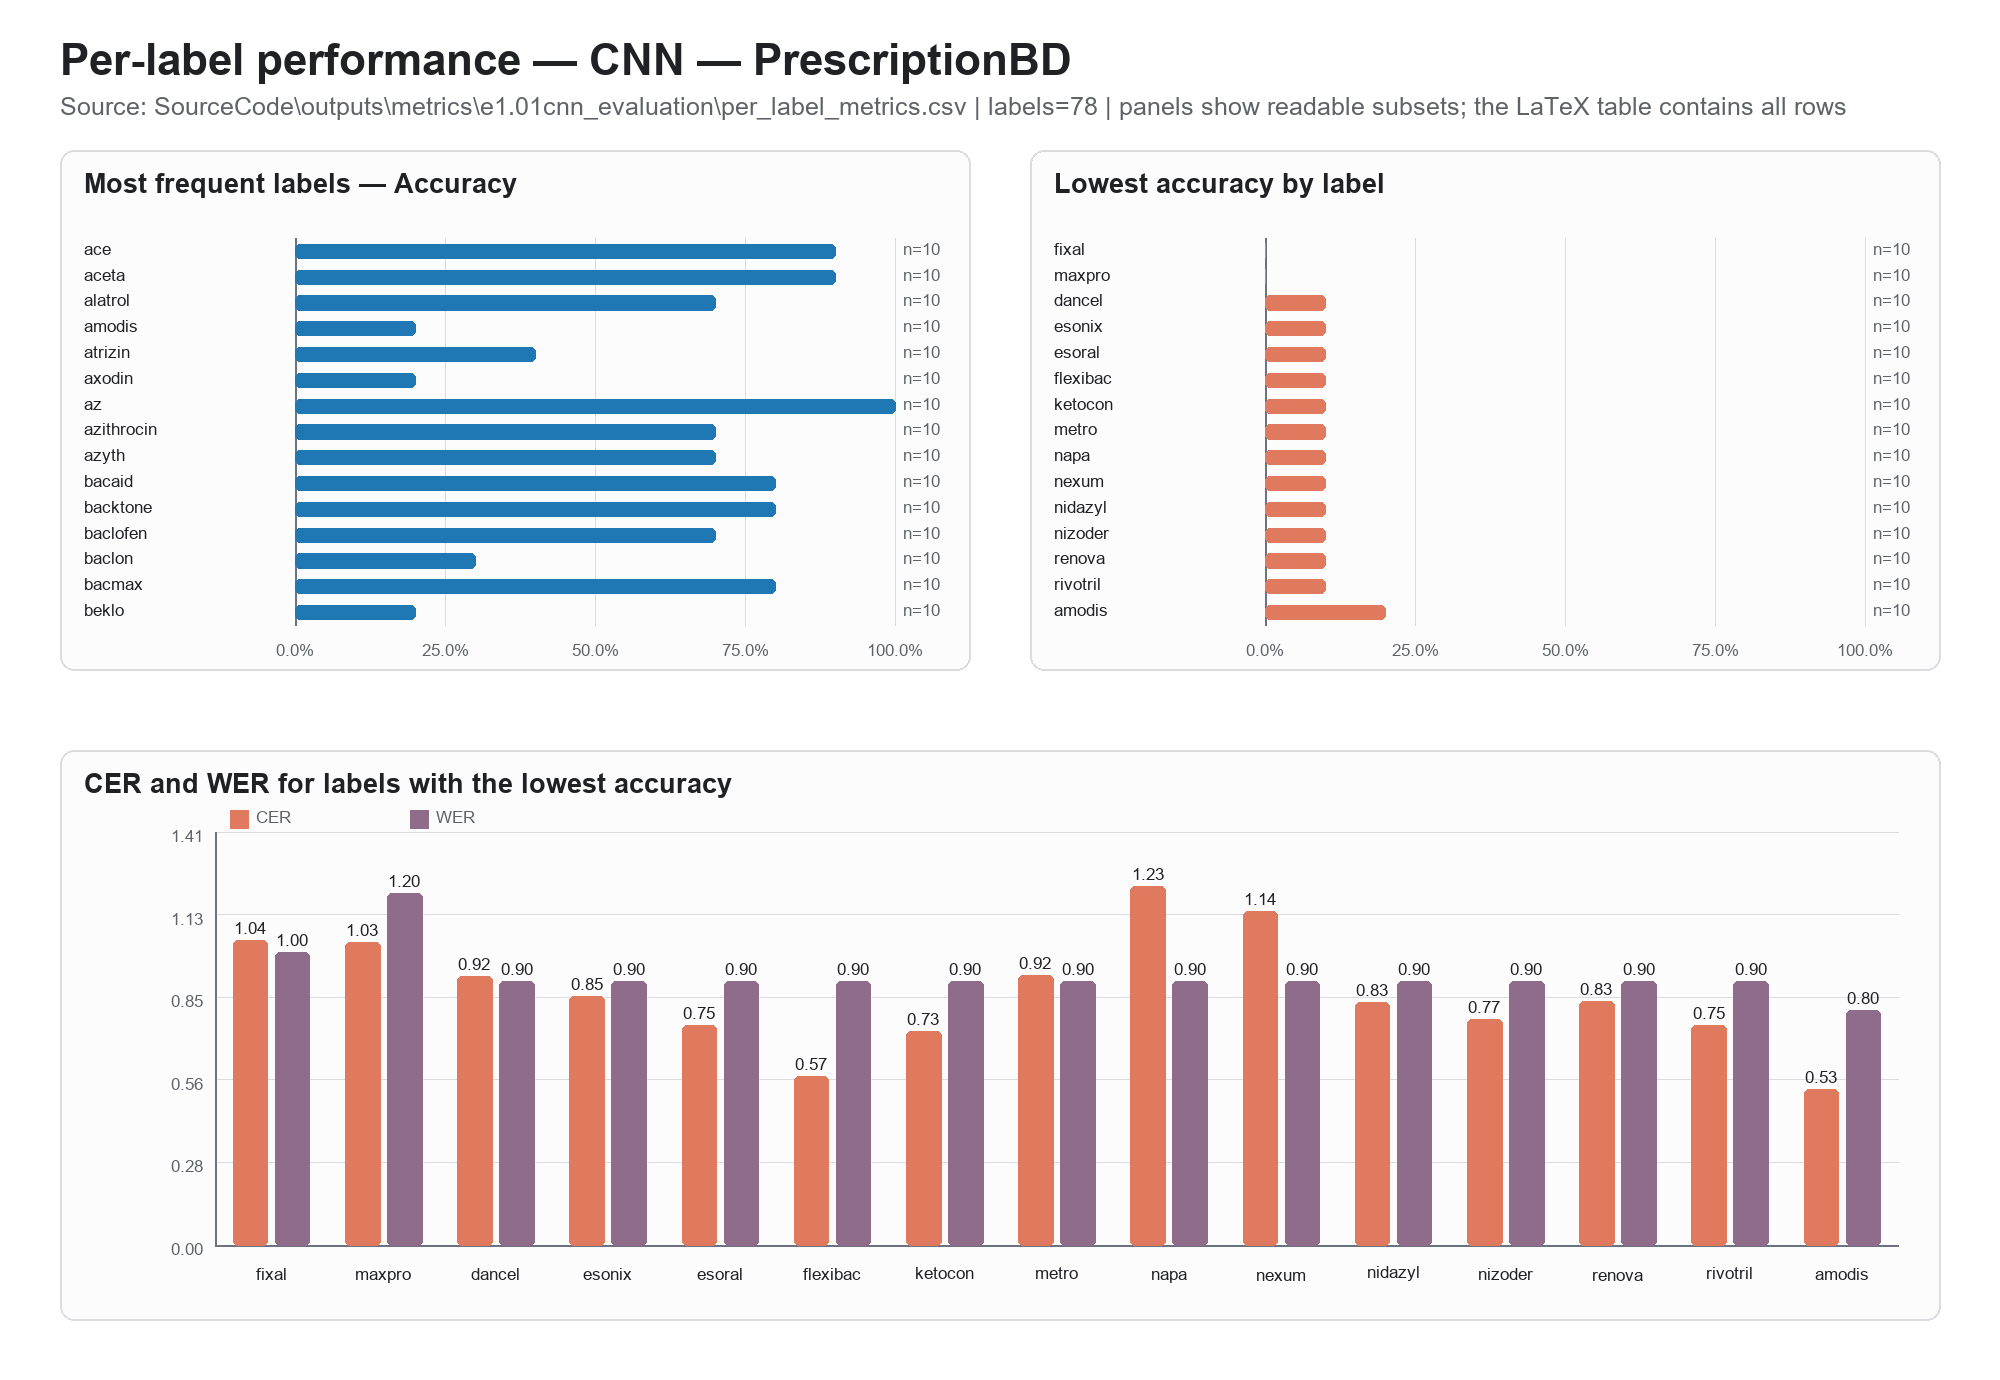
\includegraphics[width=\linewidth]{imagens/evaluation_graficos_tabelas/e1.01cnn_evaluation_per_label_metrics.png}
    \caption{Per-label metrics.}
  \end{subfigure}
  \caption{CNN baseline evaluated on PrescriptionBD.}
  \label{fig:diagnostic-e1-prescriptionbd}
\end{figure}

\begin{figure}[H]
  \centering
  \begin{subfigure}{0.49\linewidth}
    \centering
    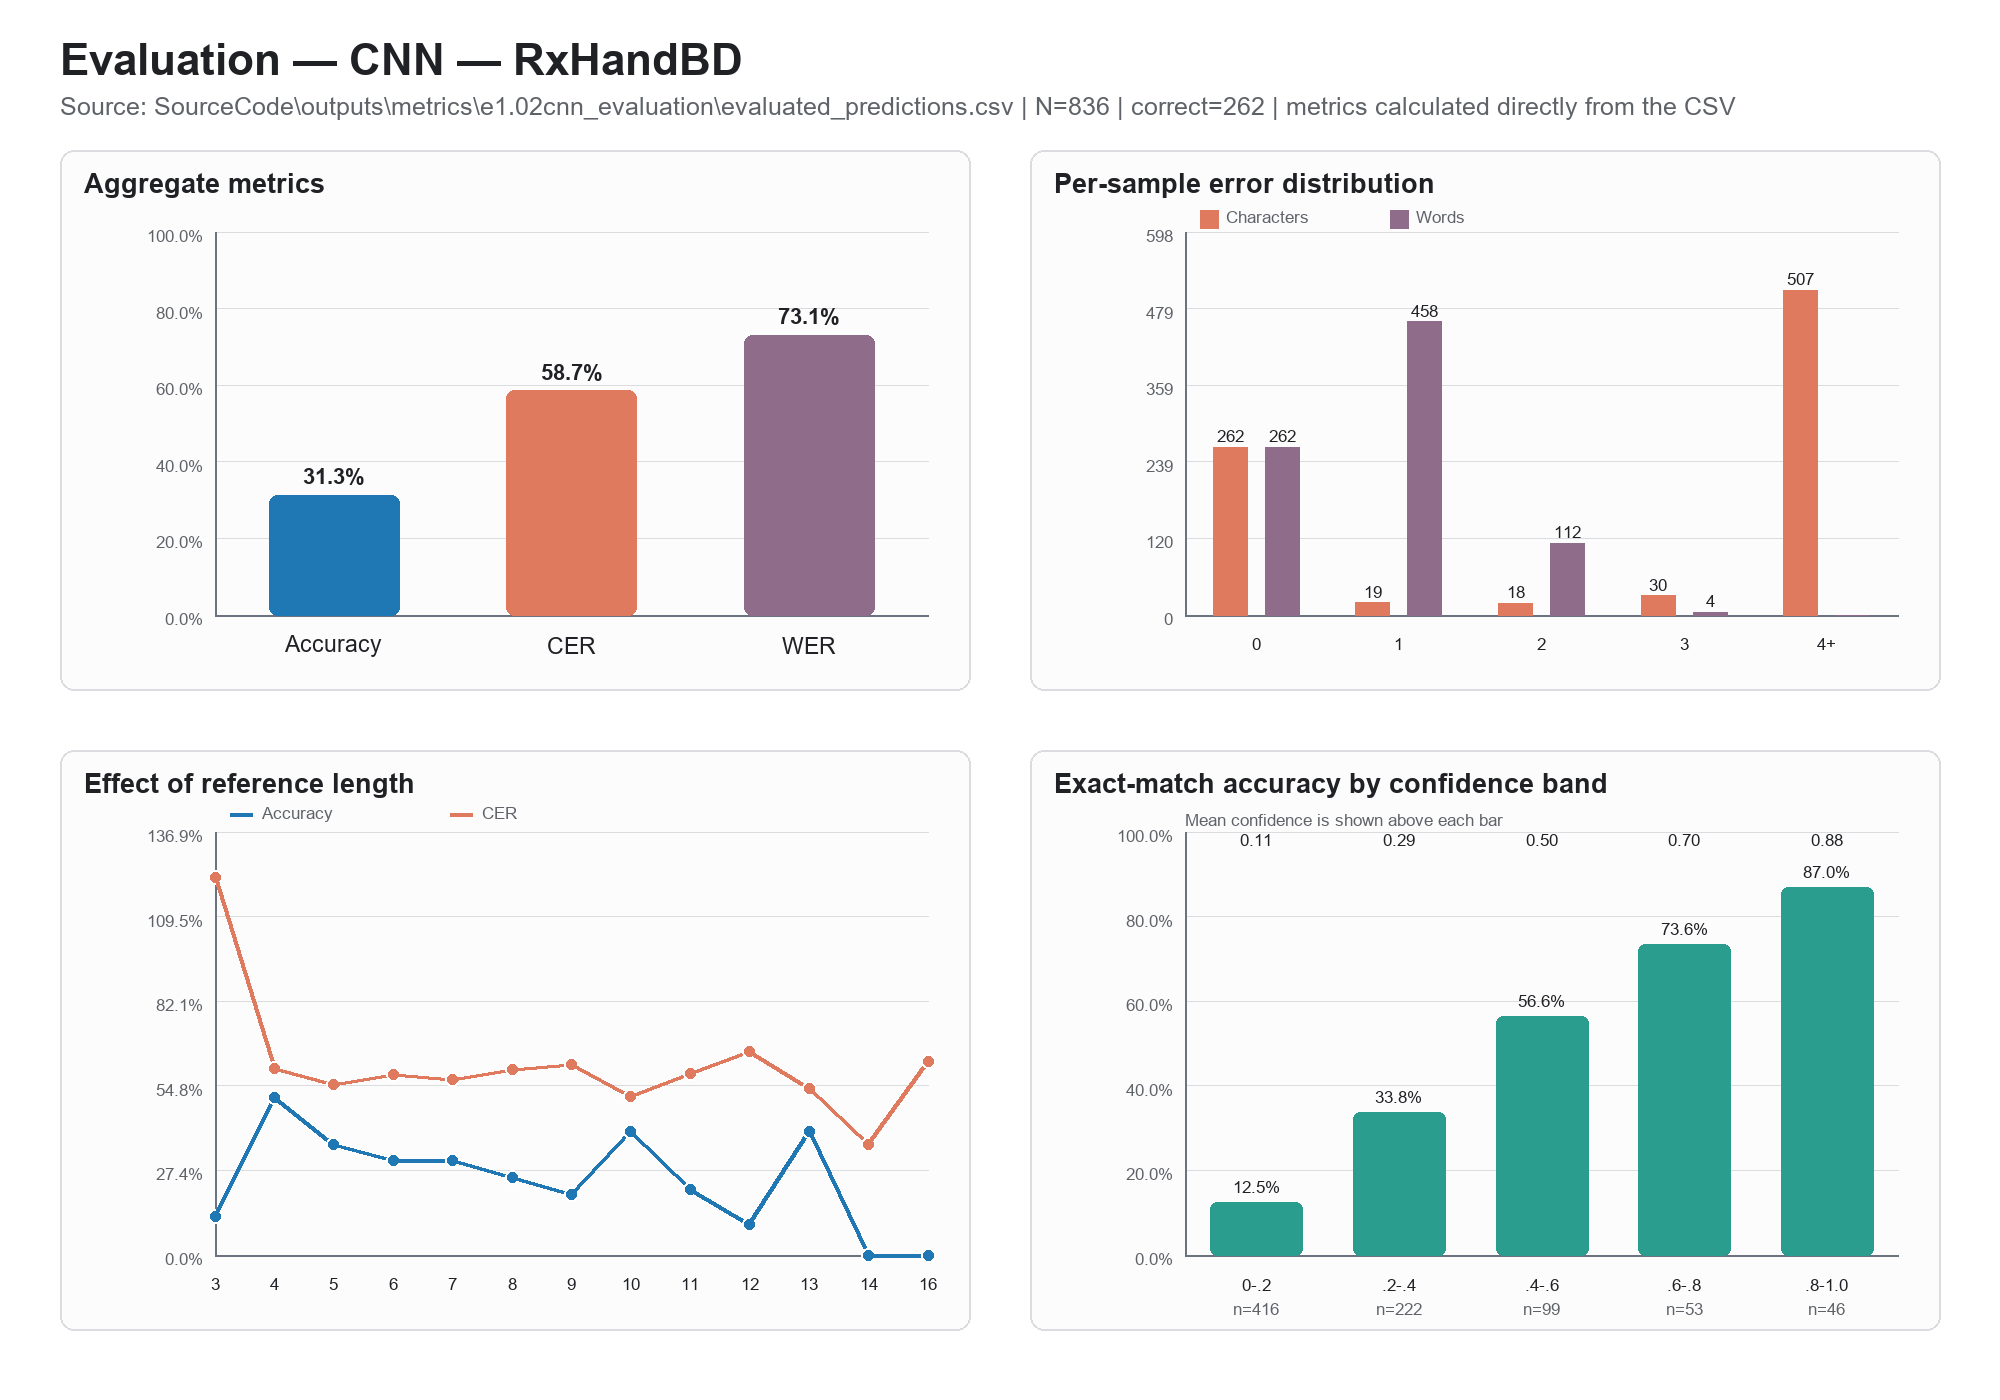
\includegraphics[width=\linewidth]{imagens/evaluation_graficos_tabelas/e1.02cnn_evaluation_evaluated_predictions.png}
    \caption{Evaluated predictions.}
  \end{subfigure}\hfill
  \begin{subfigure}{0.49\linewidth}
    \centering
    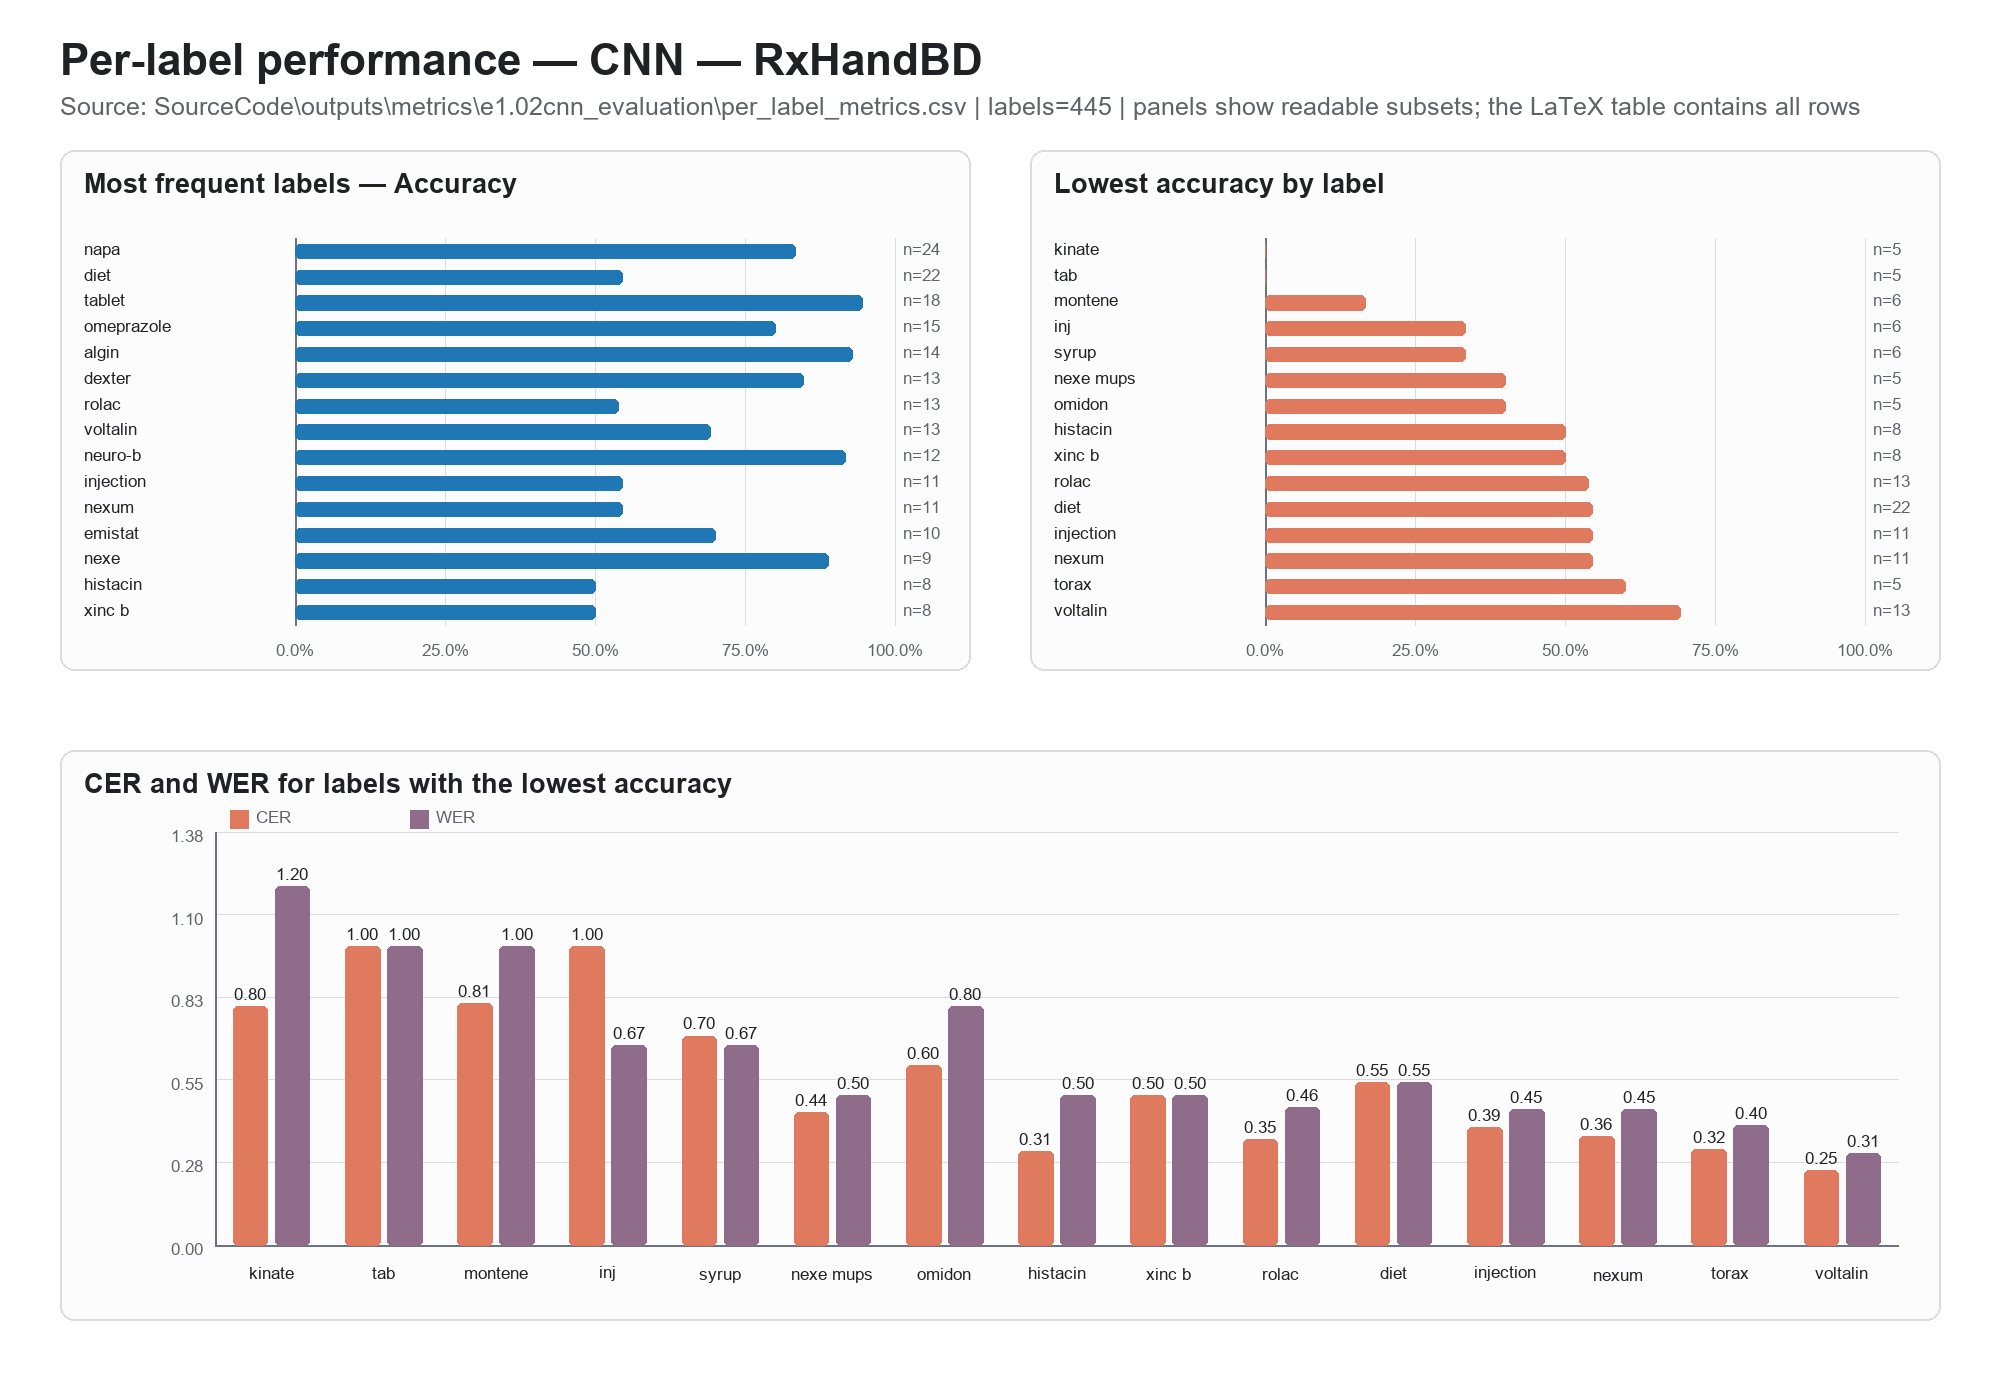
\includegraphics[width=\linewidth]{imagens/evaluation_graficos_tabelas/e1.02cnn_evaluation_per_label_metrics.png}
    \caption{Per-label metrics.}
  \end{subfigure}
  \caption{CNN baseline evaluated on RxHandBD.}
  \label{fig:diagnostic-e1-rxhandbd}
\end{figure}

\begin{figure}[H]
  \centering
  \begin{subfigure}{0.49\linewidth}
    \centering
    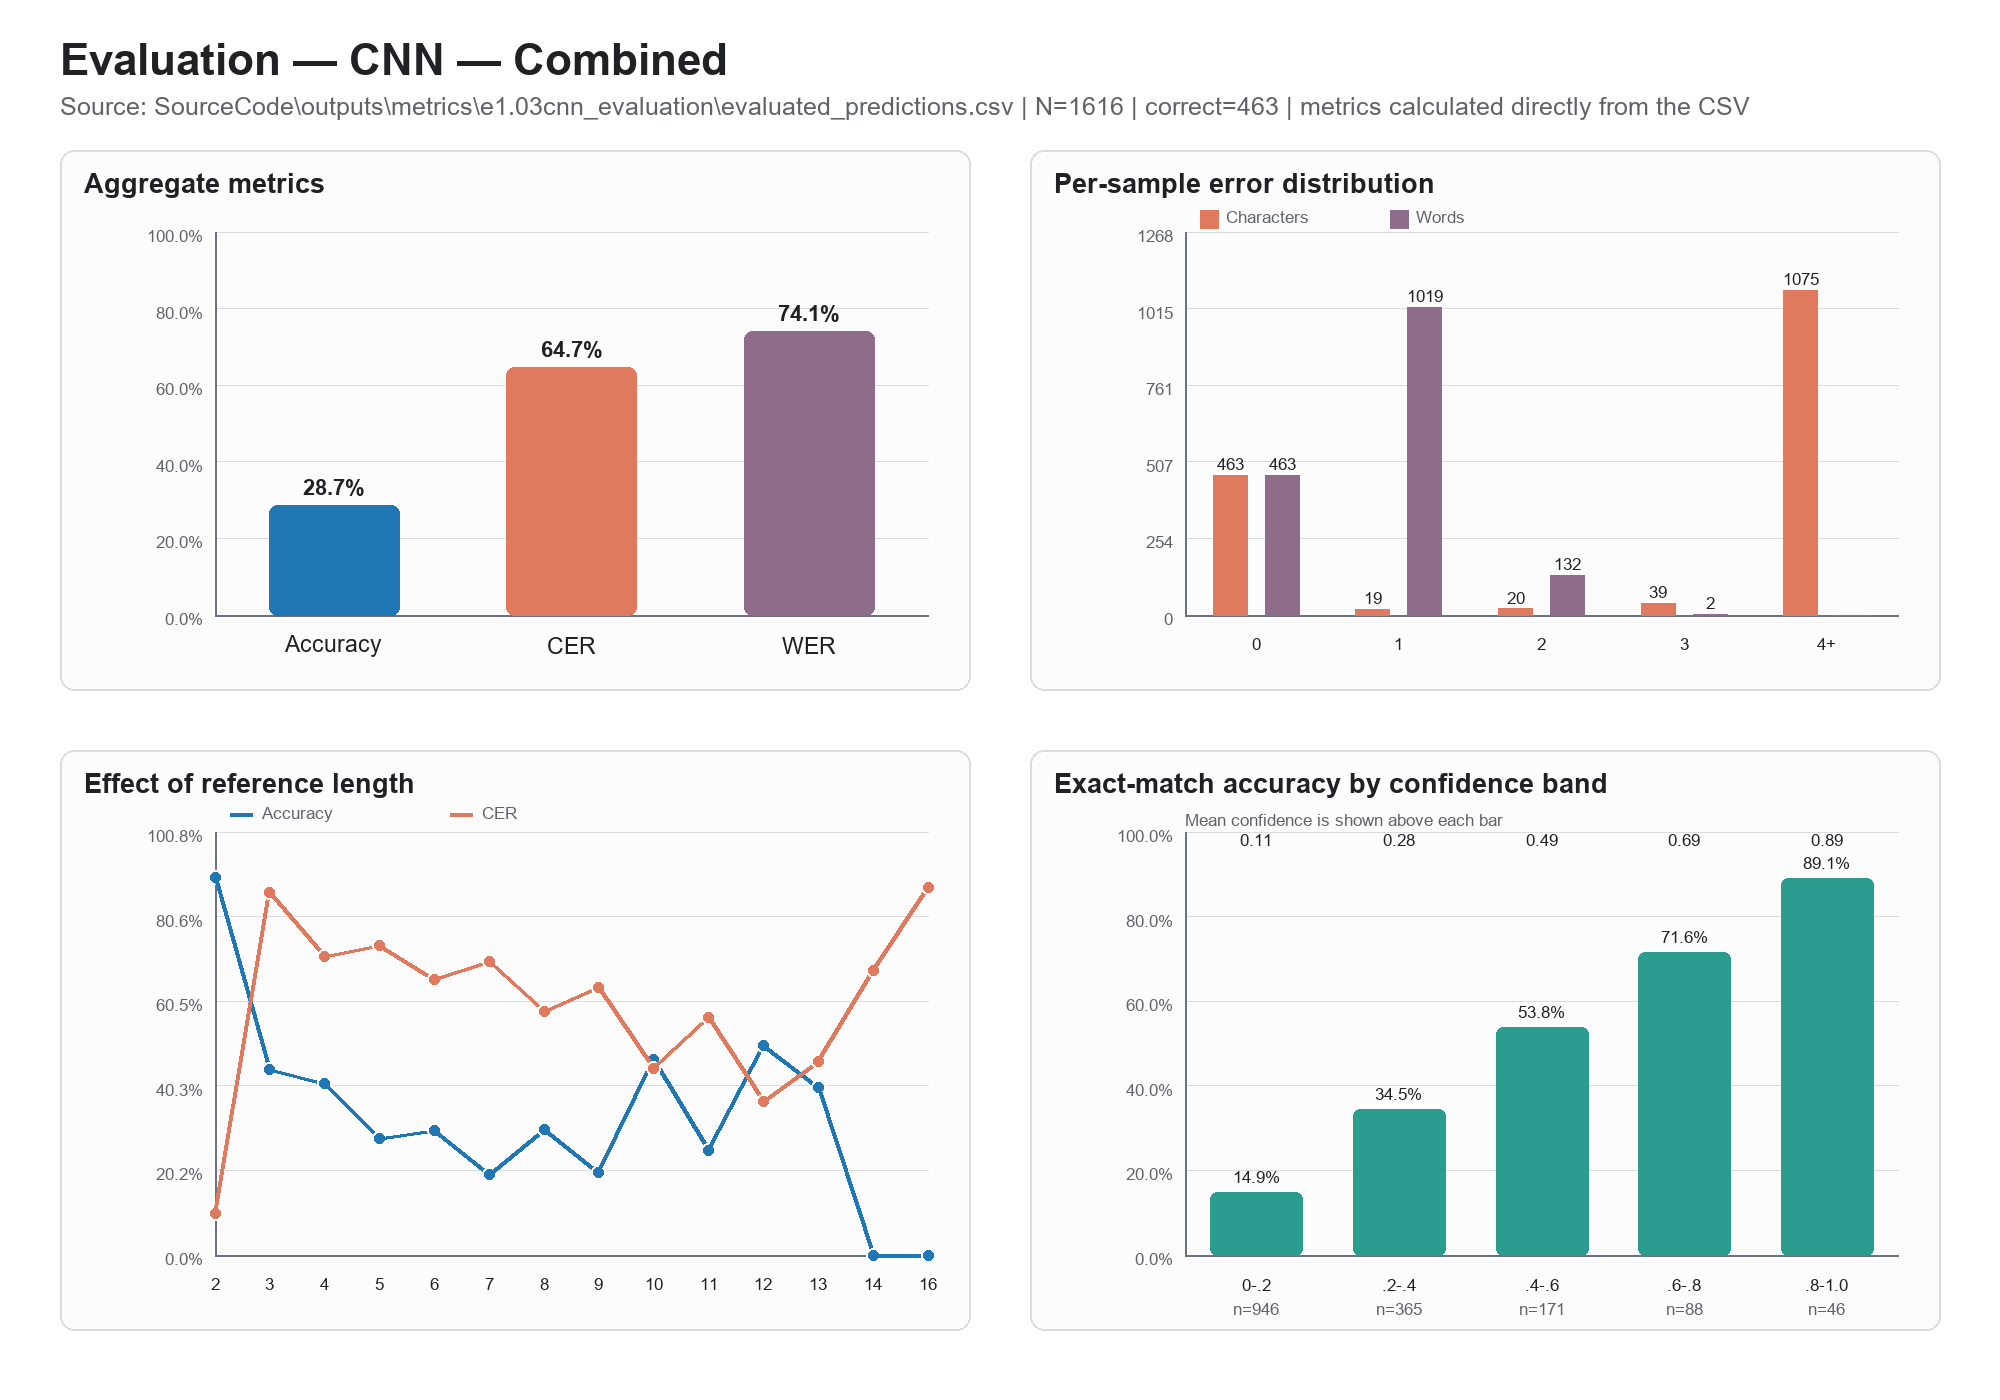
\includegraphics[width=\linewidth]{imagens/evaluation_graficos_tabelas/e1.03cnn_evaluation_evaluated_predictions.png}
    \caption{Evaluated predictions.}
  \end{subfigure}\hfill
  \begin{subfigure}{0.49\linewidth}
    \centering
    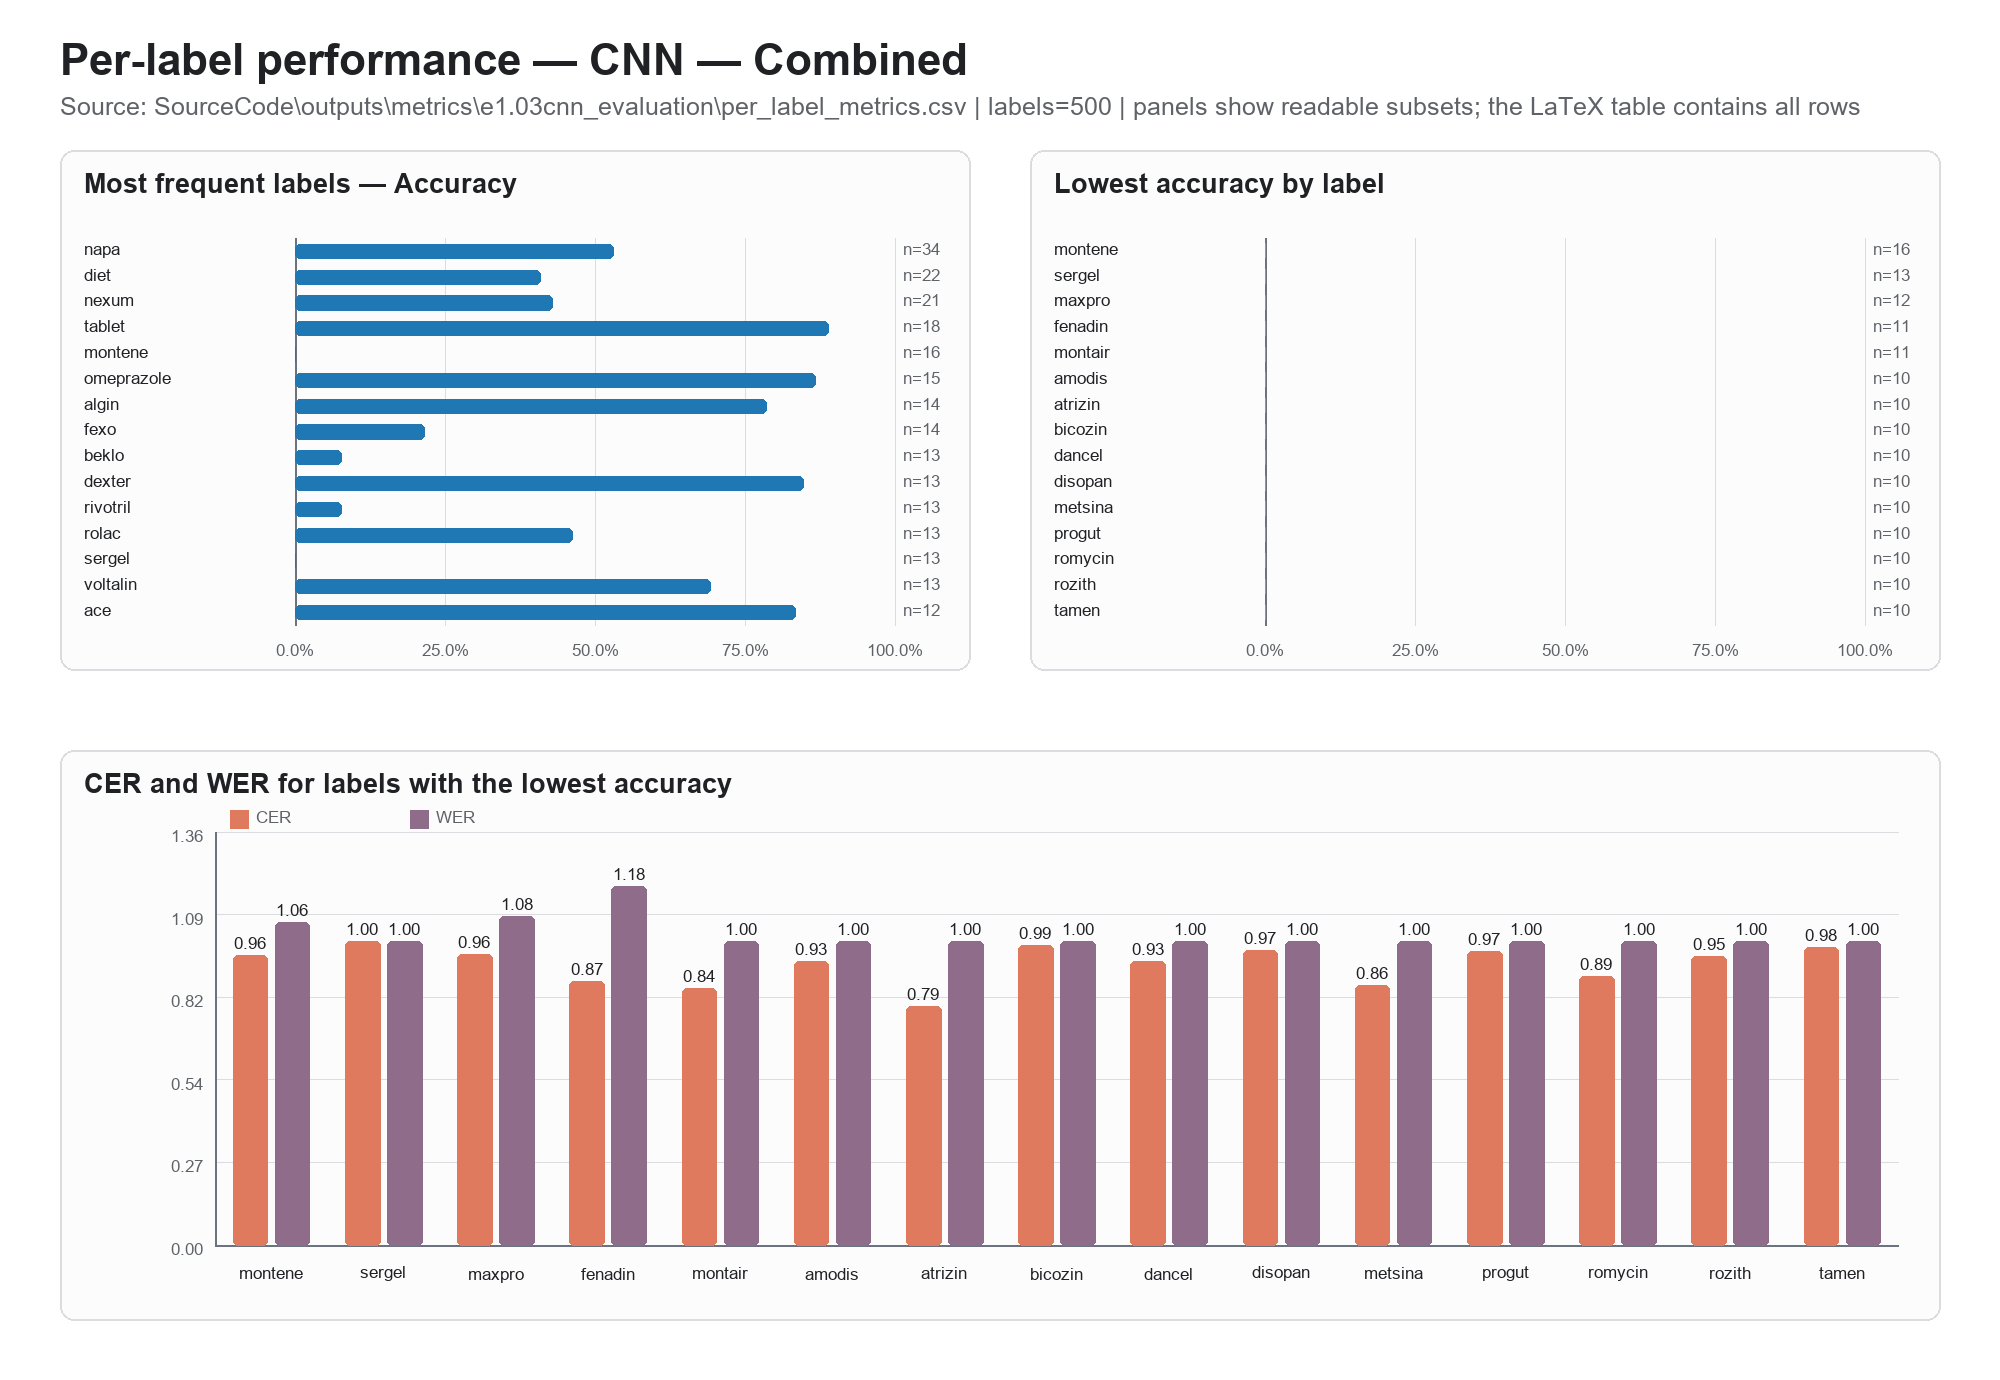
\includegraphics[width=\linewidth]{imagens/evaluation_graficos_tabelas/e1.03cnn_evaluation_per_label_metrics.png}
    \caption{Per-label metrics.}
  \end{subfigure}
  \caption{CNN baseline evaluated in the combined scenario.}
  \label{fig:diagnostic-e1-combined}
\end{figure}

\subsubsection{CNN-BiLSTM}

\begin{figure}[H]
  \centering
  \begin{subfigure}{0.49\linewidth}
    \centering
    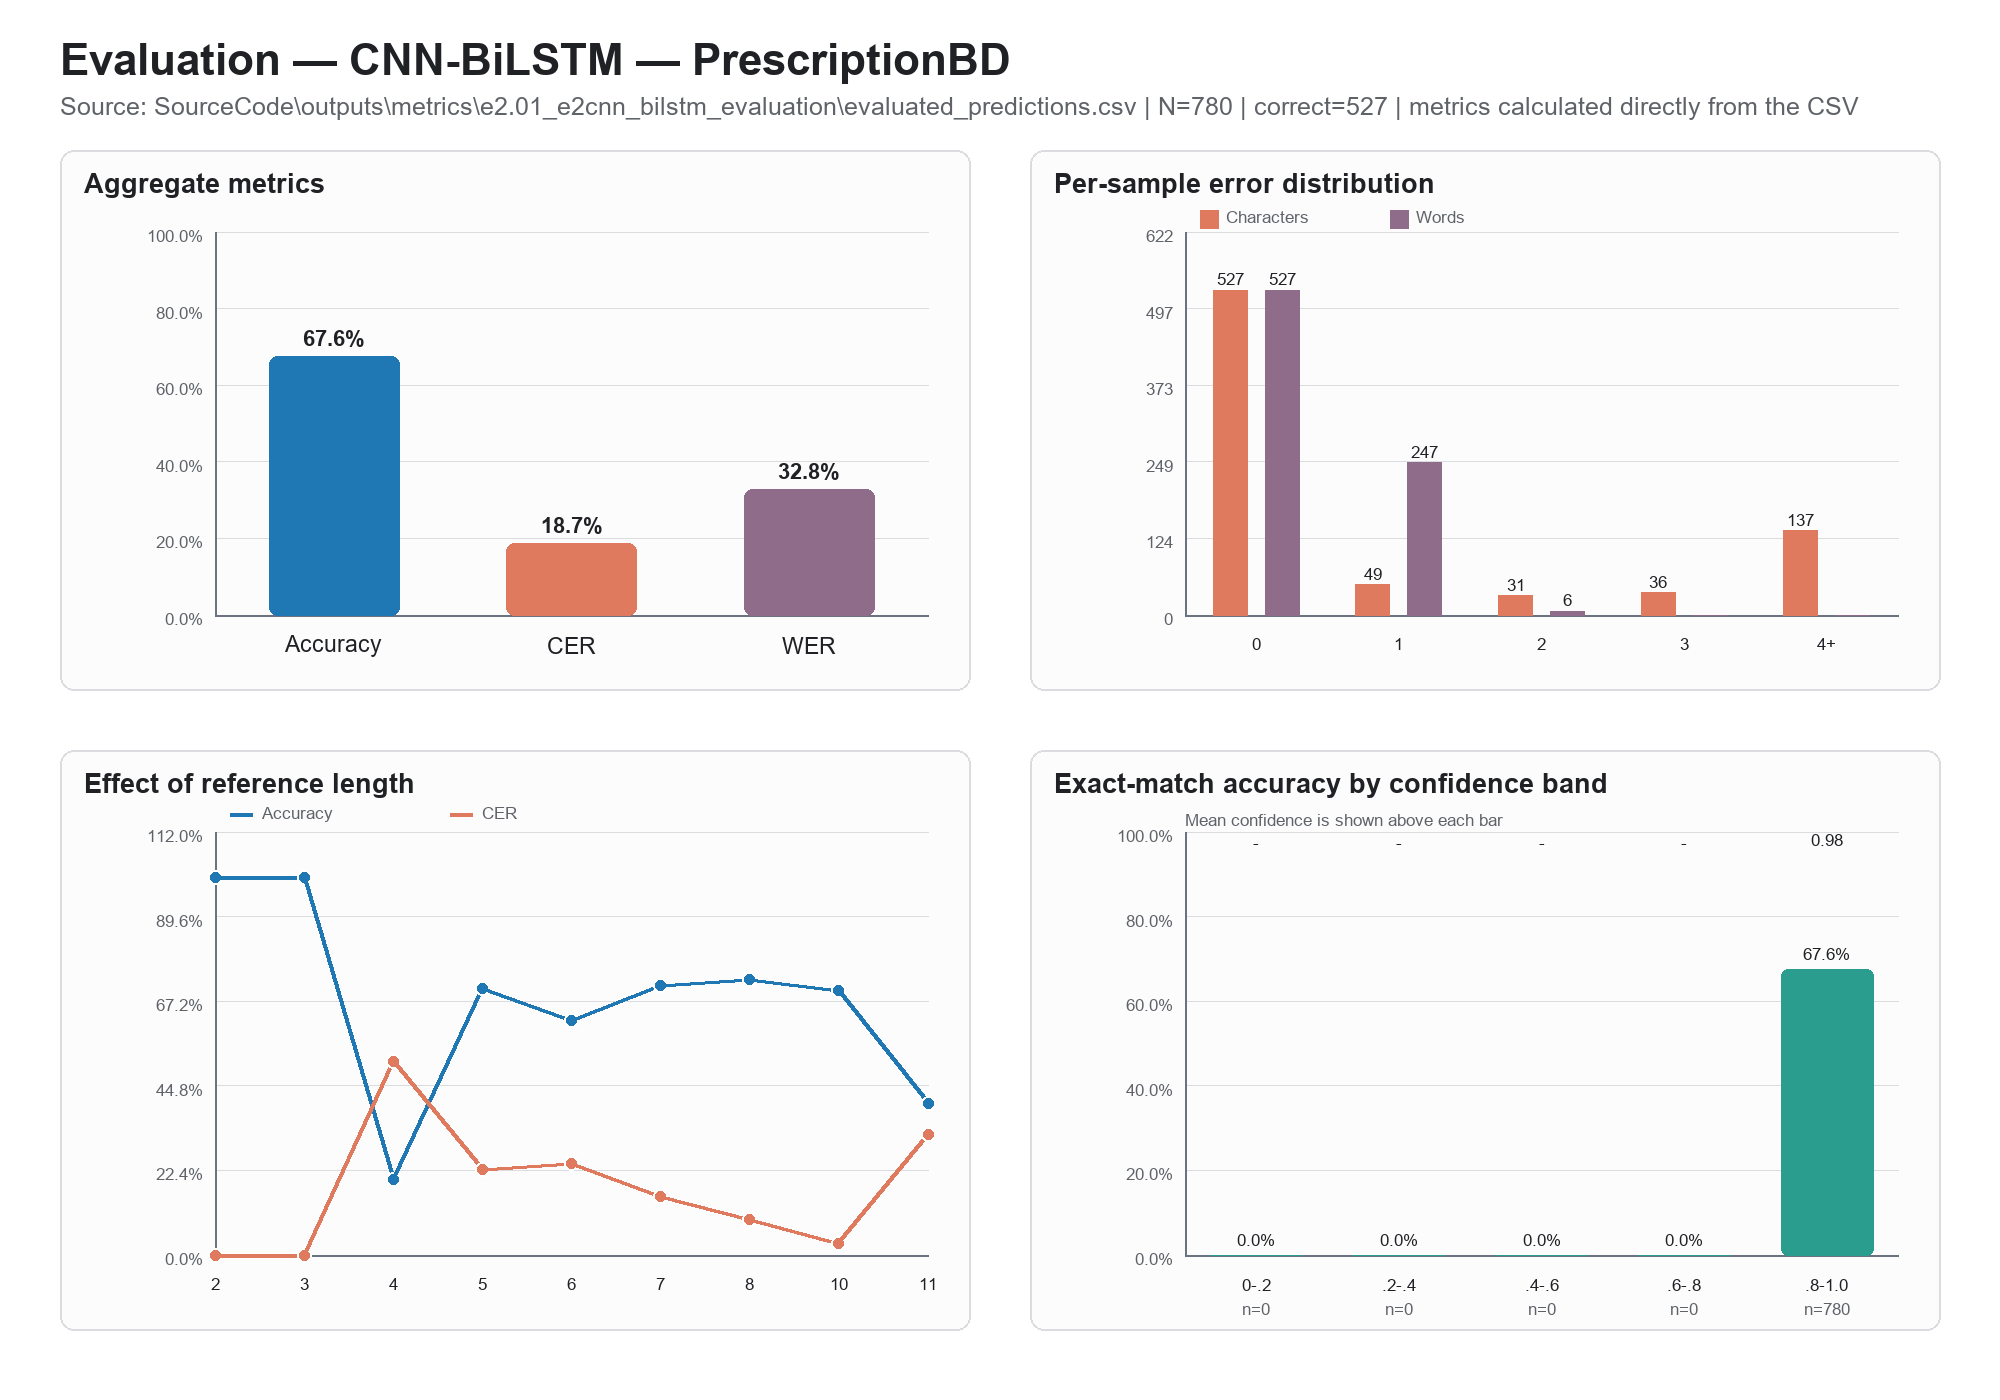
\includegraphics[width=\linewidth]{imagens/evaluation_graficos_tabelas/e2.01_e2cnn_bilstm_evaluation_evaluated_predictions.png}
    \caption{Evaluated predictions.}
  \end{subfigure}\hfill
  \begin{subfigure}{0.49\linewidth}
    \centering
    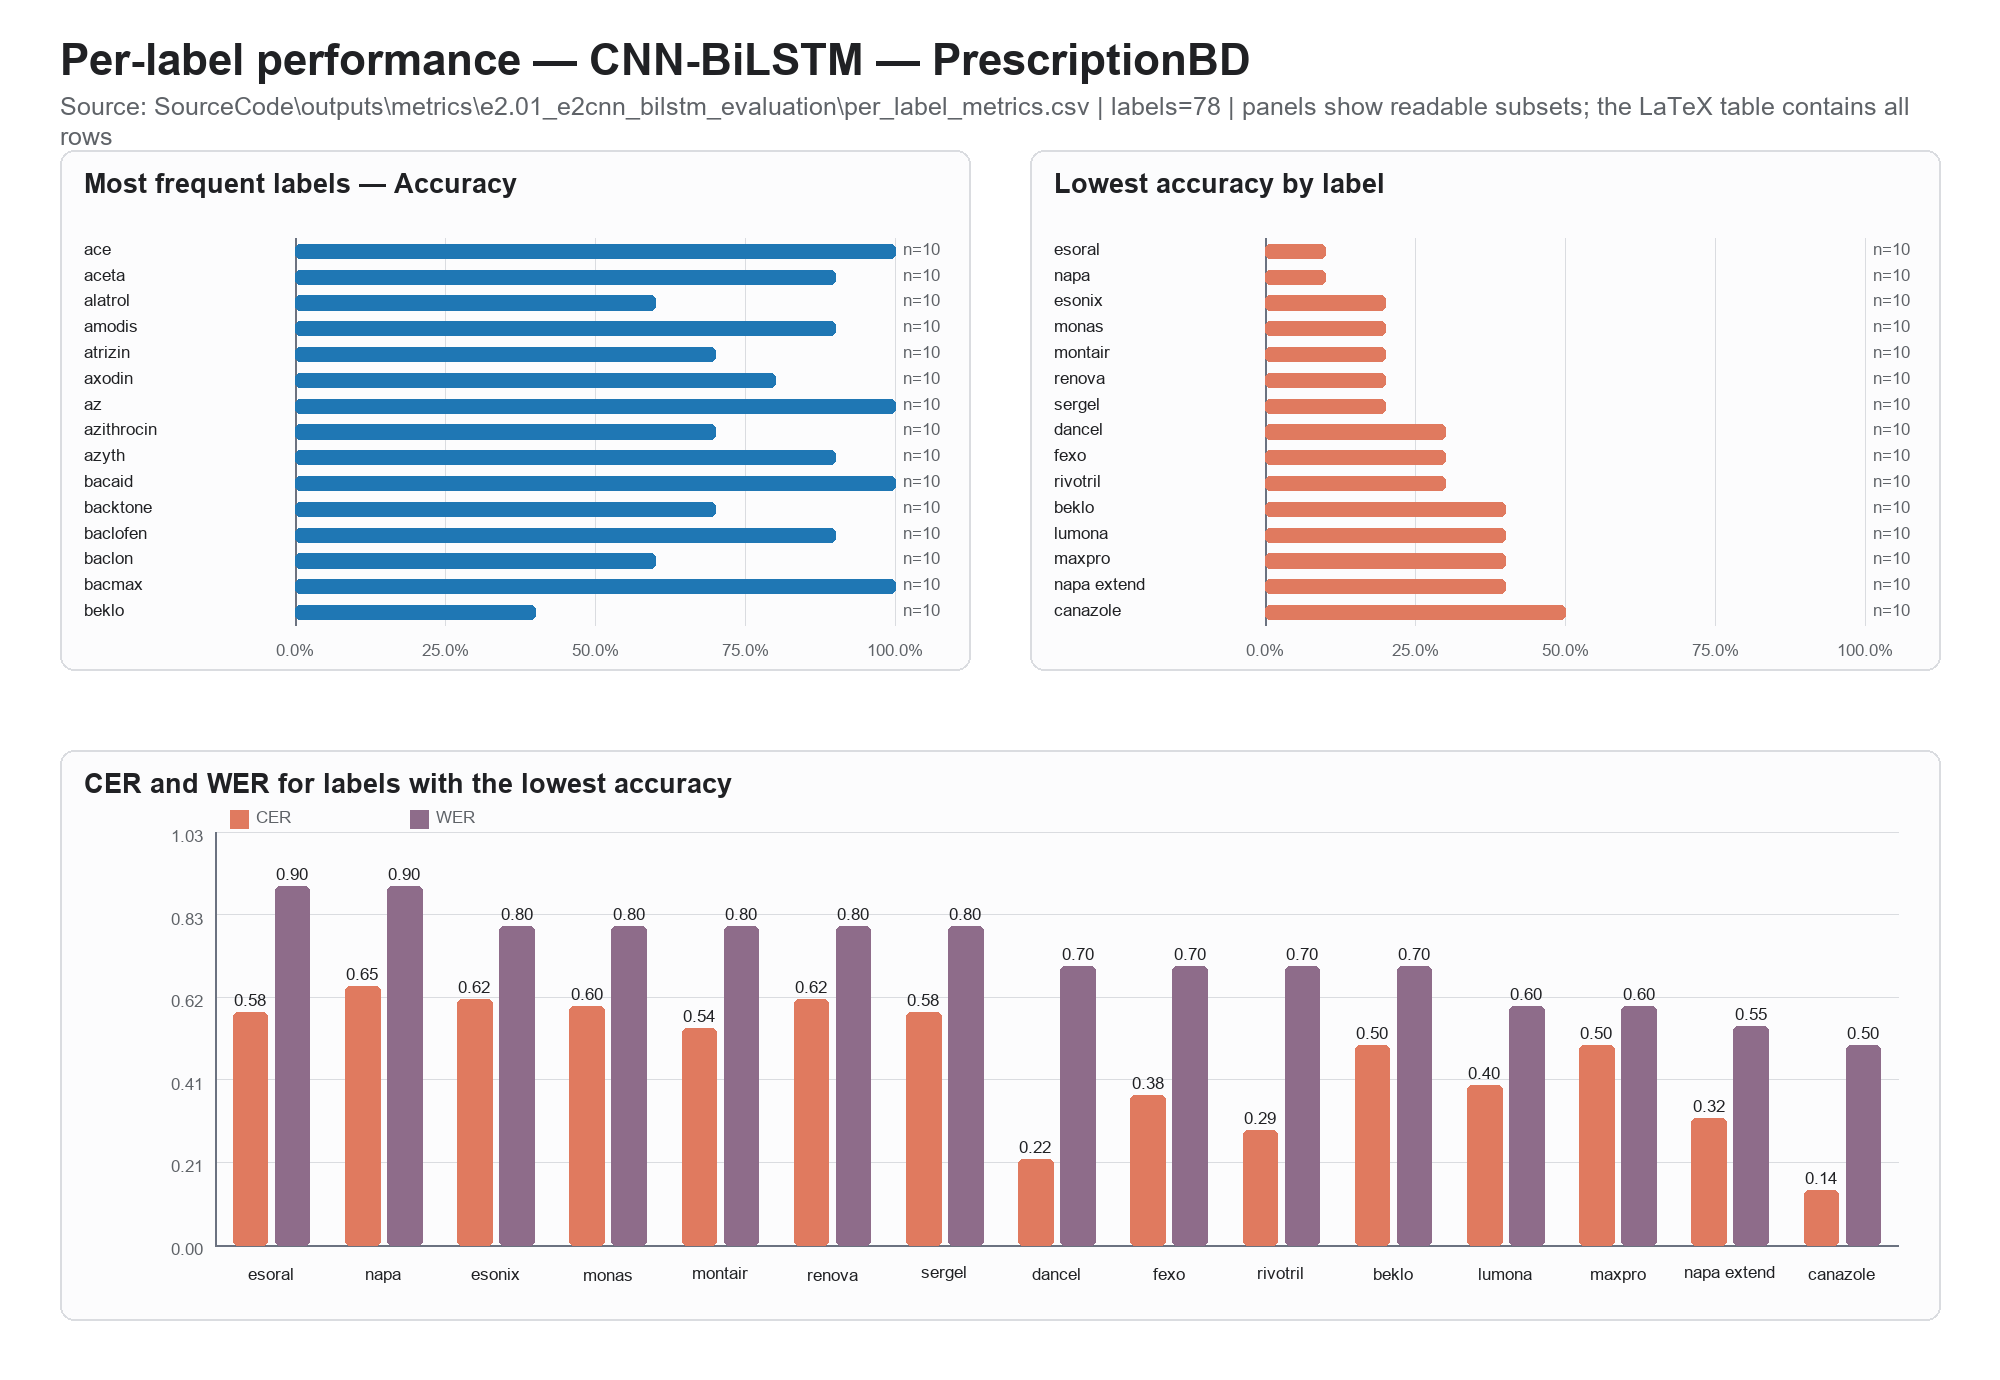
\includegraphics[width=\linewidth]{imagens/evaluation_graficos_tabelas/e2.01_e2cnn_bilstm_evaluation_per_label_metrics.png}
    \caption{Per-label metrics.}
  \end{subfigure}
  \caption{CNN-BiLSTM evaluated on PrescriptionBD.}
  \label{fig:diagnostic-e2-prescriptionbd}
\end{figure}

\begin{figure}[H]
  \centering
  \begin{subfigure}{0.49\linewidth}
    \centering
    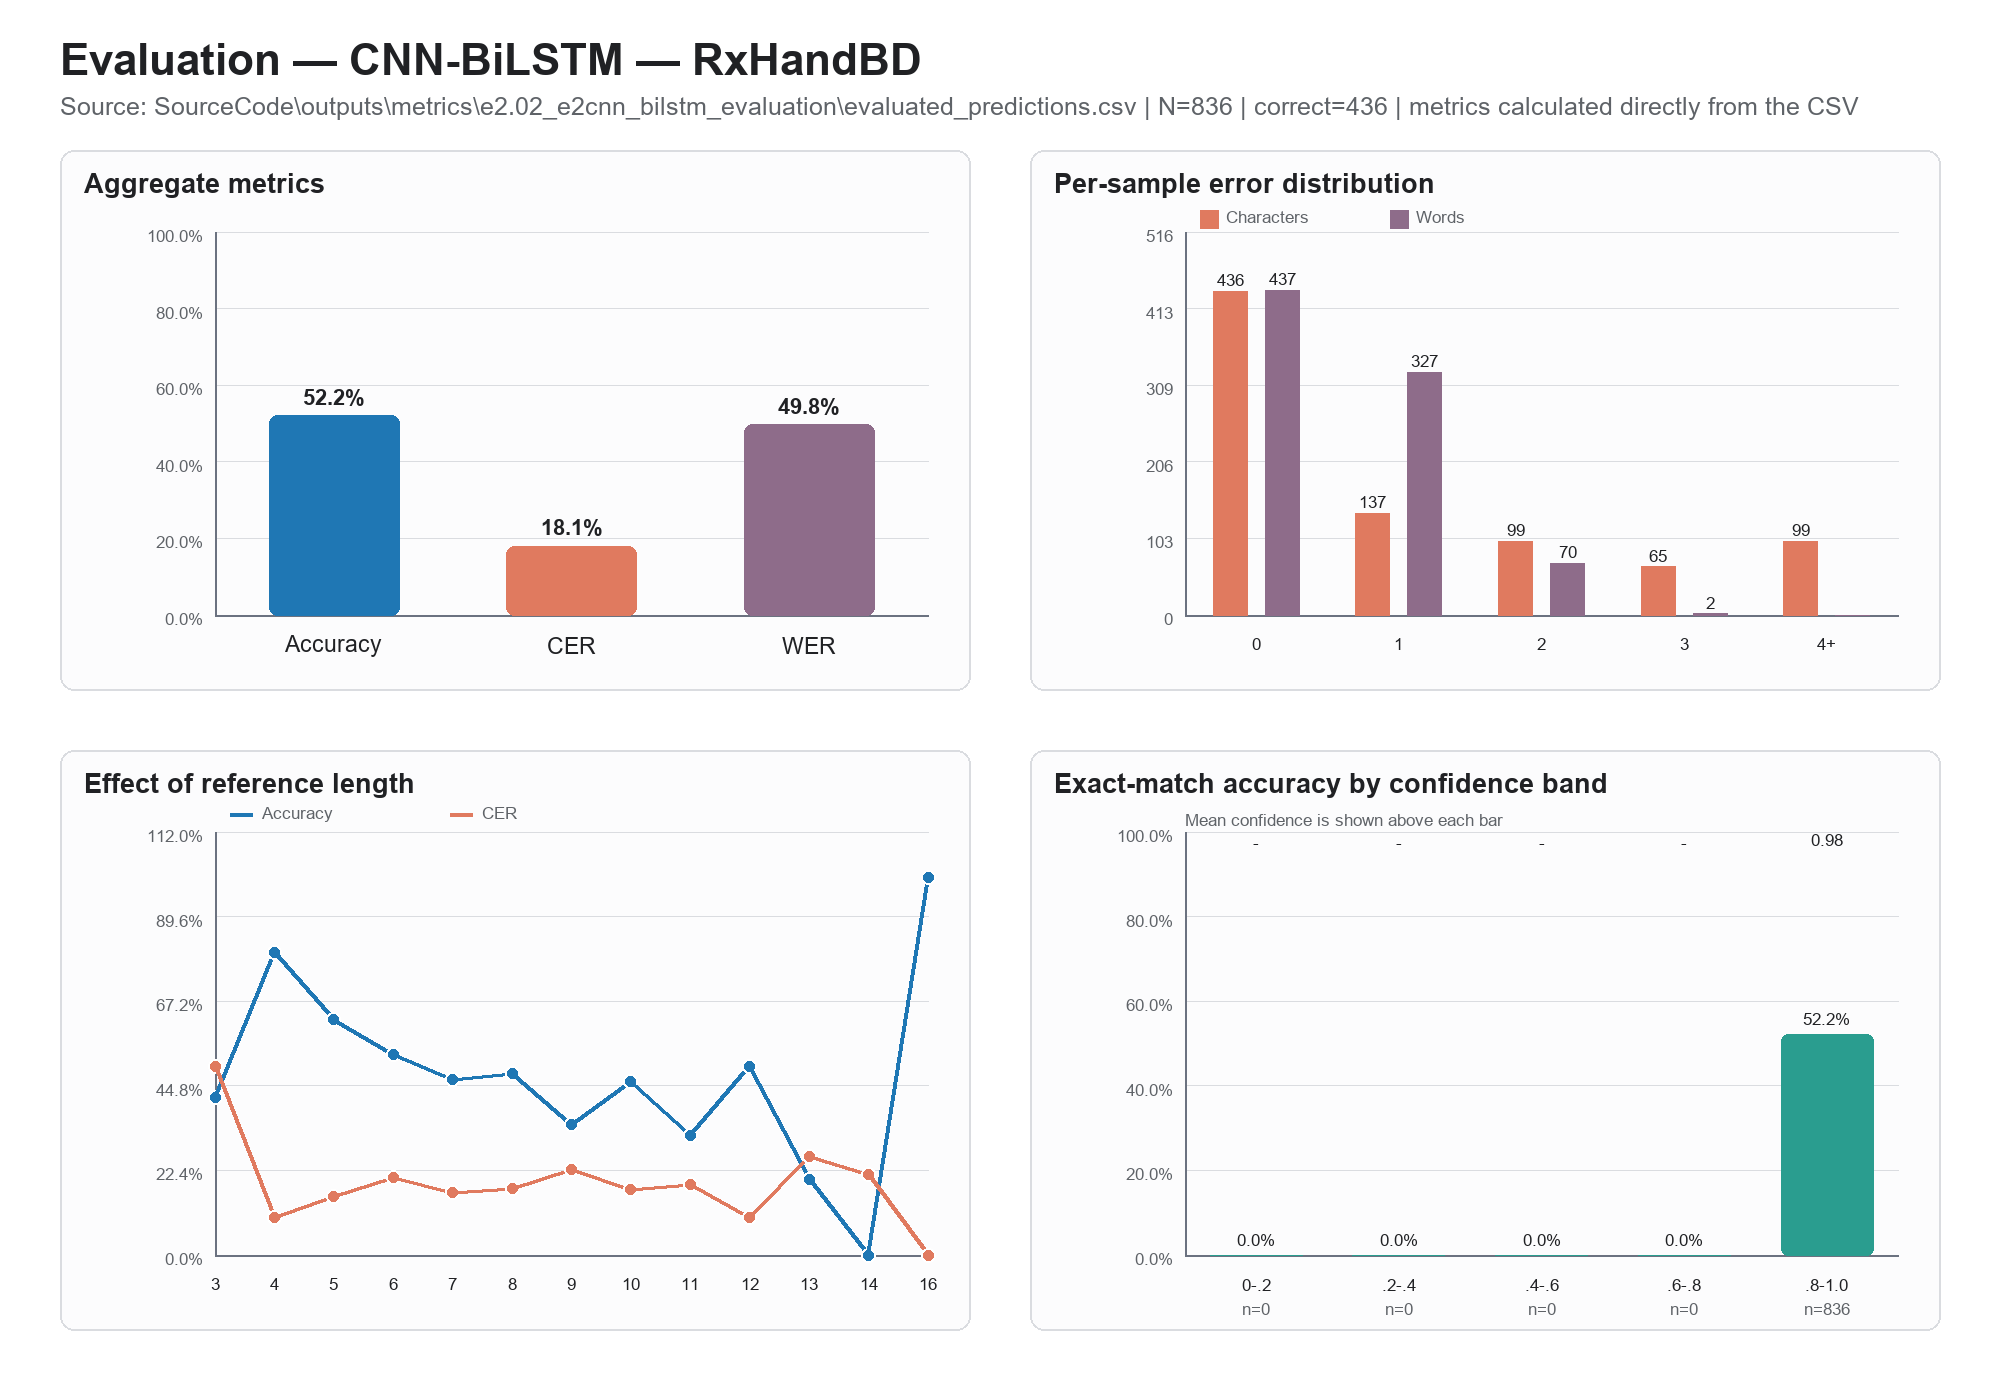
\includegraphics[width=\linewidth]{imagens/evaluation_graficos_tabelas/e2.02_e2cnn_bilstm_evaluation_evaluated_predictions.png}
    \caption{Evaluated predictions.}
  \end{subfigure}\hfill
  \begin{subfigure}{0.49\linewidth}
    \centering
    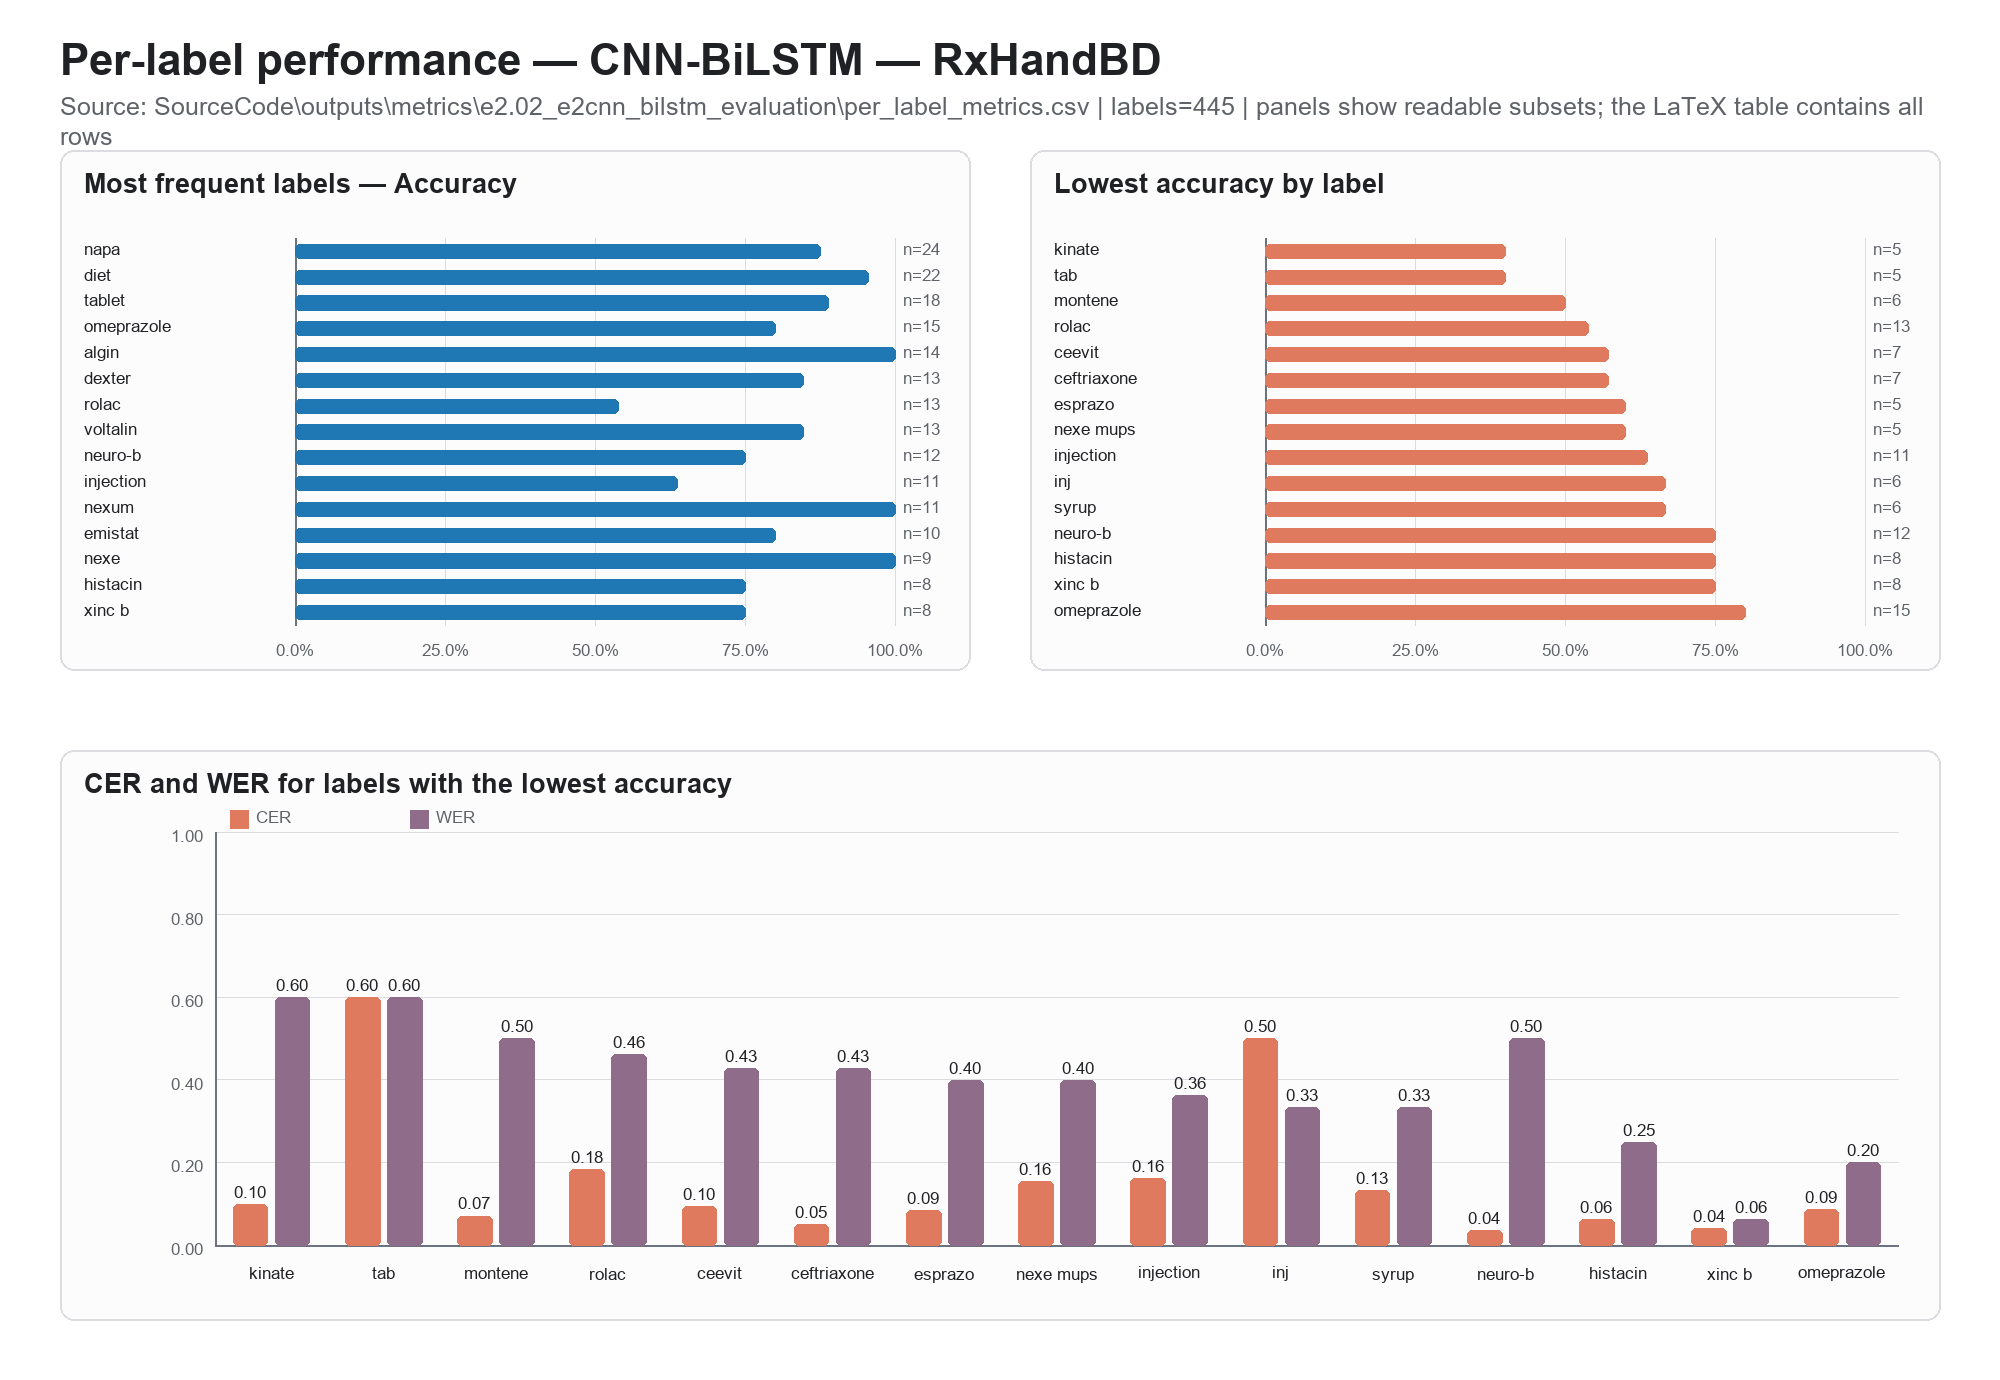
\includegraphics[width=\linewidth]{imagens/evaluation_graficos_tabelas/e2.02_e2cnn_bilstm_evaluation_per_label_metrics.png}
    \caption{Per-label metrics.}
  \end{subfigure}
  \caption{CNN-BiLSTM evaluated on RxHandBD.}
  \label{fig:diagnostic-e2-rxhandbd}
\end{figure}

\begin{figure}[H]
  \centering
  \begin{subfigure}{0.49\linewidth}
    \centering
    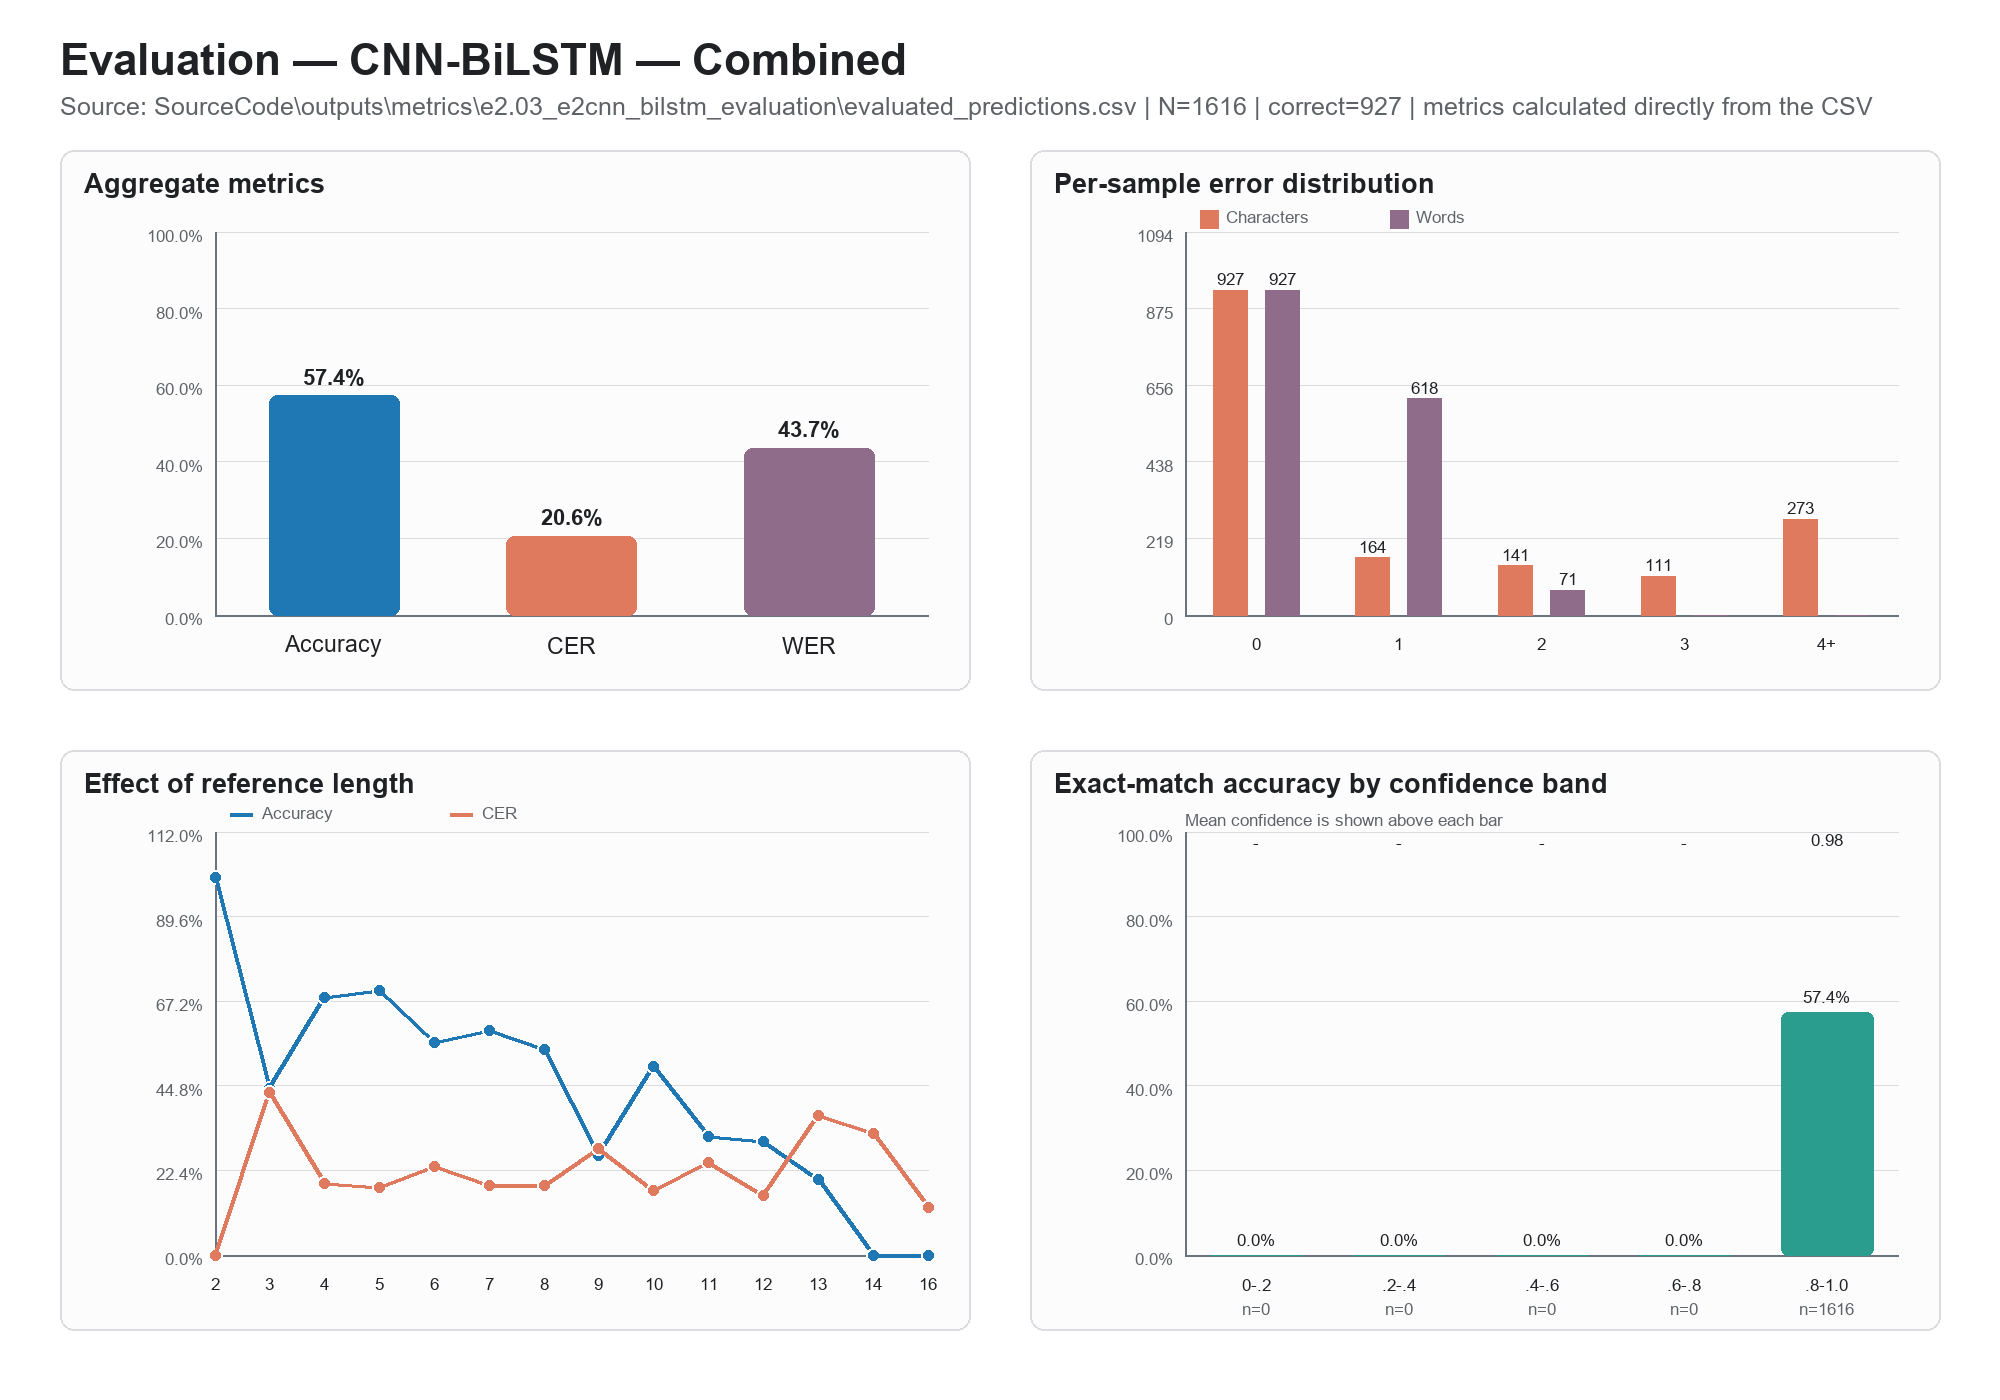
\includegraphics[width=\linewidth]{imagens/evaluation_graficos_tabelas/e2.03_e2cnn_bilstm_evaluation_evaluated_predictions.png}
    \caption{Evaluated predictions.}
  \end{subfigure}\hfill
  \begin{subfigure}{0.49\linewidth}
    \centering
    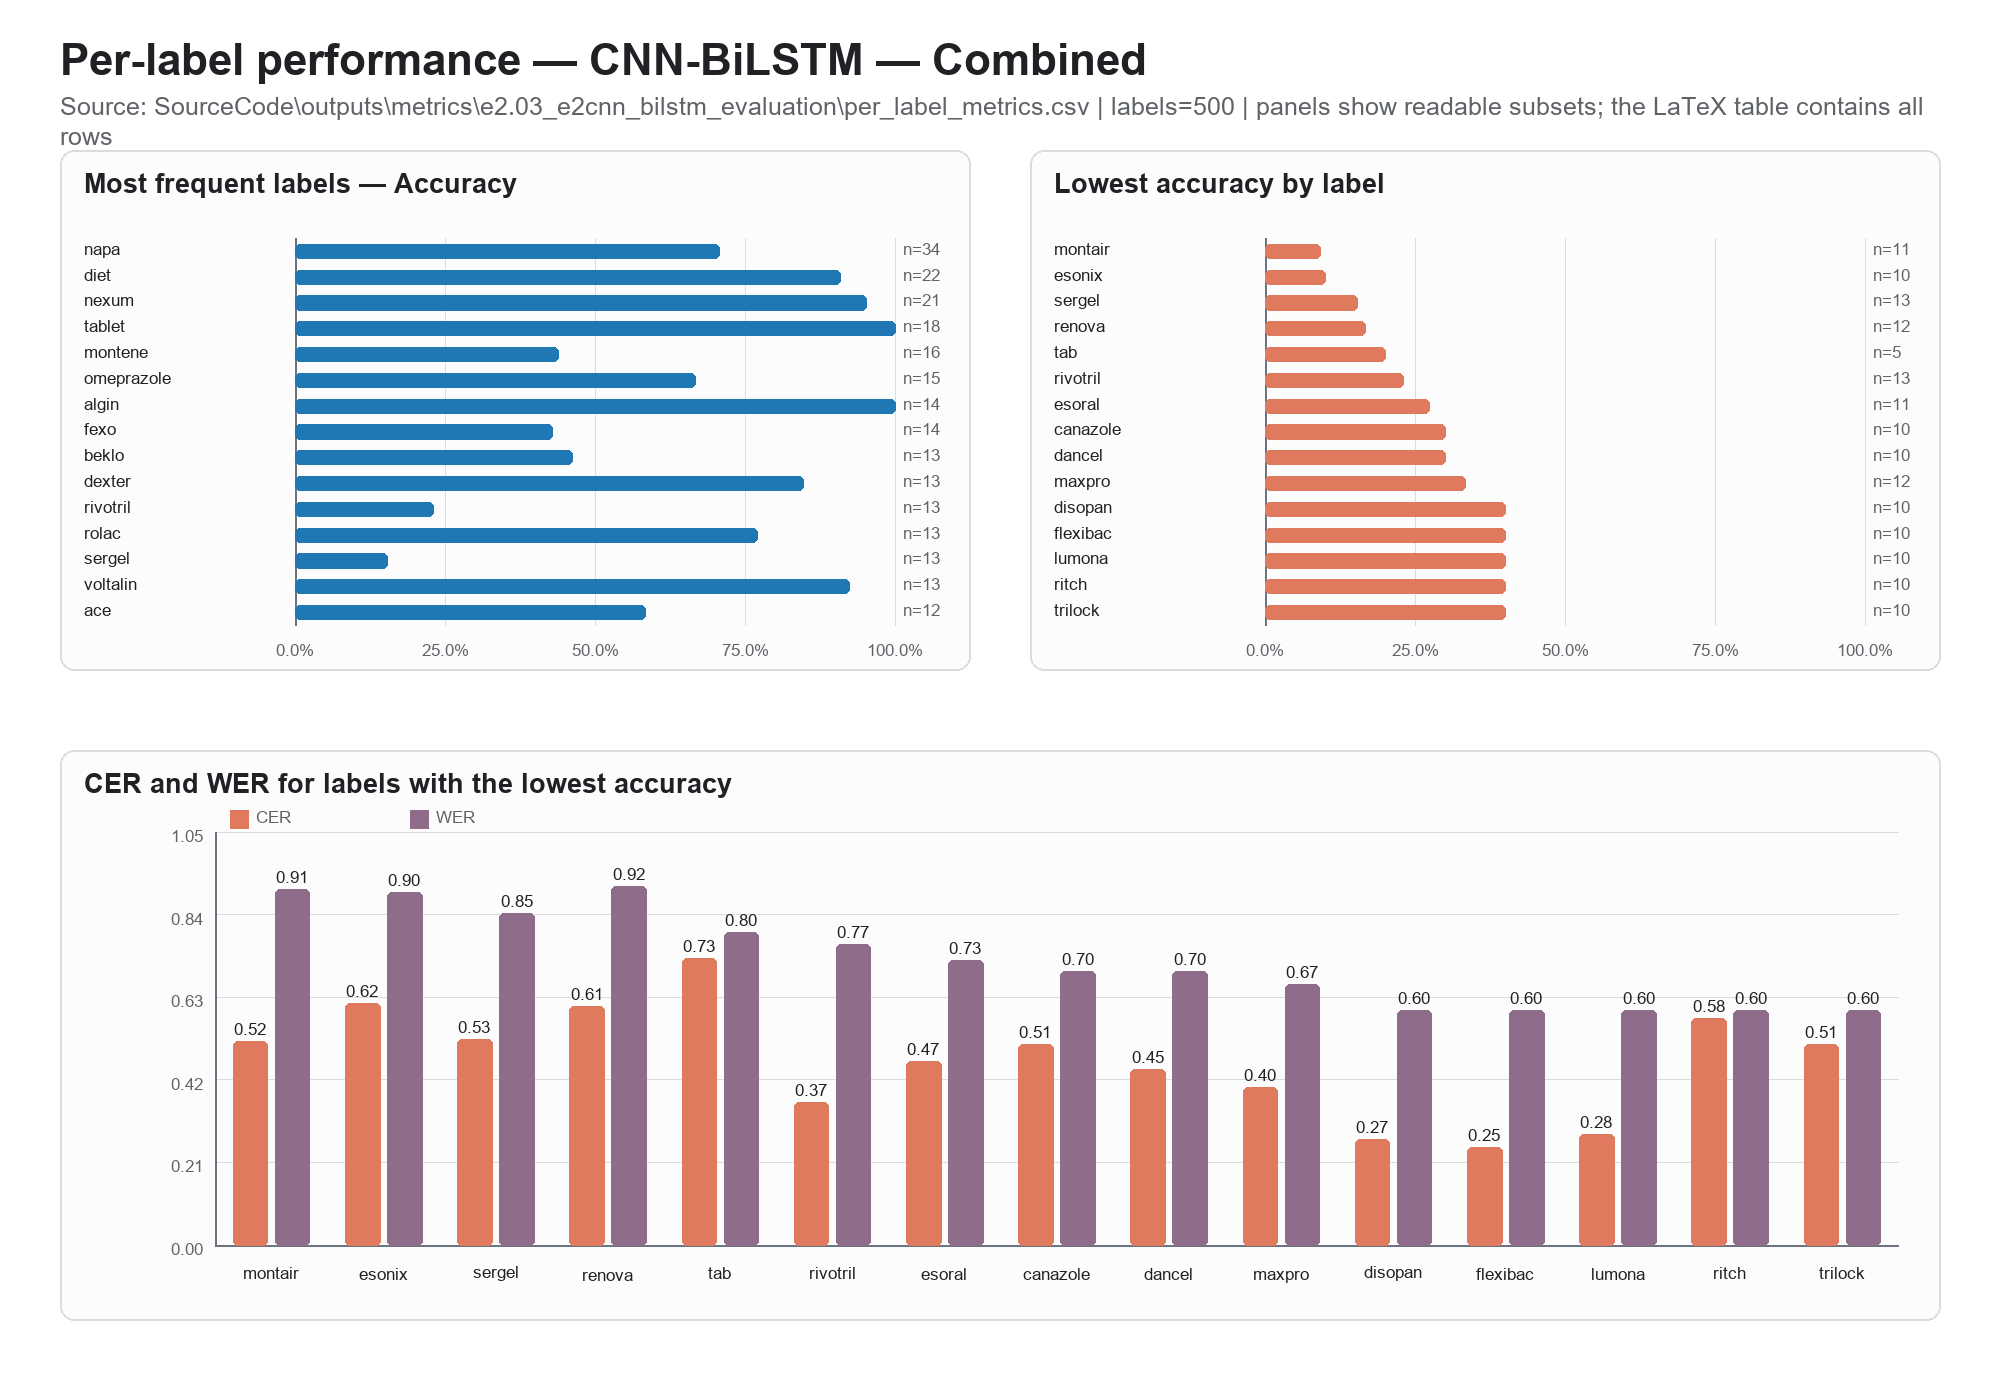
\includegraphics[width=\linewidth]{imagens/evaluation_graficos_tabelas/e2.03_e2cnn_bilstm_evaluation_per_label_metrics.png}
    \caption{Per-label metrics.}
  \end{subfigure}
  \caption{CNN-BiLSTM evaluated in the combined scenario.}
  \label{fig:diagnostic-e2-combined}
\end{figure}

\subsubsection{TrOCR}

\begin{figure}[H]
  \centering
  \begin{subfigure}{0.49\linewidth}
    \centering
    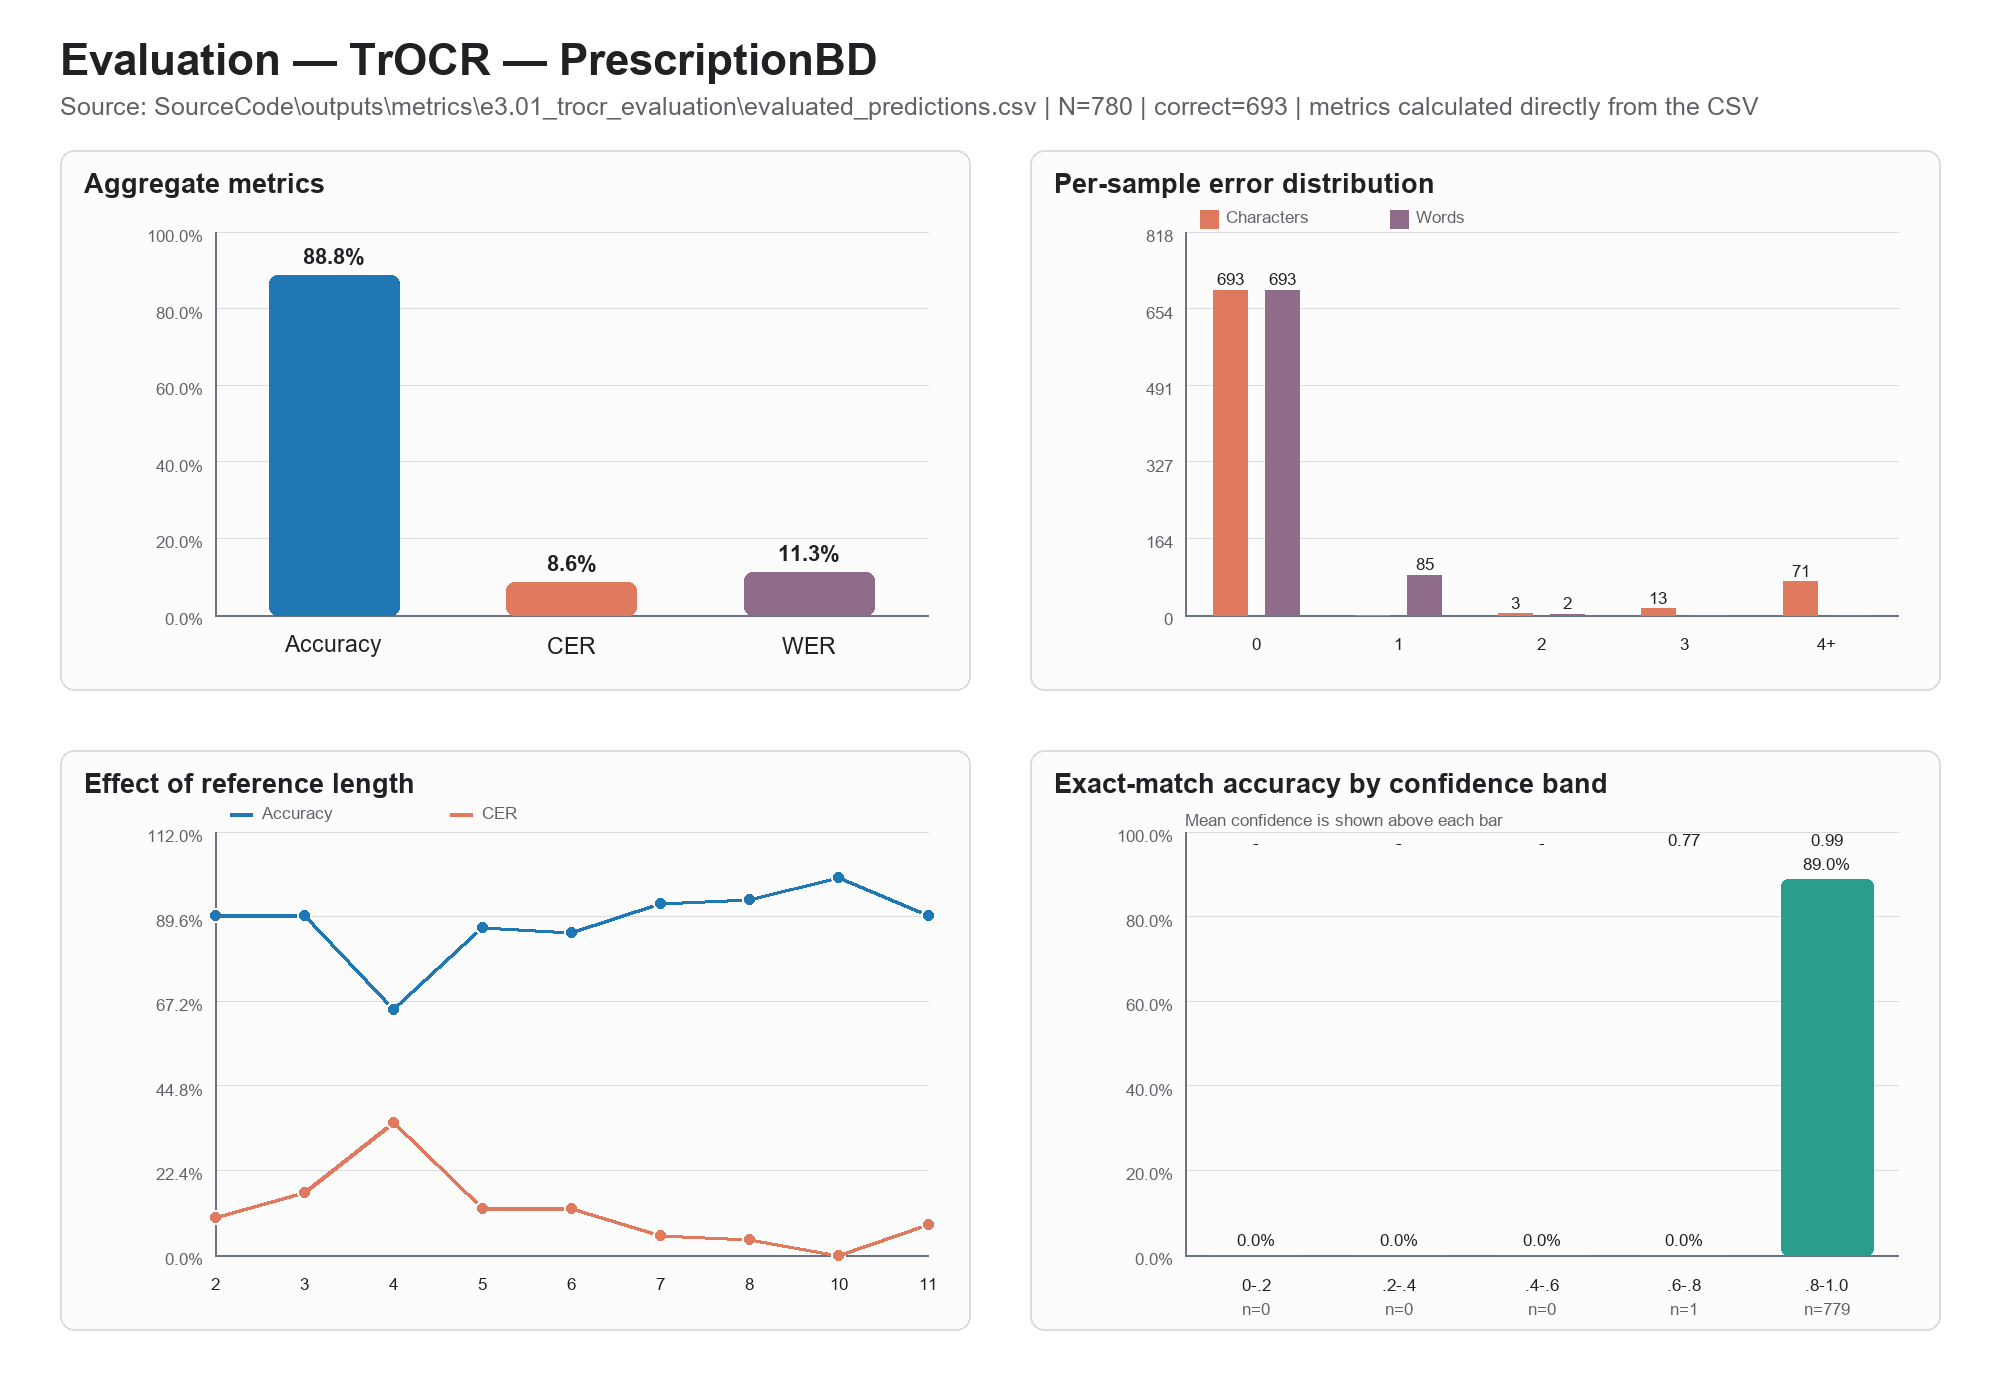
\includegraphics[width=\linewidth]{imagens/evaluation_graficos_tabelas/e3.01_trocr_evaluation_evaluated_predictions.png}
    \caption{Evaluated predictions.}
  \end{subfigure}\hfill
  \begin{subfigure}{0.49\linewidth}
    \centering
    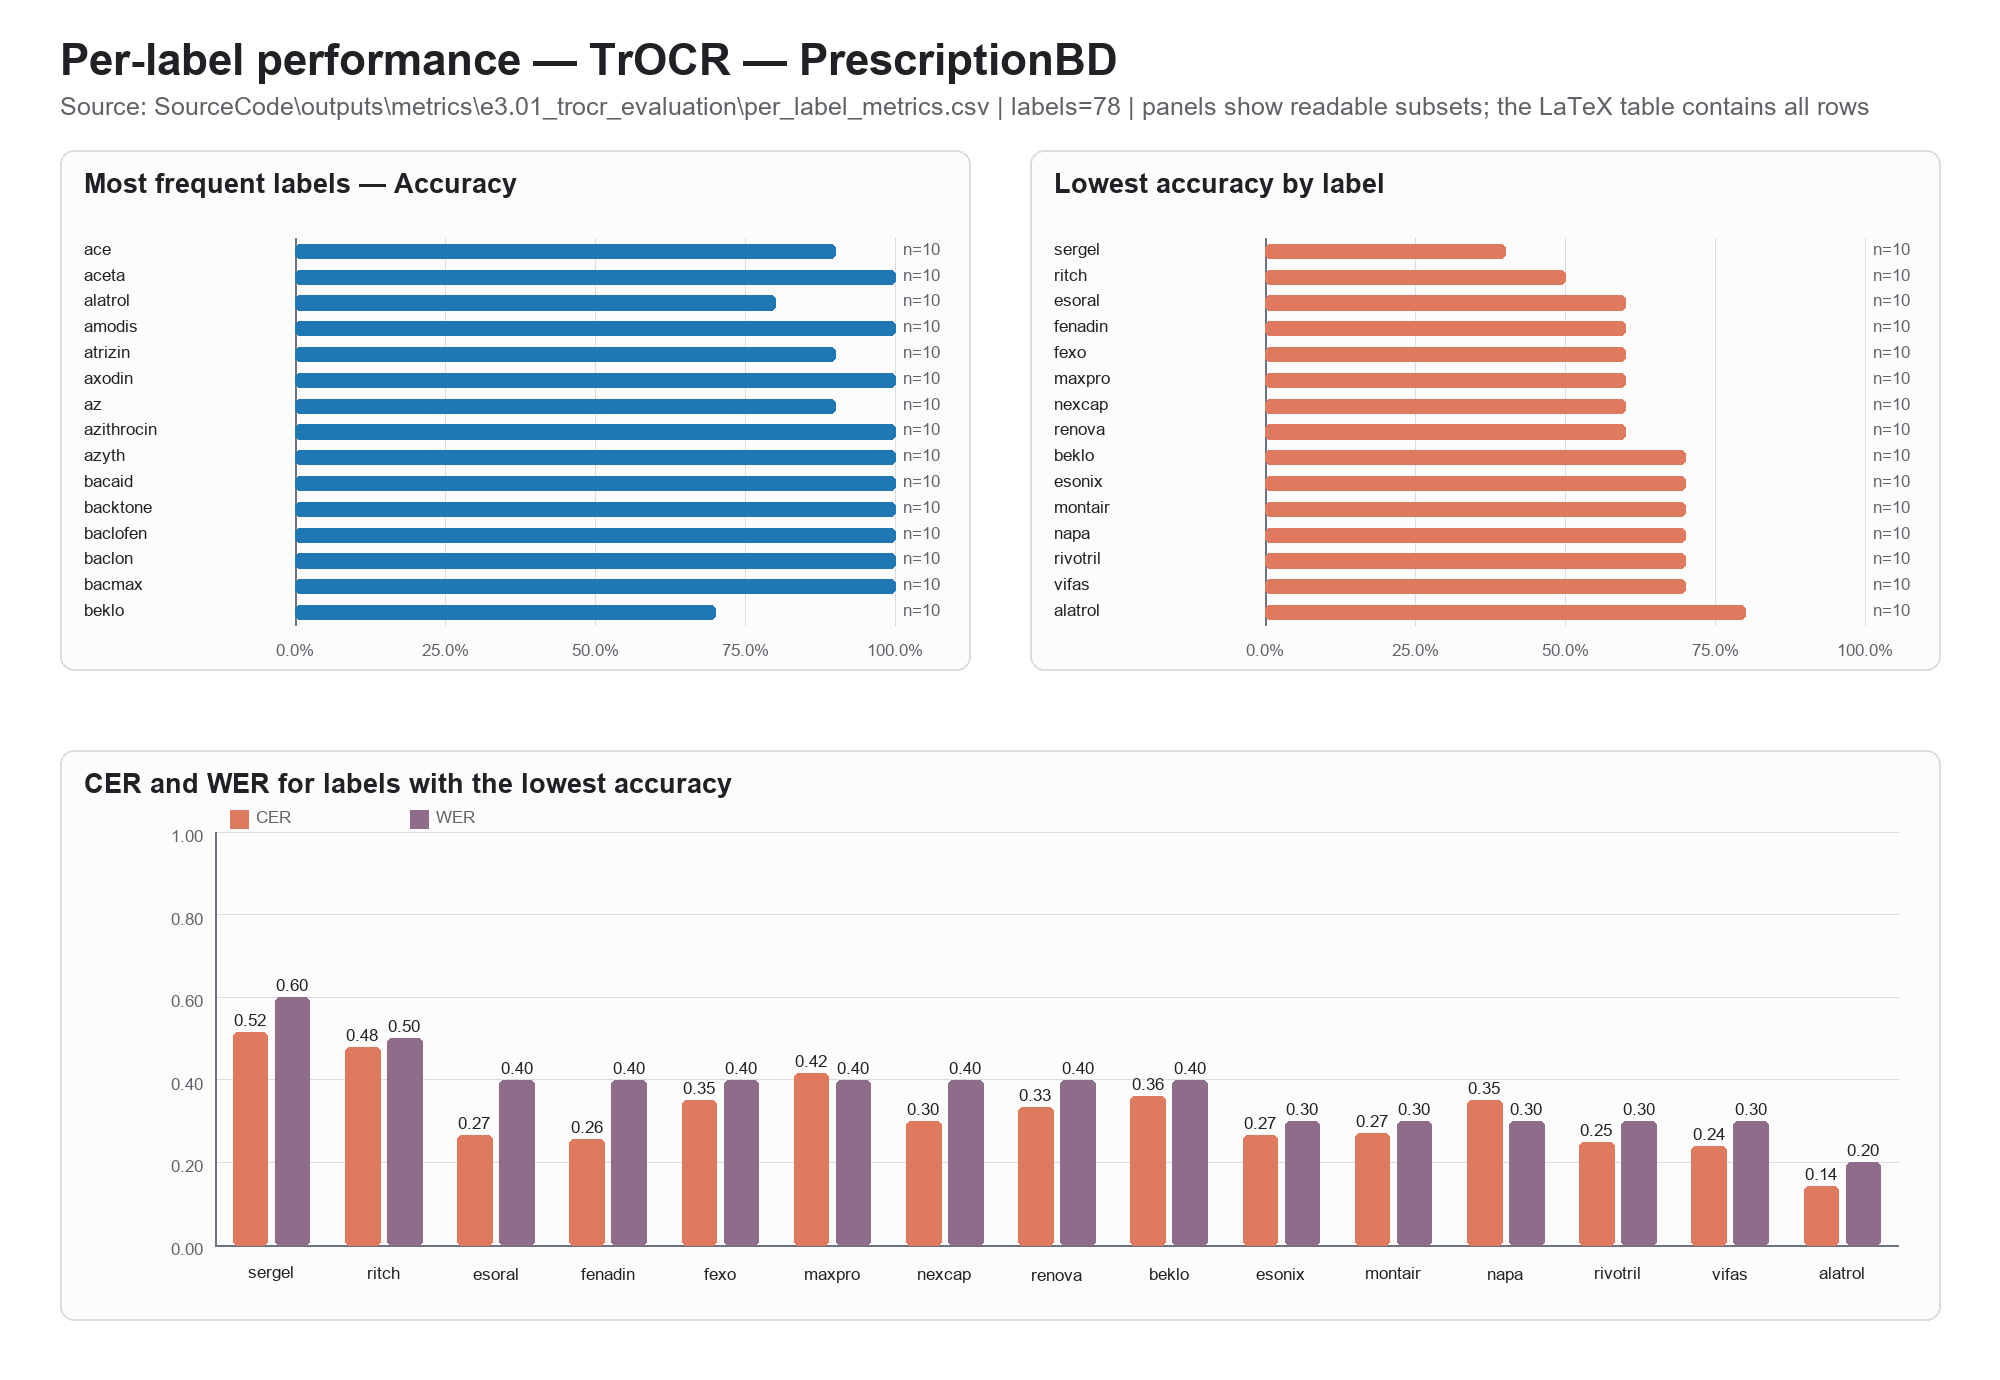
\includegraphics[width=\linewidth]{imagens/evaluation_graficos_tabelas/e3.01_trocr_evaluation_per_label_metrics.png}
    \caption{Per-label metrics.}
  \end{subfigure}
  \caption{TrOCR evaluated on PrescriptionBD.}
  \label{fig:diagnostic-e3-prescriptionbd}
\end{figure}

\begin{figure}[H]
  \centering
  \begin{subfigure}{0.49\linewidth}
    \centering
    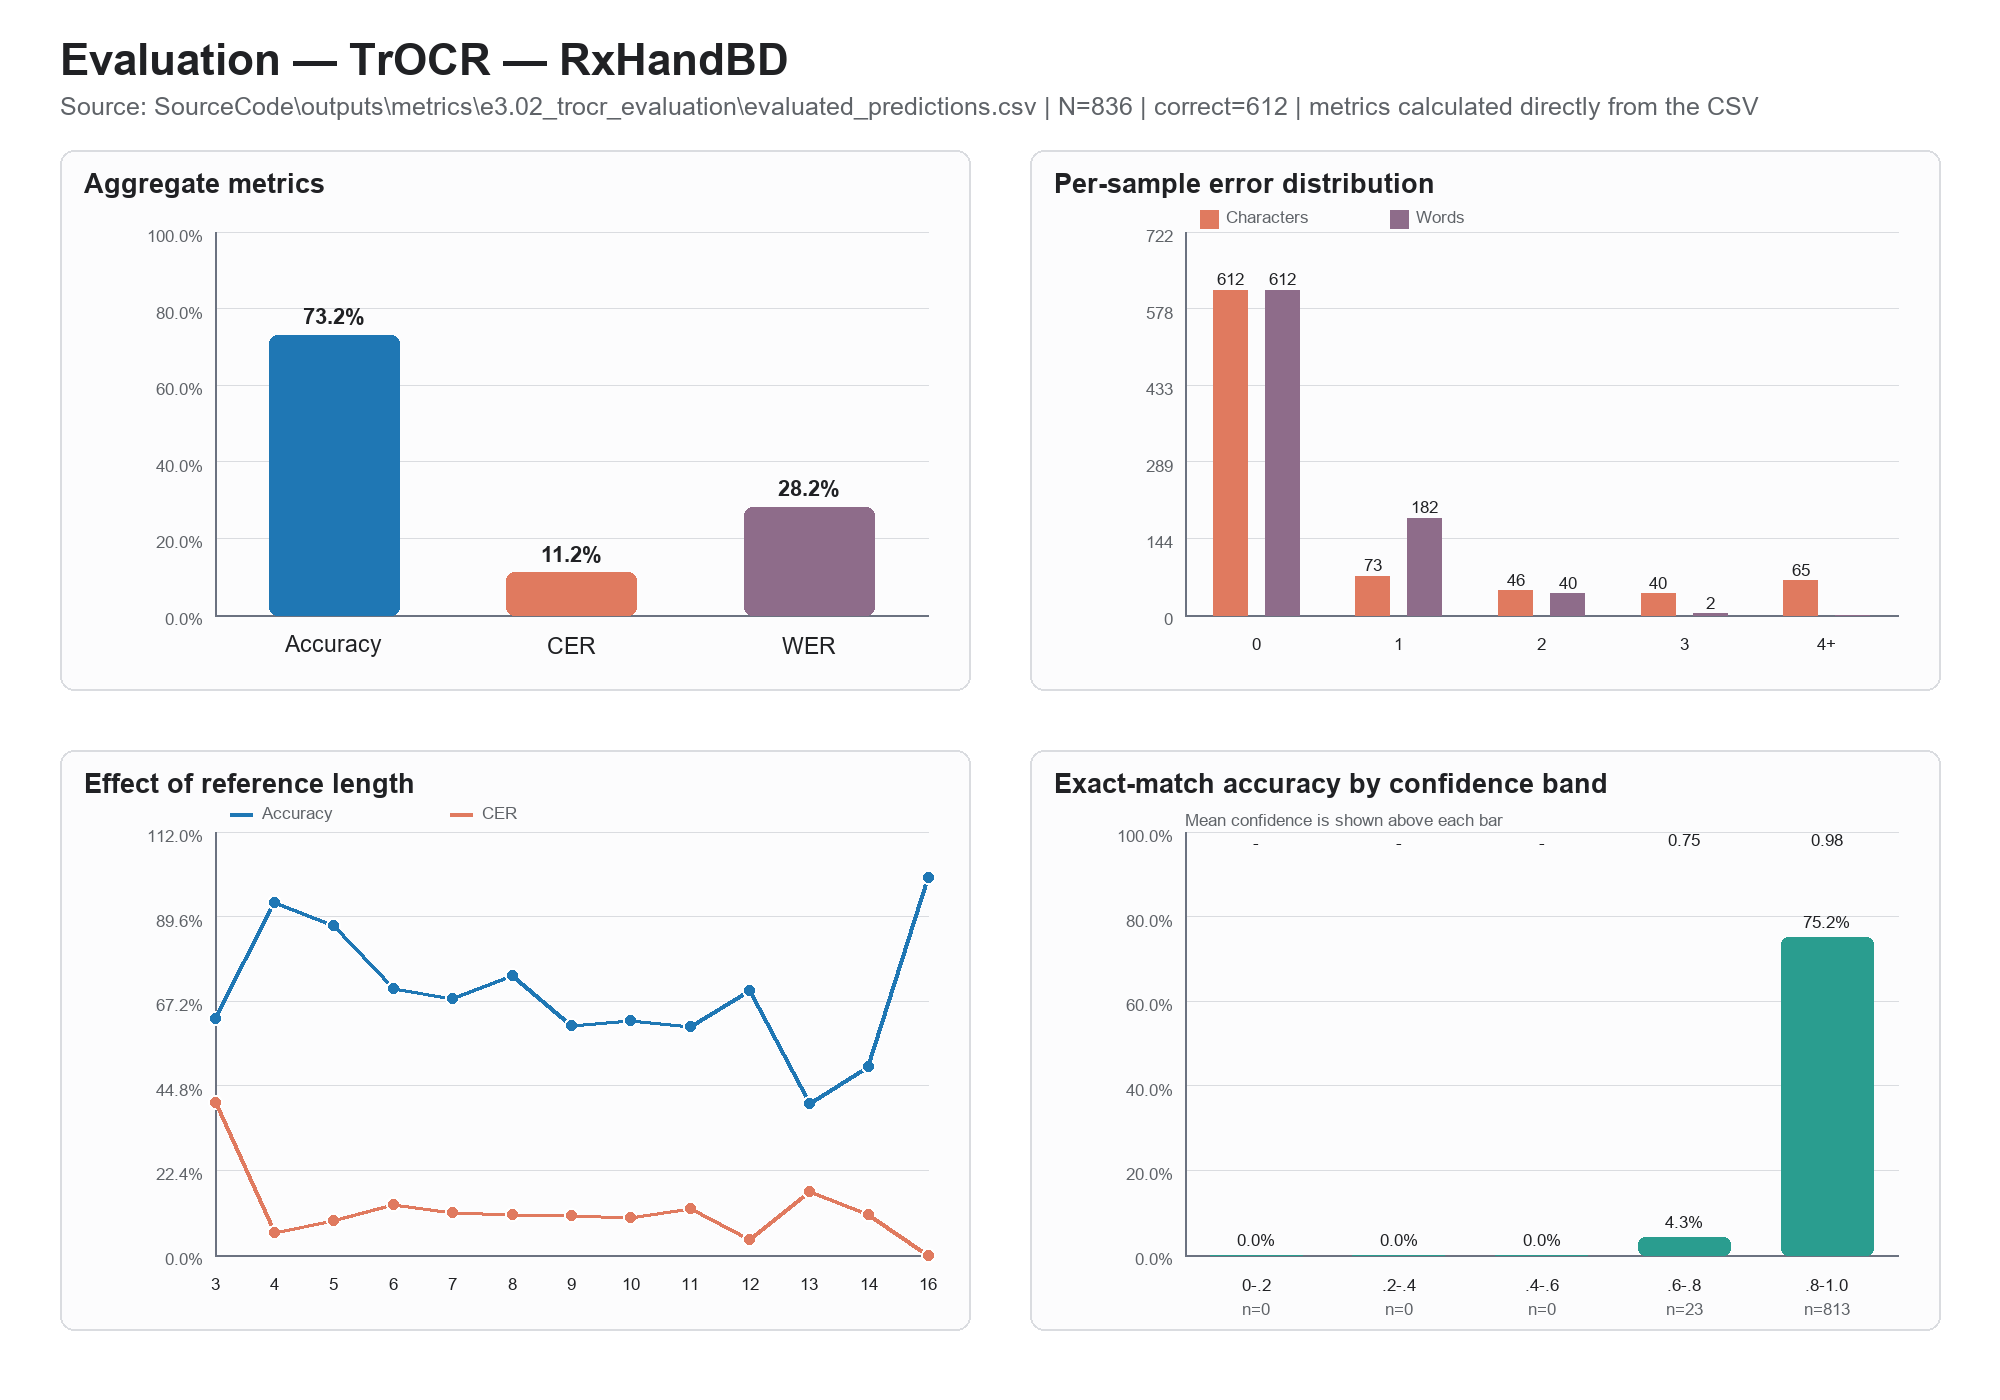
\includegraphics[width=\linewidth]{imagens/evaluation_graficos_tabelas/e3.02_trocr_evaluation_evaluated_predictions.png}
    \caption{Evaluated predictions.}
  \end{subfigure}\hfill
  \begin{subfigure}{0.49\linewidth}
    \centering
    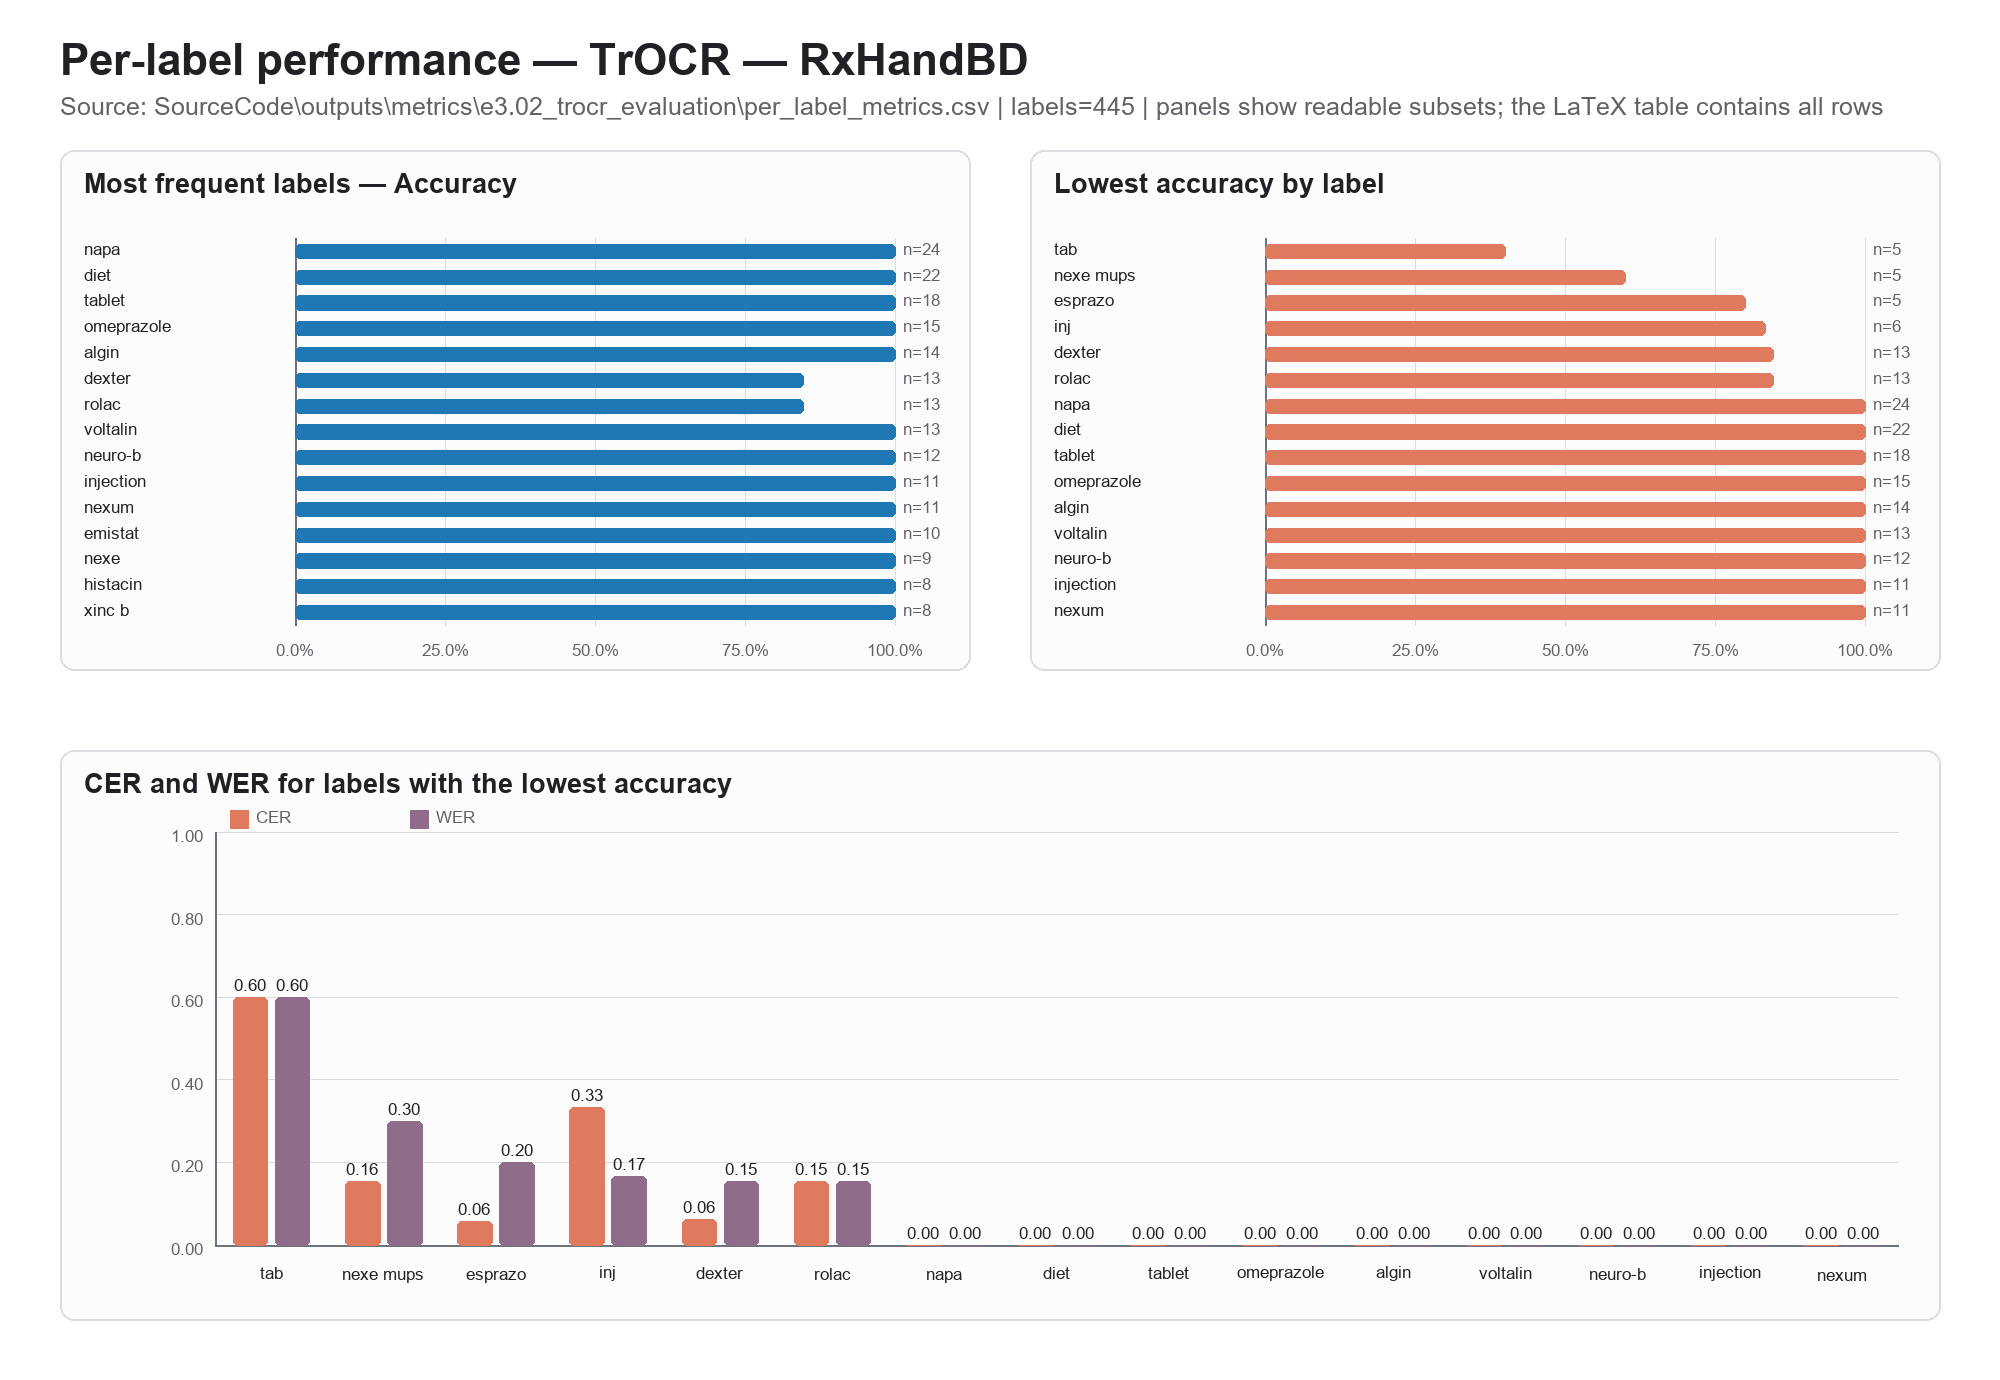
\includegraphics[width=\linewidth]{imagens/evaluation_graficos_tabelas/e3.02_trocr_evaluation_per_label_metrics.png}
    \caption{Per-label metrics.}
  \end{subfigure}
  \caption{TrOCR evaluated on RxHandBD.}
  \label{fig:diagnostic-e3-rxhandbd}
\end{figure}

\begin{figure}[H]
  \centering
  \begin{subfigure}{0.49\linewidth}
    \centering
    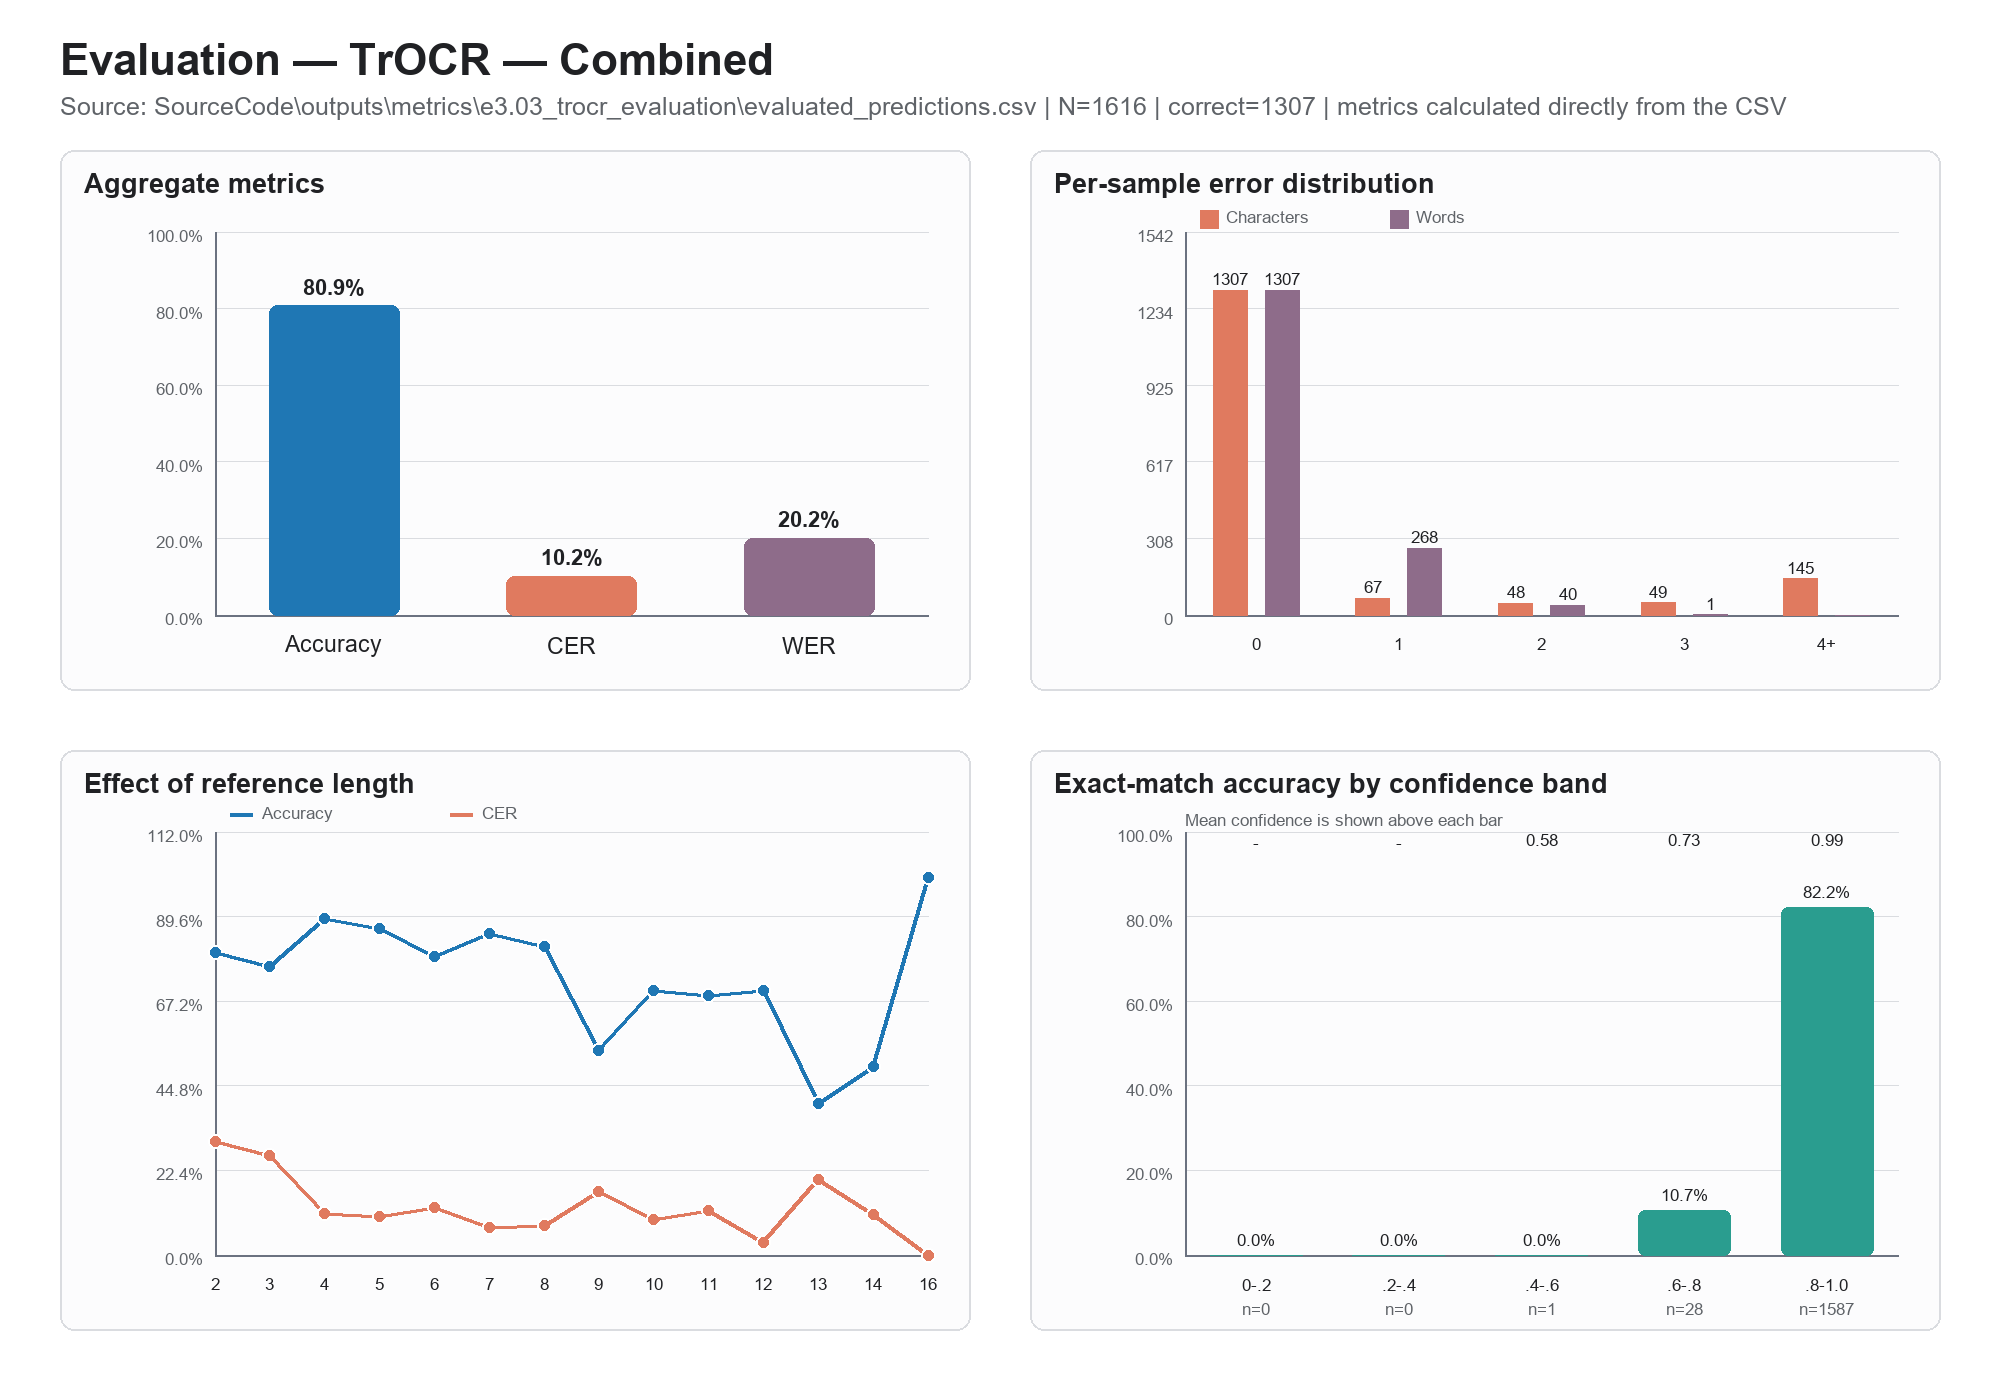
\includegraphics[width=\linewidth]{imagens/evaluation_graficos_tabelas/e3.03_trocr_evaluation_evaluated_predictions.png}
    \caption{Evaluated predictions.}
  \end{subfigure}\hfill
  \begin{subfigure}{0.49\linewidth}
    \centering
    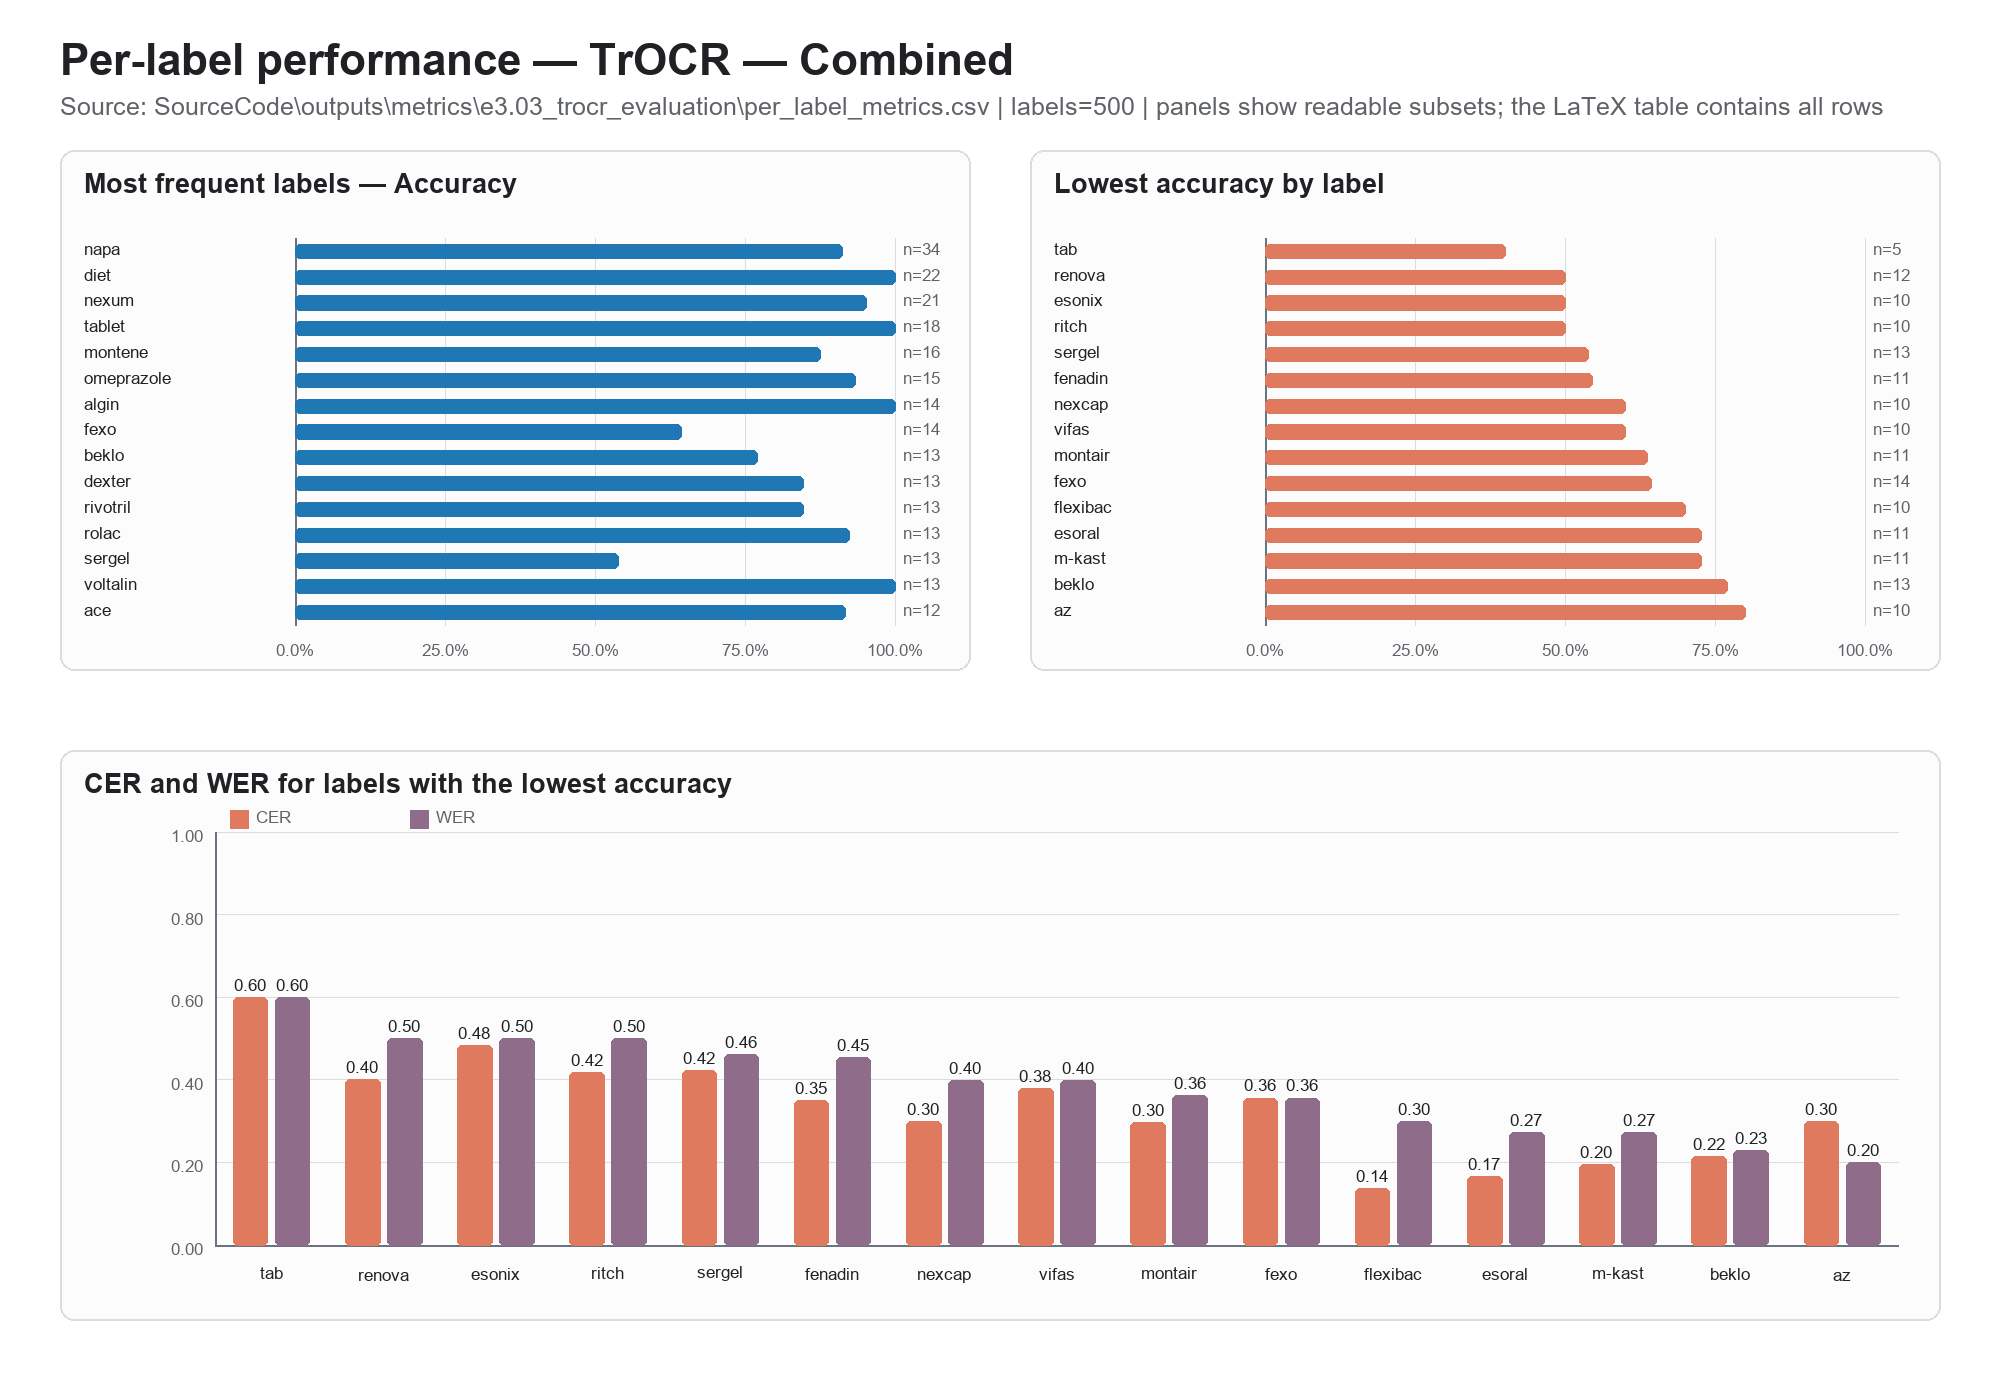
\includegraphics[width=\linewidth]{imagens/evaluation_graficos_tabelas/e3.03_trocr_evaluation_per_label_metrics.png}
    \caption{Per-label metrics.}
  \end{subfigure}
  \caption{TrOCR evaluated in the combined scenario.}
  \label{fig:diagnostic-e3-combined}
\end{figure}

\subsubsection{PARSeq}

\begin{figure}[H]
  \centering
  \begin{subfigure}{0.49\linewidth}
    \centering
    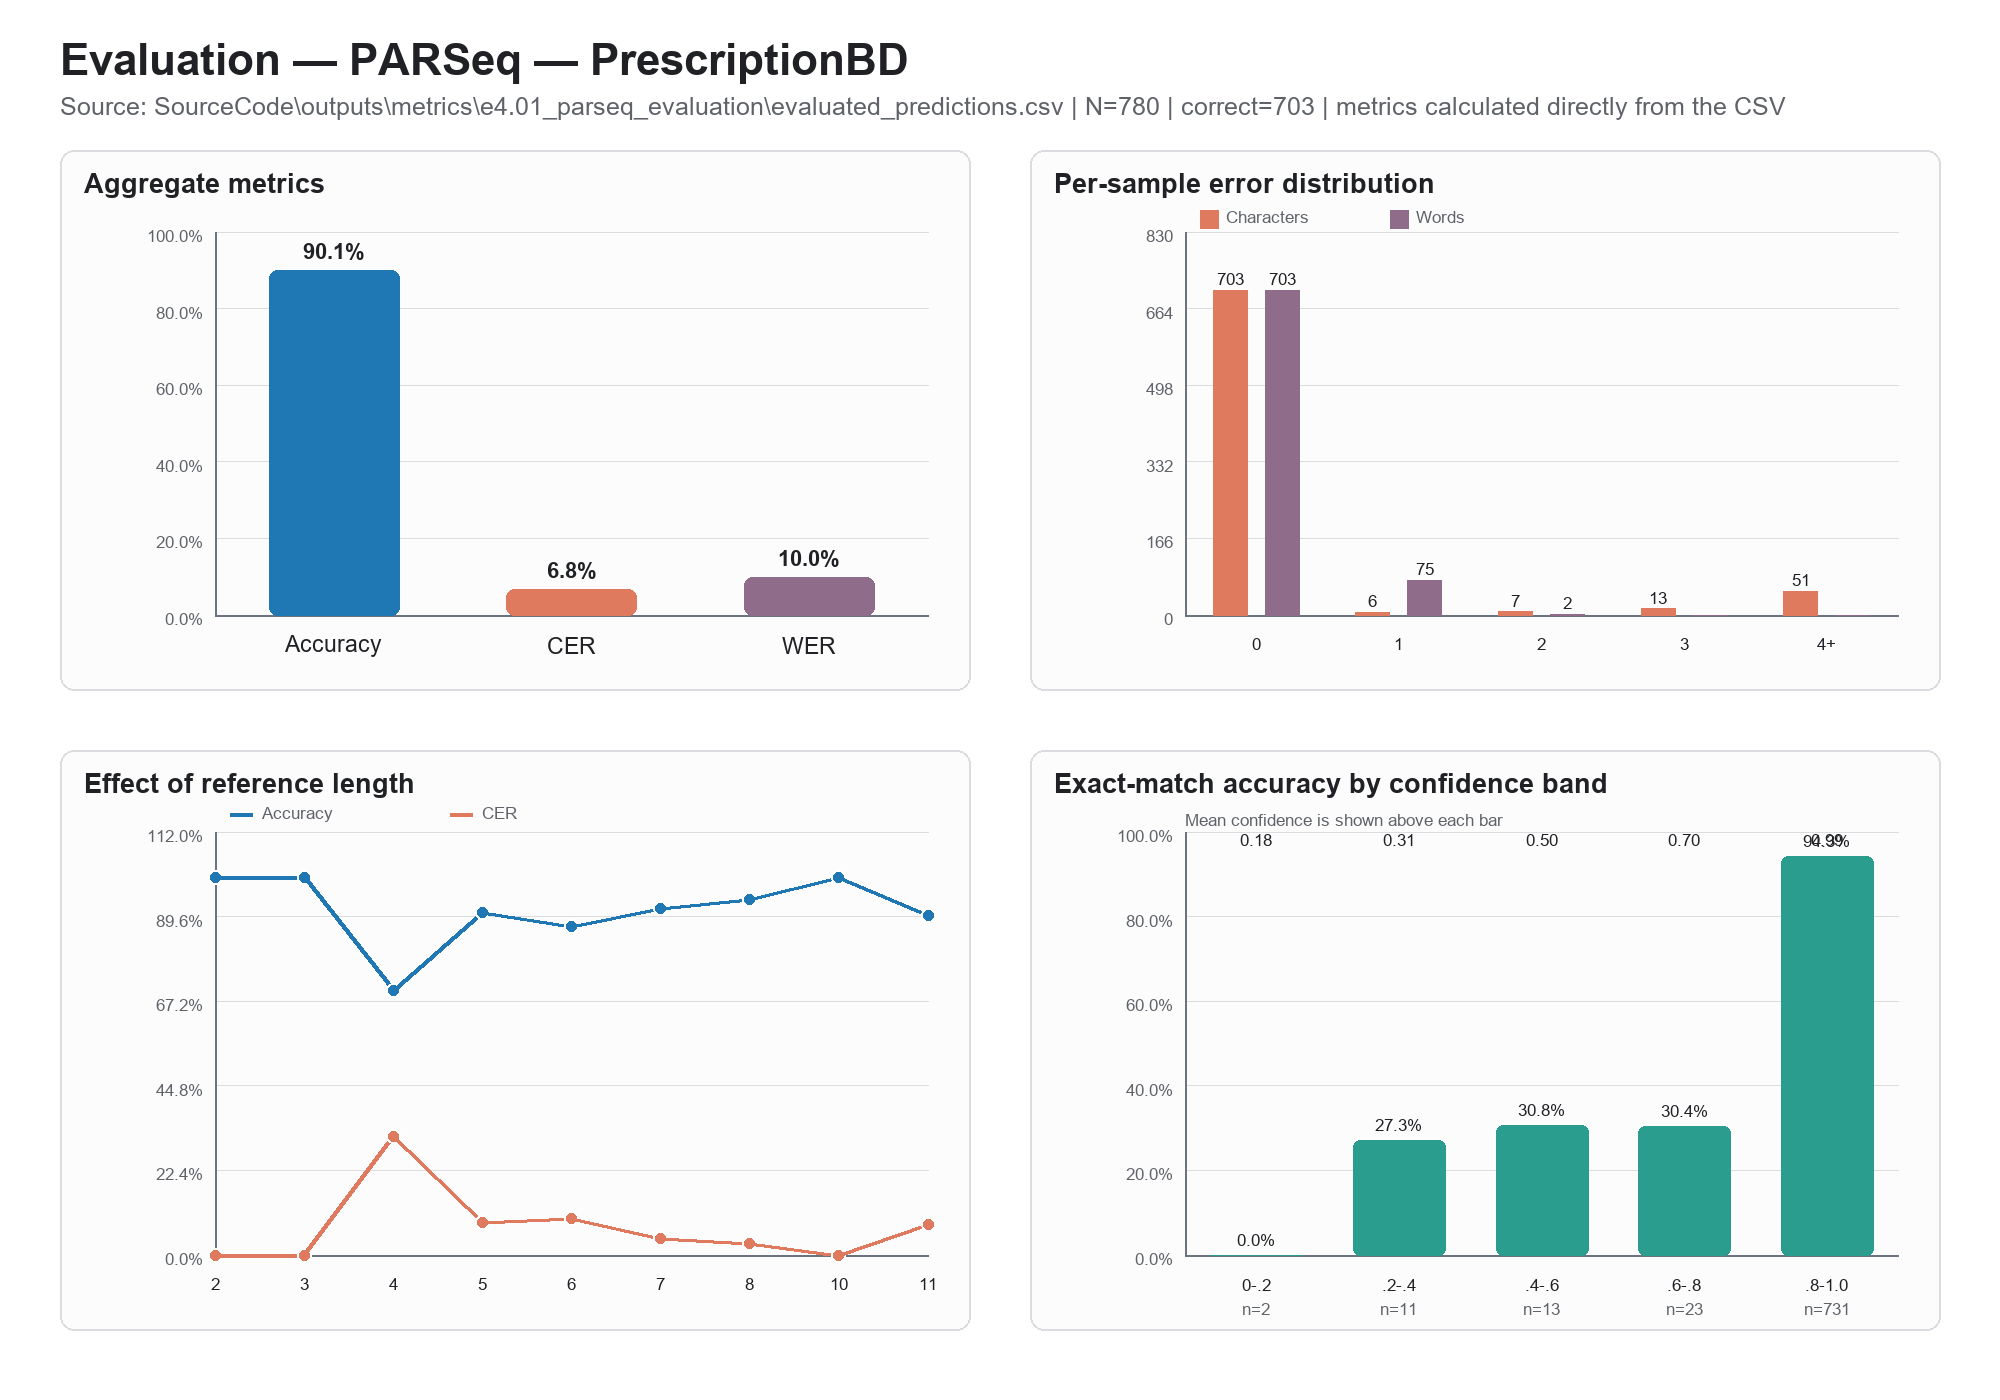
\includegraphics[width=\linewidth]{imagens/evaluation_graficos_tabelas/e4.01_parseq_evaluation_evaluated_predictions.png}
    \caption{Evaluated predictions.}
  \end{subfigure}\hfill
  \begin{subfigure}{0.49\linewidth}
    \centering
    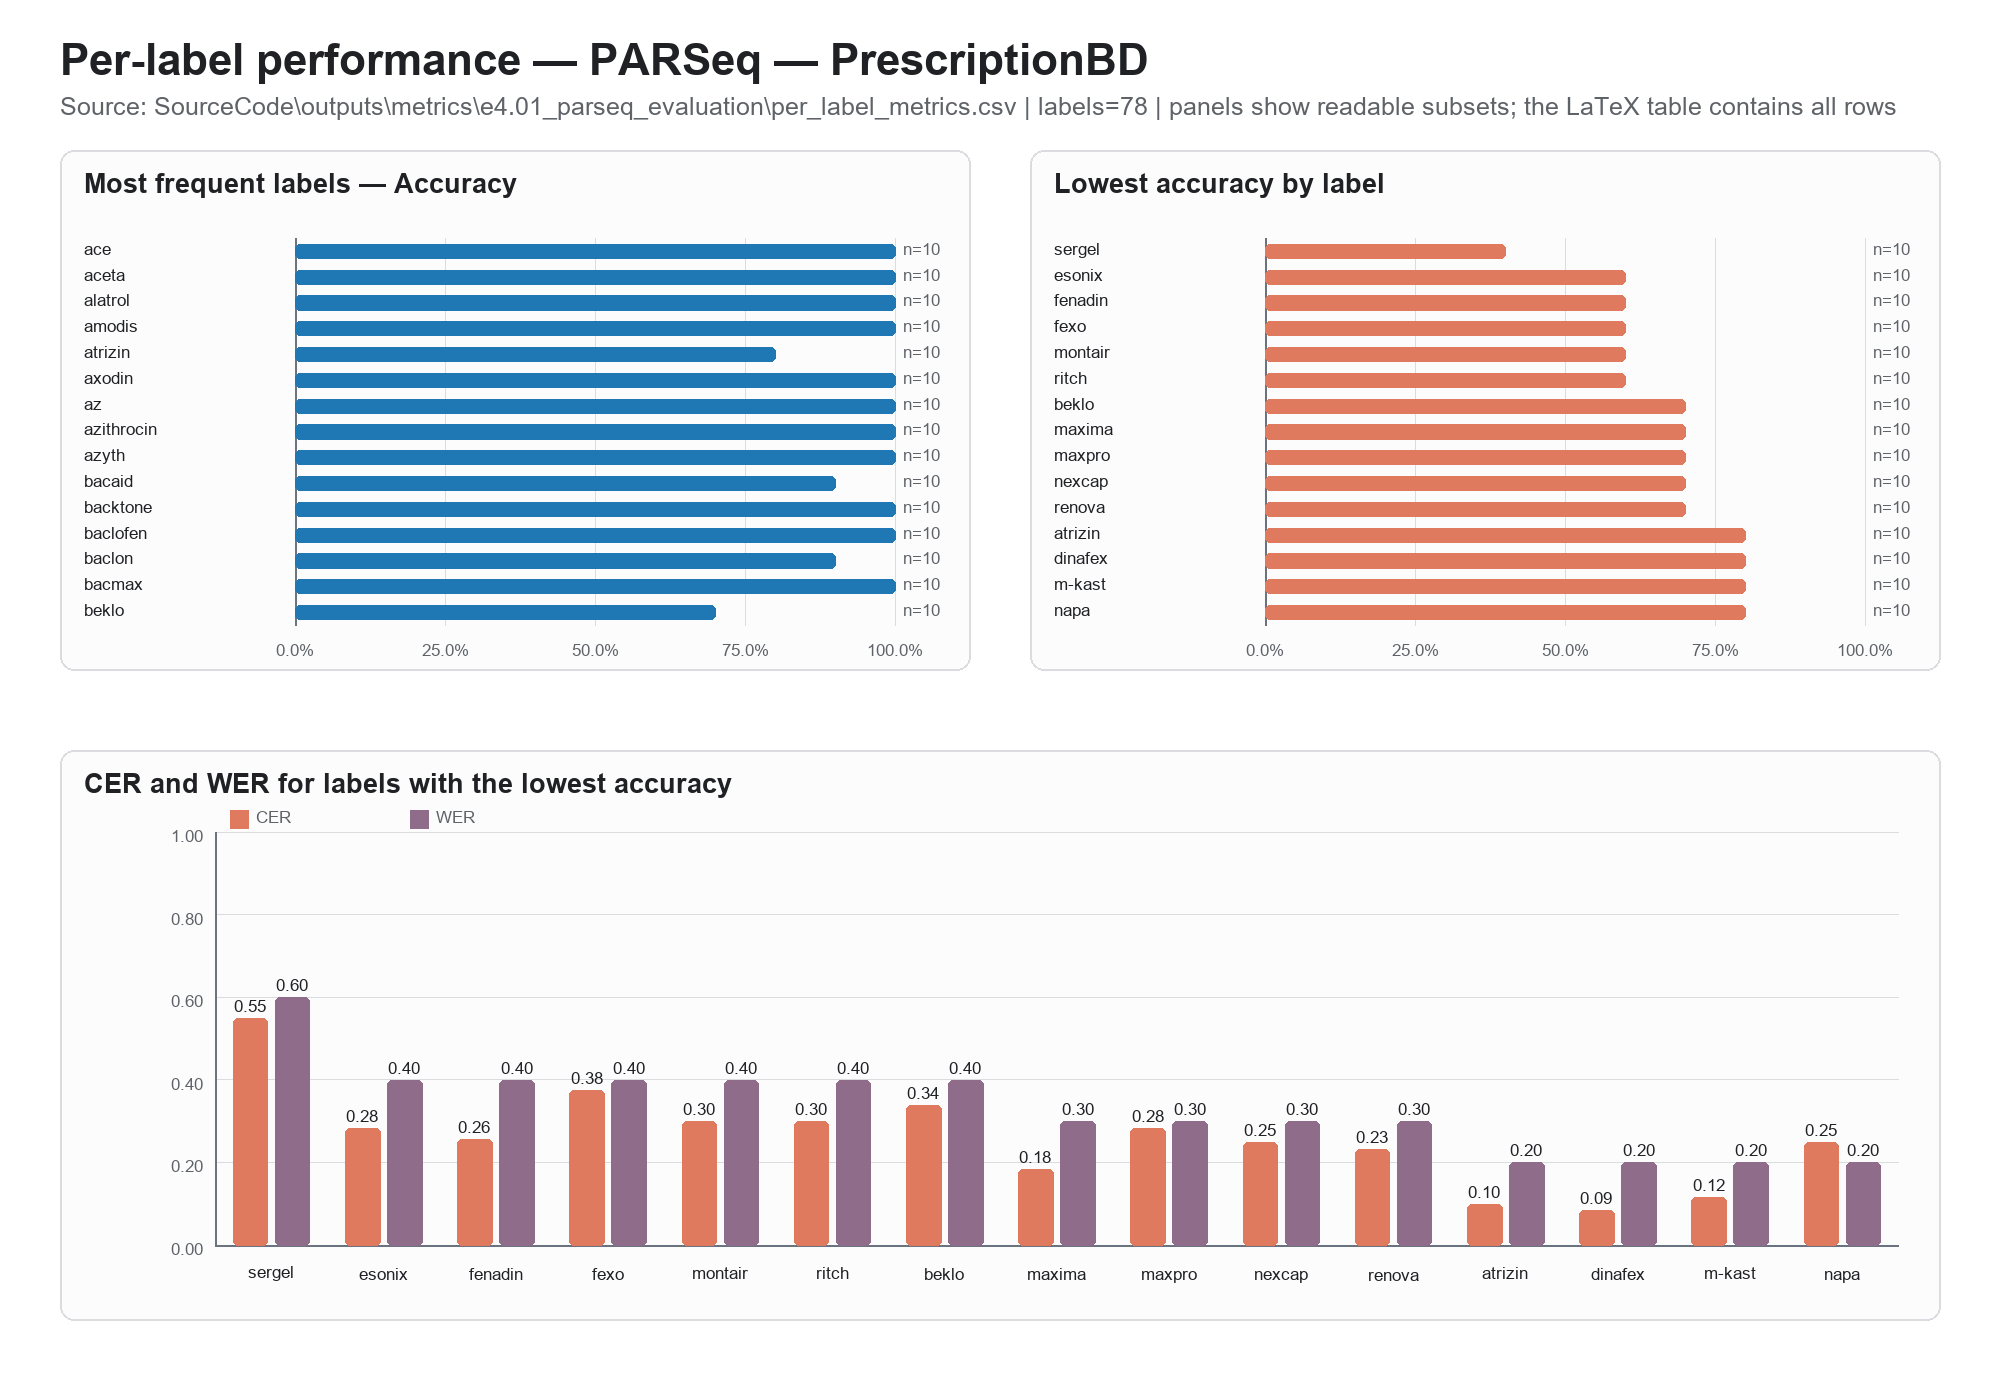
\includegraphics[width=\linewidth]{imagens/evaluation_graficos_tabelas/e4.01_parseq_evaluation_per_label_metrics.png}
    \caption{Per-label metrics.}
  \end{subfigure}
  \caption{PARSeq evaluated on PrescriptionBD.}
  \label{fig:diagnostic-e4-prescriptionbd}
\end{figure}

\begin{figure}[H]
  \centering
  \begin{subfigure}{0.49\linewidth}
    \centering
    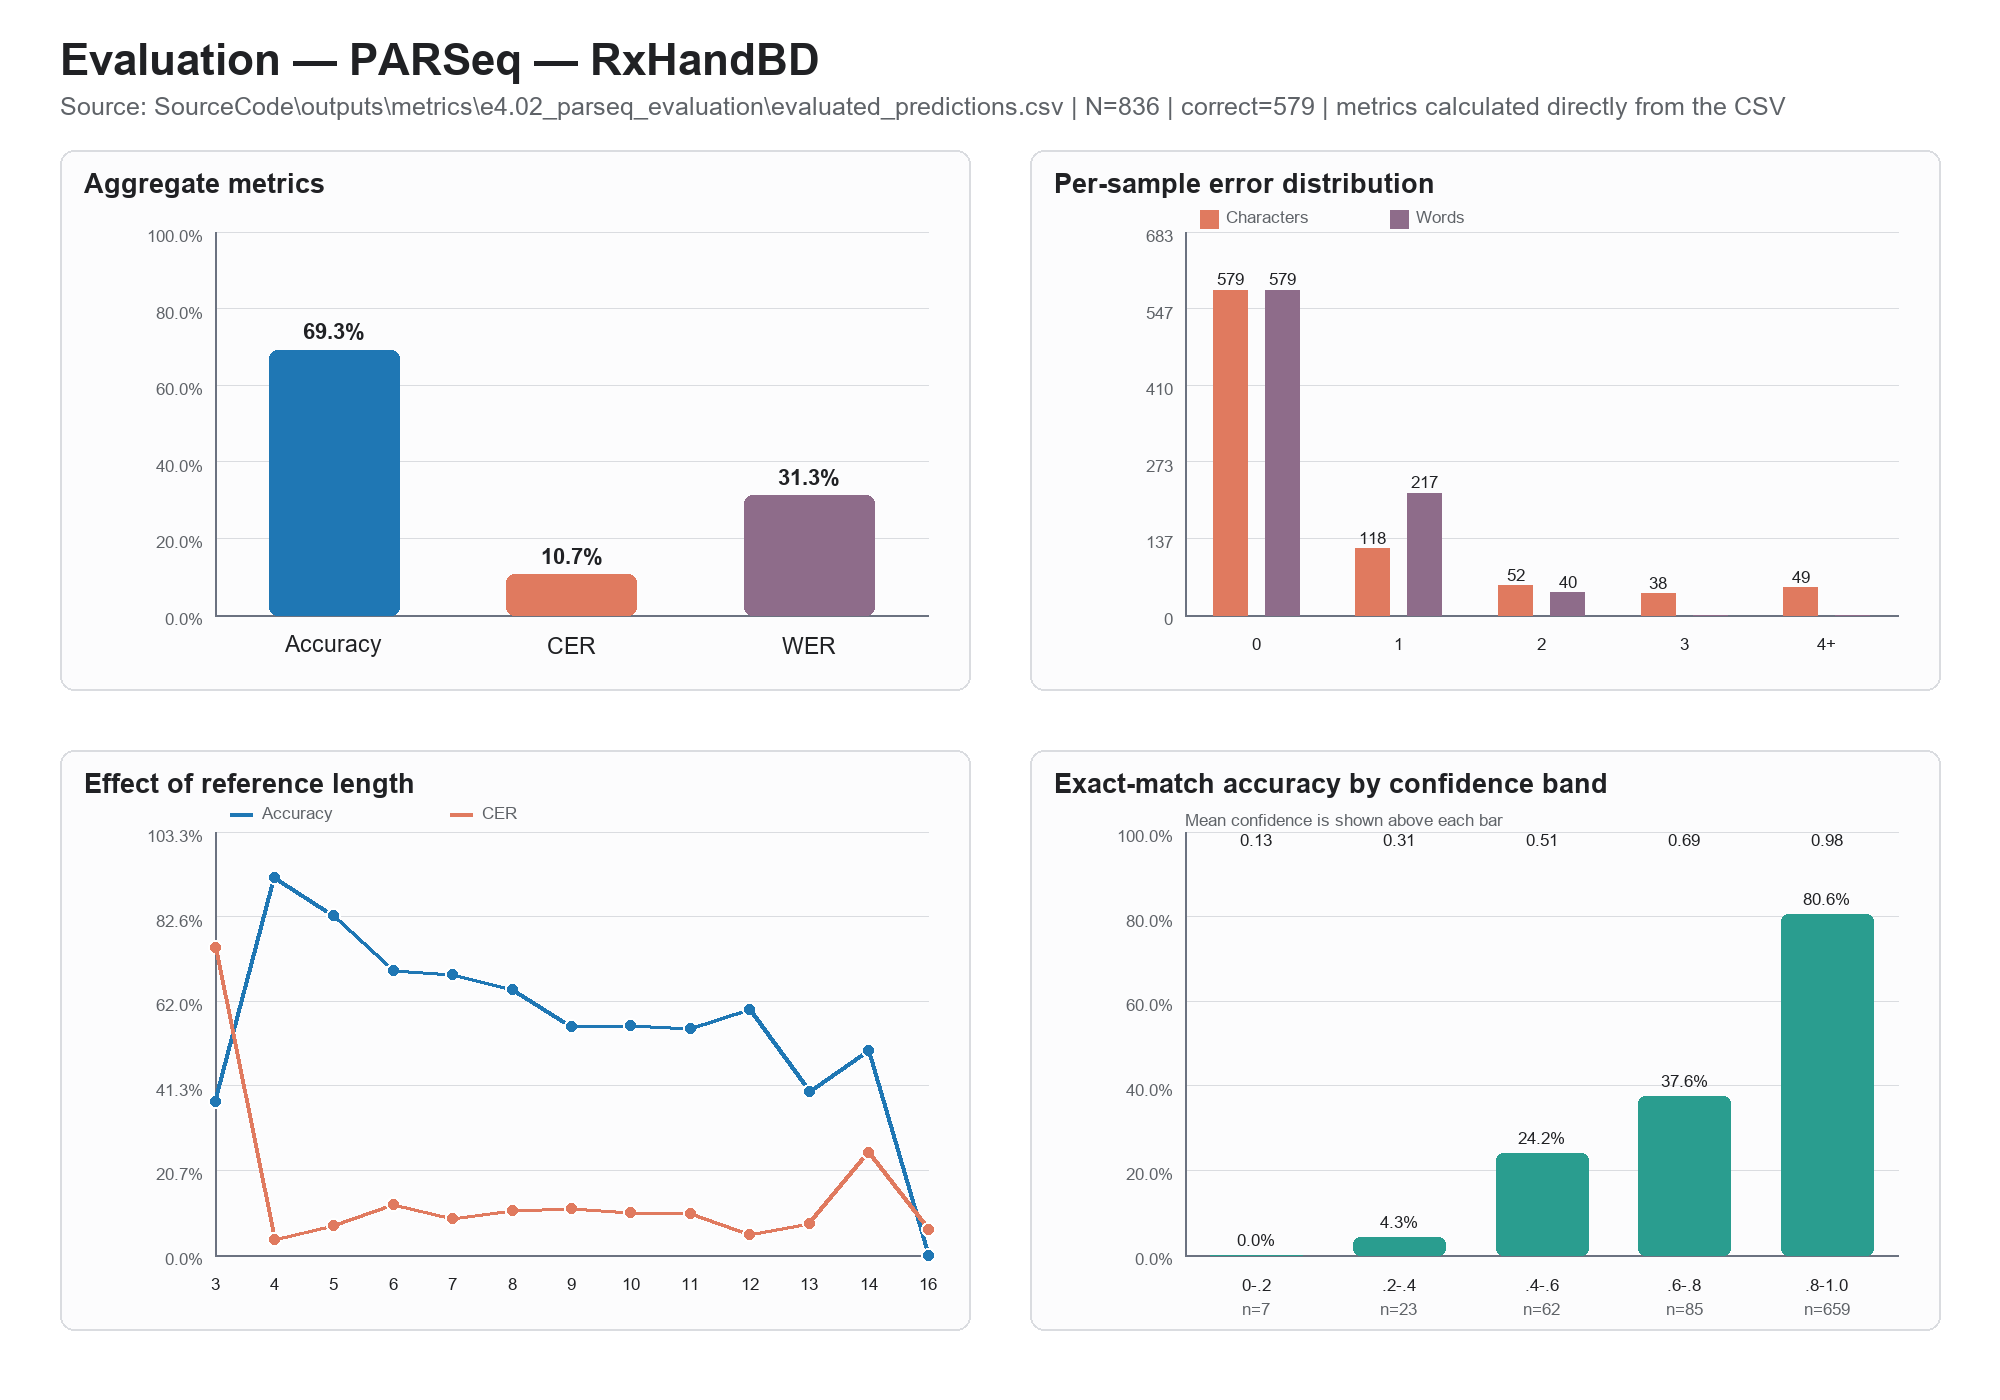
\includegraphics[width=\linewidth]{imagens/evaluation_graficos_tabelas/e4.02_parseq_evaluation_evaluated_predictions.png}
    \caption{Evaluated predictions.}
  \end{subfigure}\hfill
  \begin{subfigure}{0.49\linewidth}
    \centering
    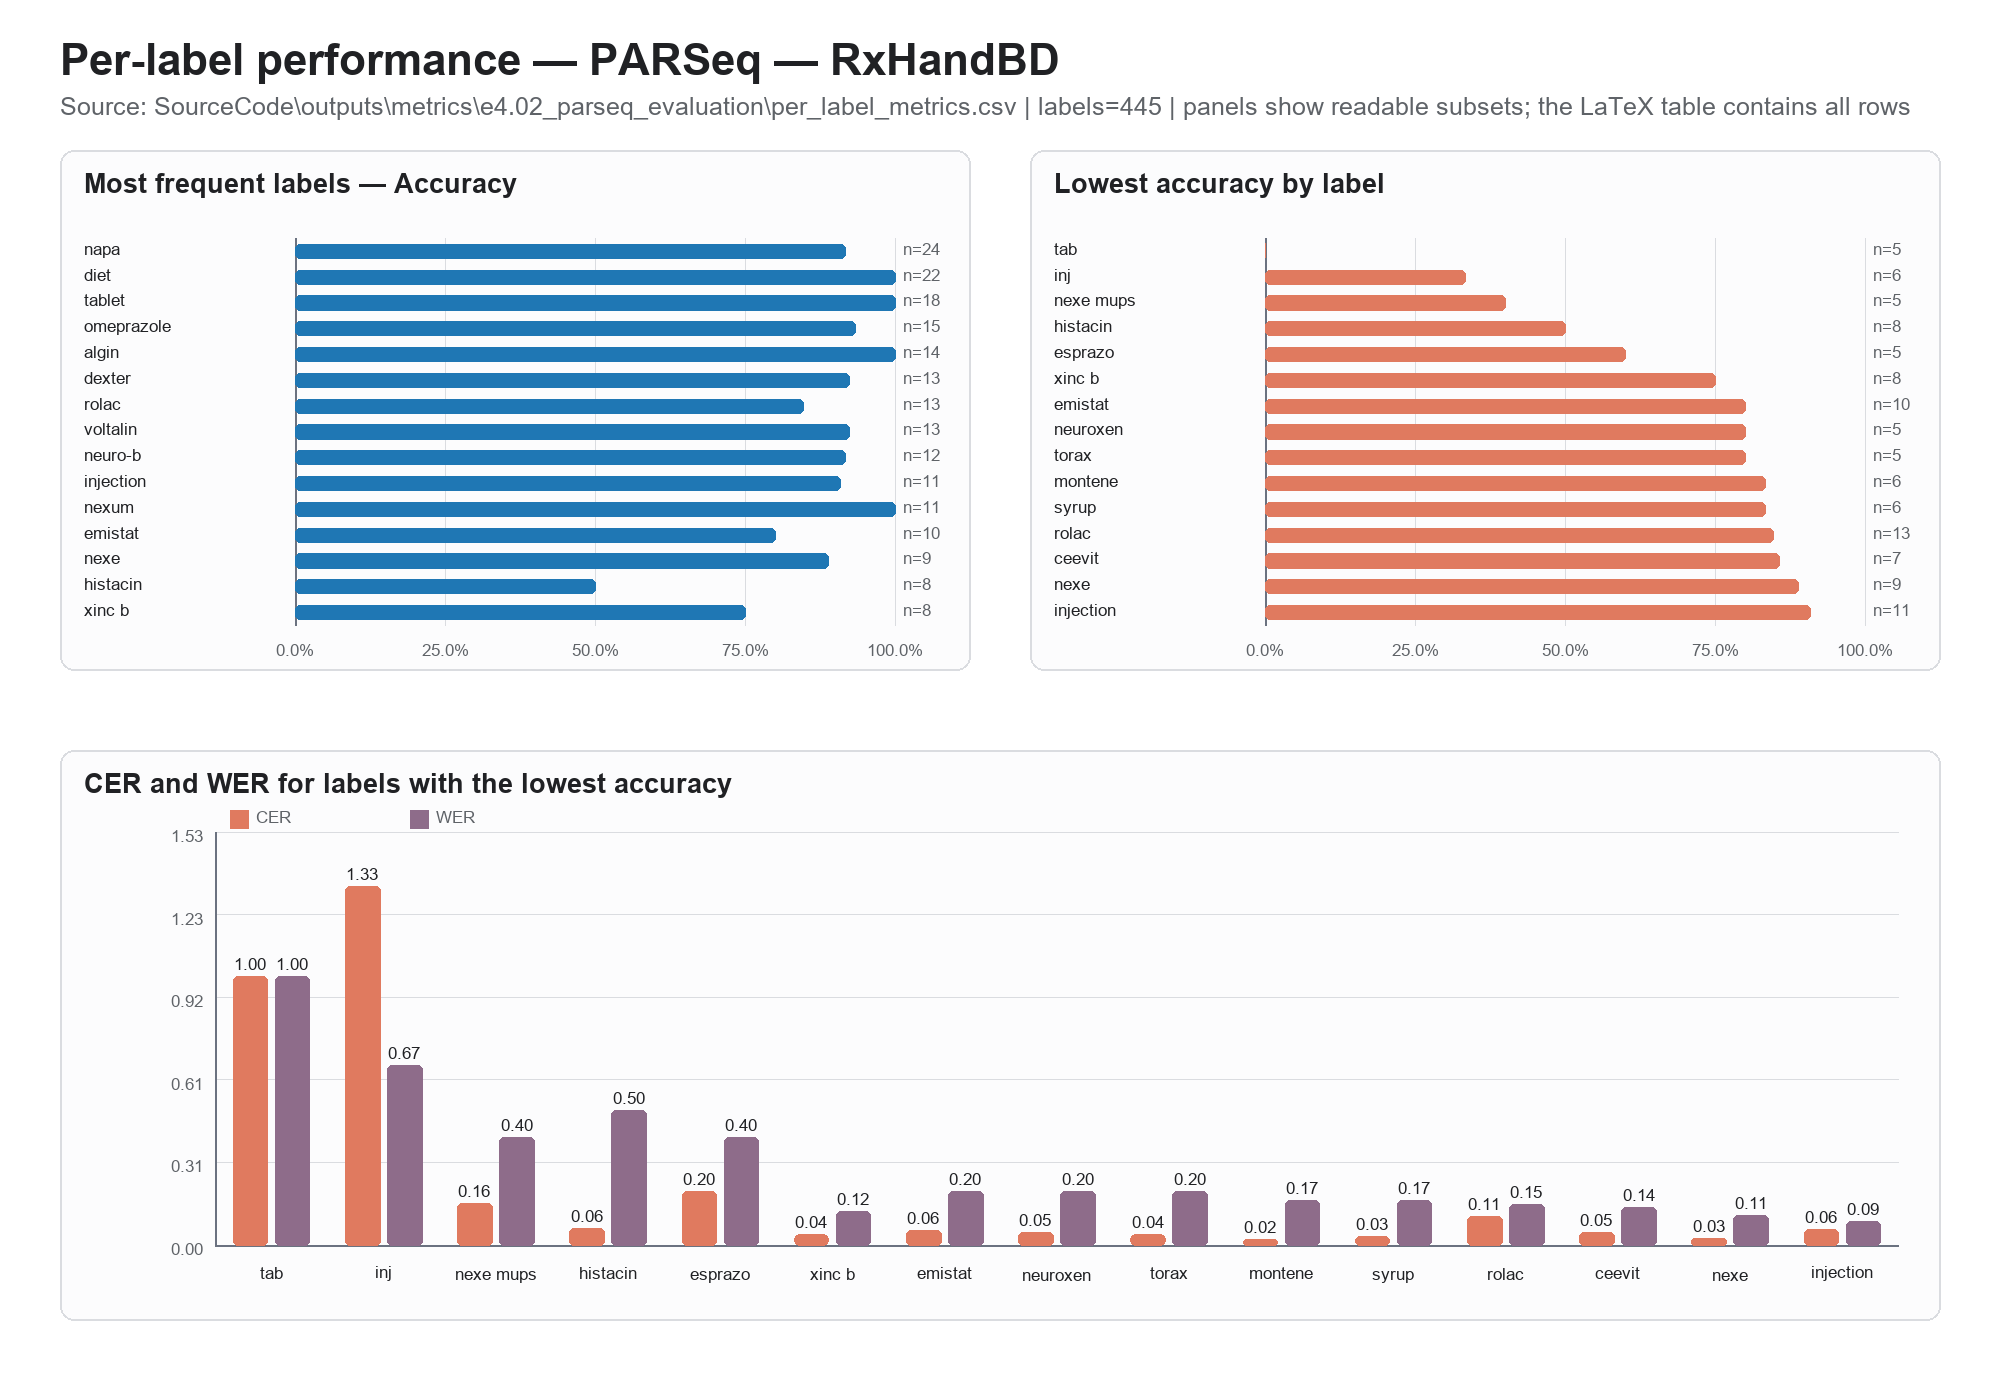
\includegraphics[width=\linewidth]{imagens/evaluation_graficos_tabelas/e4.02_parseq_evaluation_per_label_metrics.png}
    \caption{Per-label metrics.}
  \end{subfigure}
  \caption{PARSeq evaluated on RxHandBD.}
  \label{fig:diagnostic-e4-rxhandbd}
\end{figure}

\begin{figure}[H]
  \centering
  \begin{subfigure}{0.49\linewidth}
    \centering
    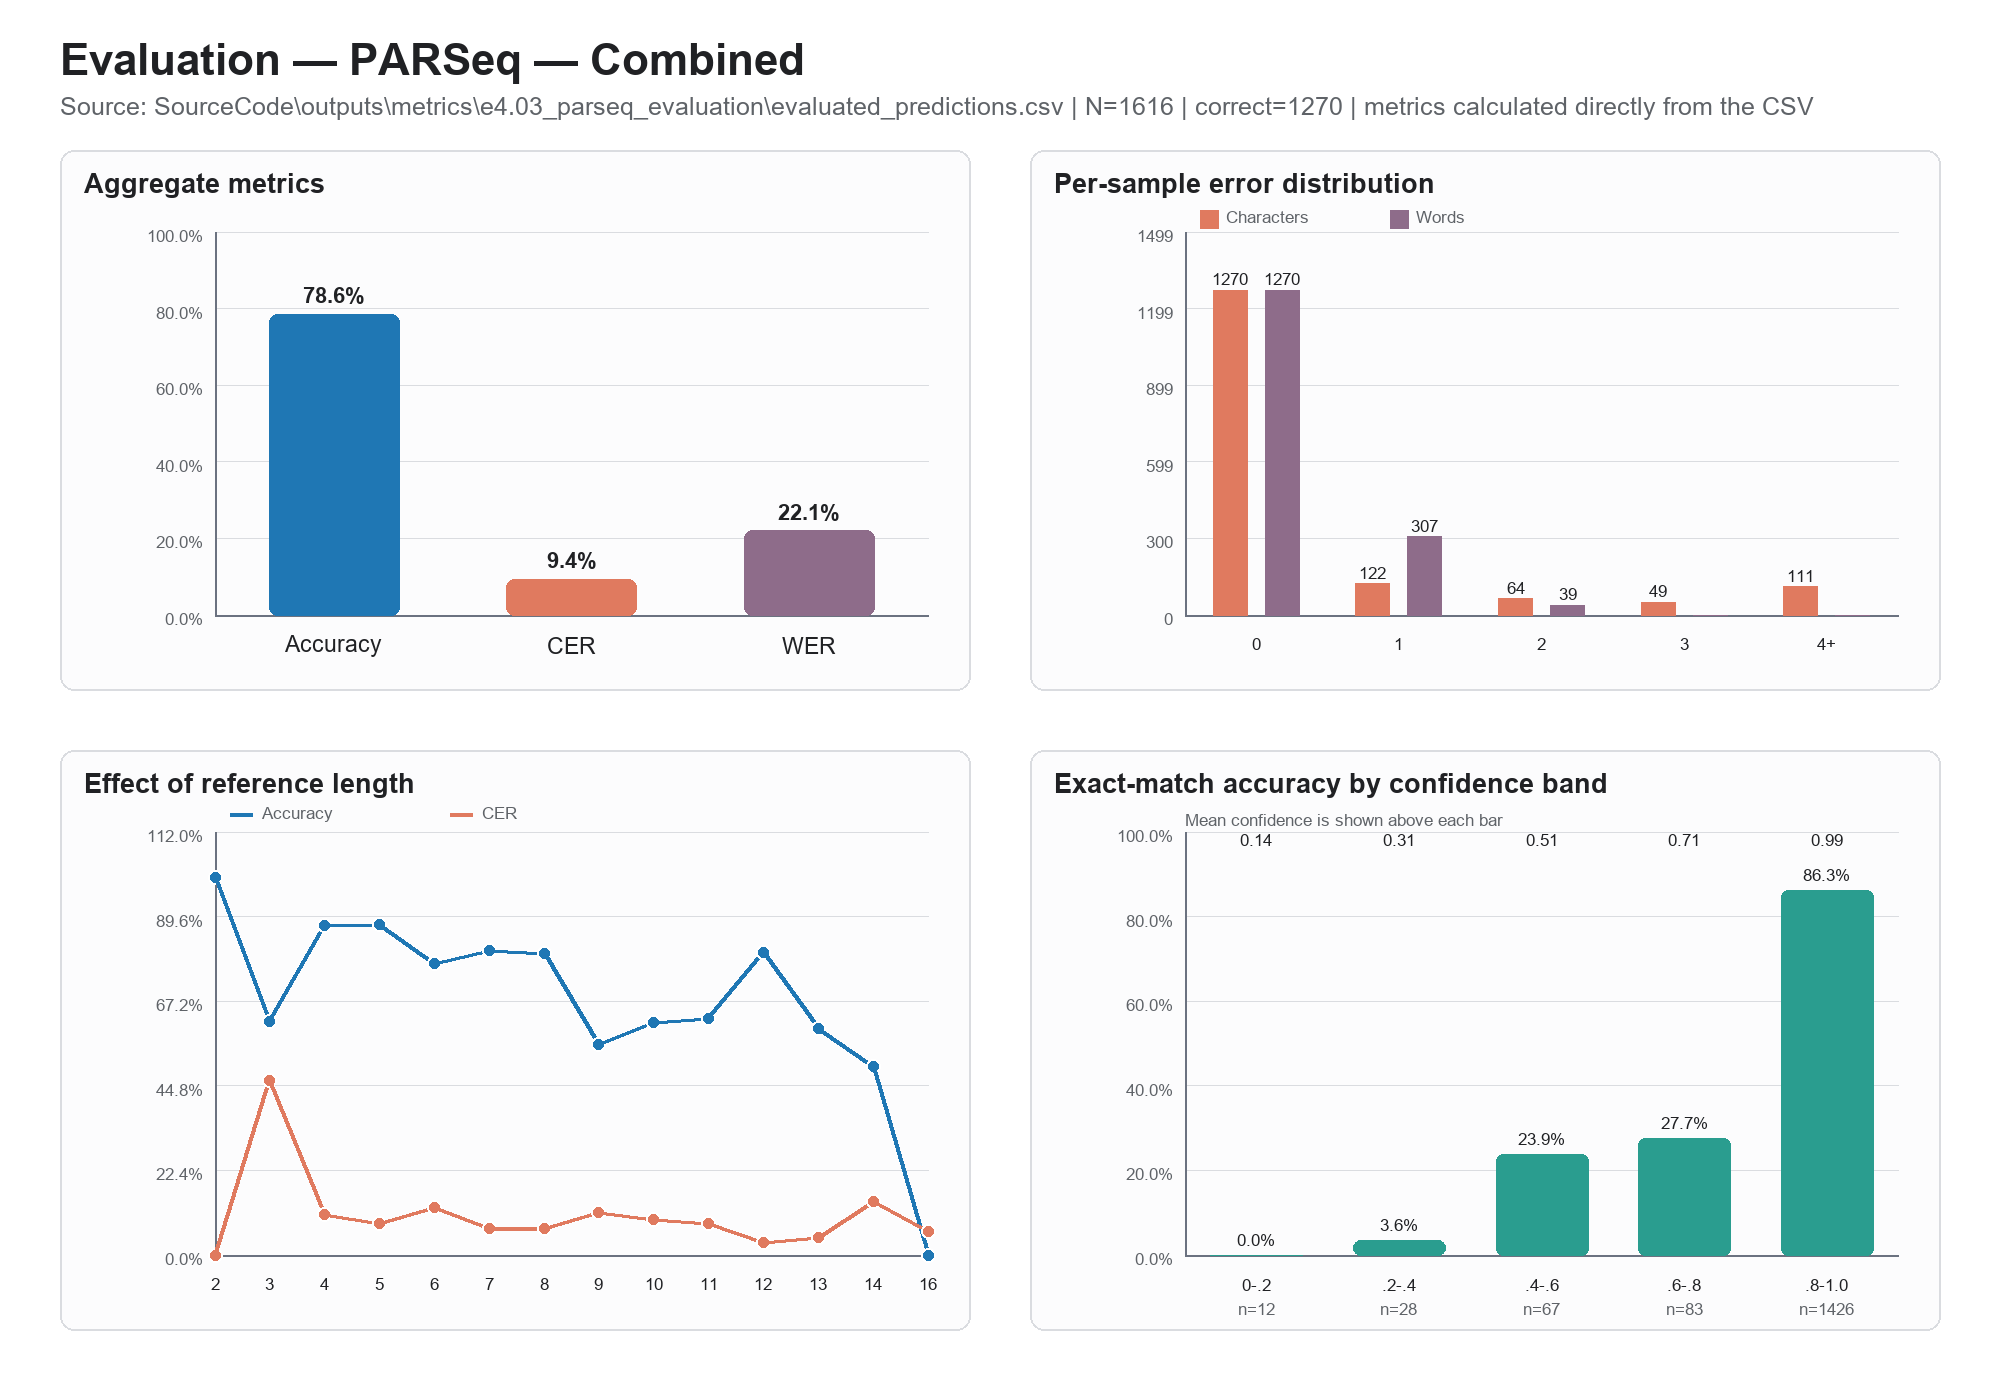
\includegraphics[width=\linewidth]{imagens/evaluation_graficos_tabelas/e4.03_parseq_evaluation_evaluated_predictions.png}
    \caption{Evaluated predictions.}
  \end{subfigure}\hfill
  \begin{subfigure}{0.49\linewidth}
    \centering
    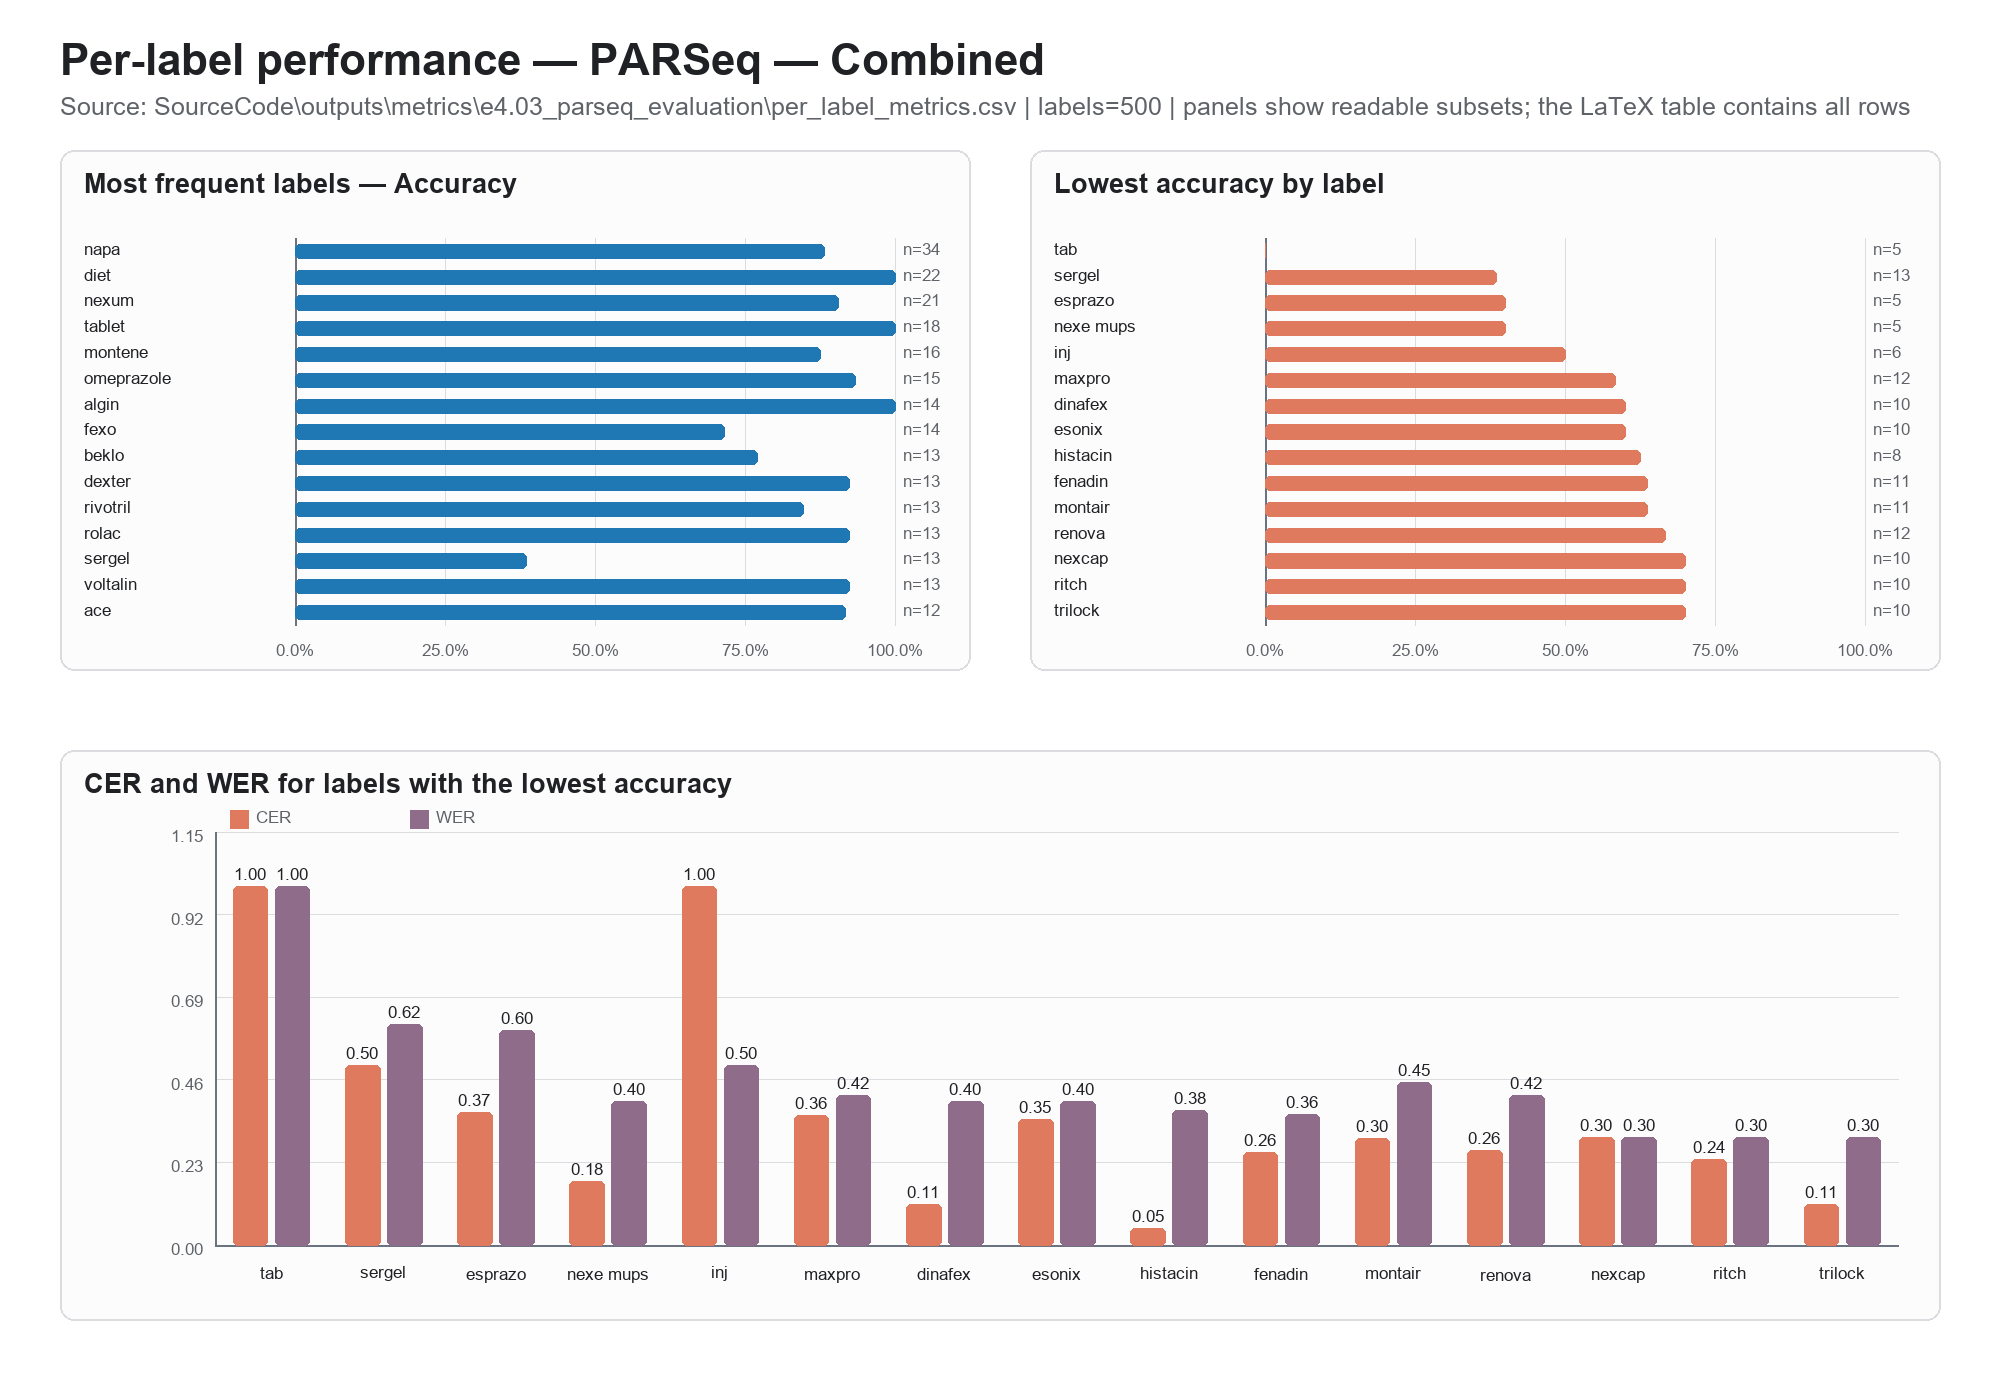
\includegraphics[width=\linewidth]{imagens/evaluation_graficos_tabelas/e4.03_parseq_evaluation_per_label_metrics.png}
    \caption{Per-label metrics.}
  \end{subfigure}
  \caption{PARSeq evaluated in the combined scenario.}
  \label{fig:diagnostic-e4-combined}
\end{figure}

\section{Limitations}
\label{sec:limitations}

This study has limitations related to the amount of available data and the training batch sizes, which were restricted by the available memory capacity. These limitations may have introduced some bias into the results. However, all models were trained and evaluated under the same experimental conditions, using the same computational environment and training configurations, to provide the fairest possible comparison among the methods.


\section{Conclusion}
\label{sec:conclusion}

The results demonstrate the potential of sequence-recognition models for transcribing handwritten words in medical prescriptions. In particular, TrOCR and PARSeq achieved the best performance among the evaluated methods, with consistent advantages over the CNN baseline in all three experimental scenarios. PARSeq performed best on PrescriptionBD, reaching $90.13\%$ accuracy, a CER of $0.0680$, and a WER of $0.1000$, whereas TrOCR achieved the best overall performance in the combined scenario in terms of accuracy ($80.88\%$) and WER ($0.2018$). These results indicate that pre-trained models adapted through \textit{fine-tuning} are an effective strategy for OCR of handwritten medical text, even under limited-data conditions.

\section*{Code and Data Availability}

The code, data, and supplementary materials are available at:
\begin{center}
	\url{https://github.com/SamuelFerrc/Medical-Handwriting-Ocr}
\end{center}

\bibliographystyle{unsrtnat}
\bibliography{references}
\end{document}
